\chapter{Chapter 4. Results}

\renewcommand{\arraystretch}{0.9}

\section{Exploratory Model Runs}

As mentioned in the previous chapter, one of the main challenges encountered while training neural networks is the overwhelming number of independent variables that can affect model performance. These so-called ``hyperparameters'' may have complex interdependence, and there are few general best-practices. In order to identify a reasonable baseline for the performance of each of the model architectures, we started by training a wide variety of permutations on model properties including the number of layers, nodes per layer, activation function, and prediction coarseness, as well as training properties including loss function characteristics, batch normalization, and weight dropout rate. At this stage, developing a rigorous understanding of the effects of changes in model and training setup was not a priority; instead, we modified multiple hyperparameters simultaneously between training iterations with the goal of establishing rough rules of thumb and a sense for the approximate size of models needed for this task.

\begin{figure}[hp!]
    \centering
    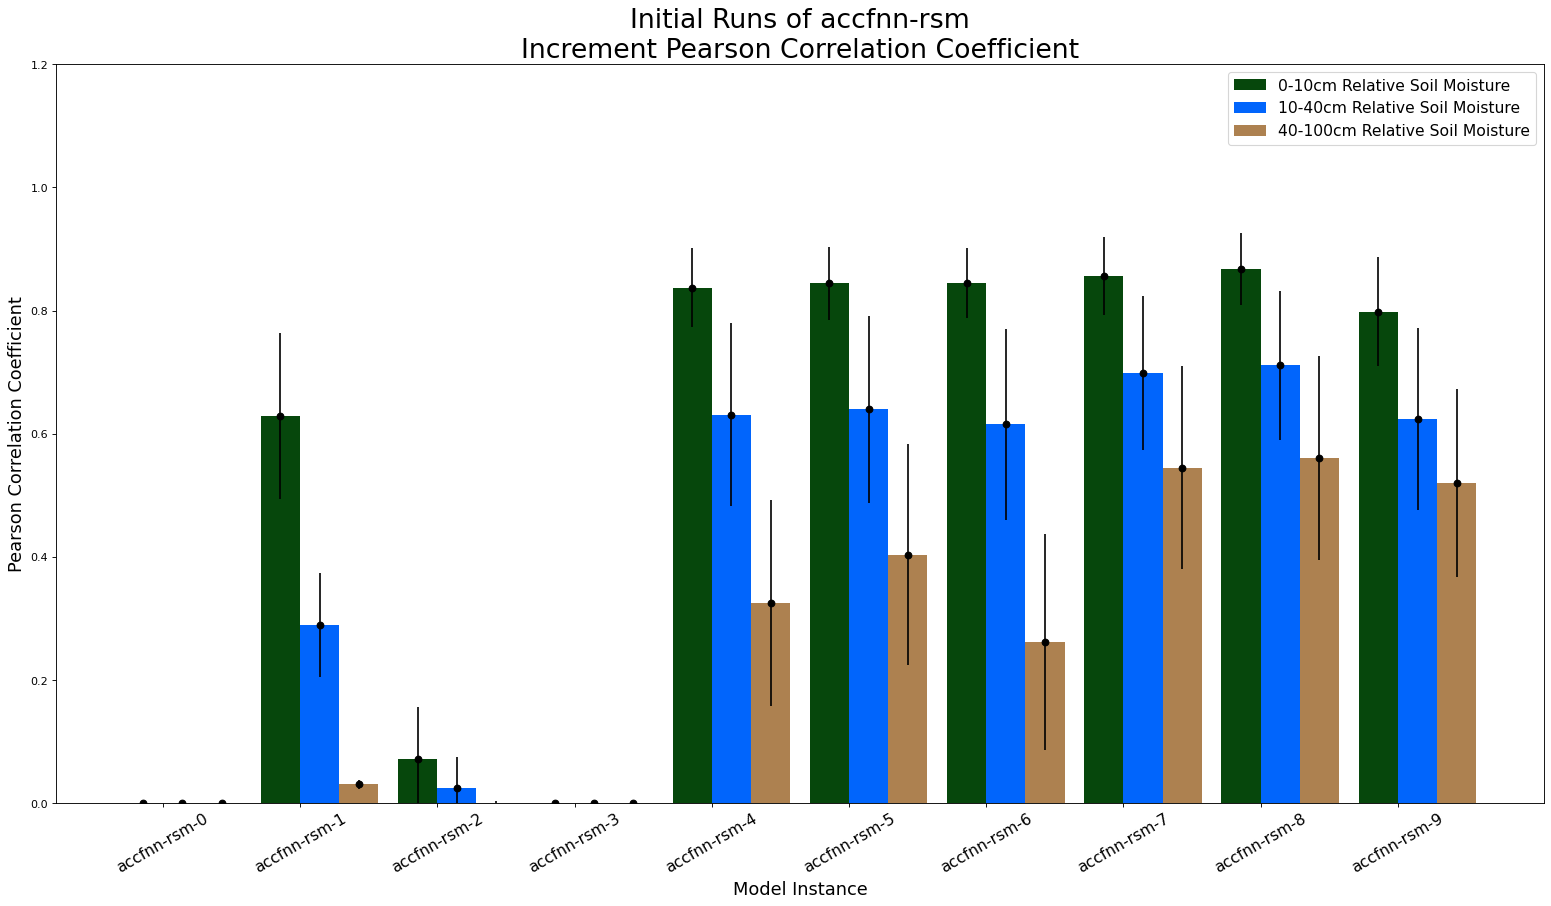
\includegraphics[width=.48\linewidth,draft=false]{figures/efficiency_initial-best/eval_test_efficiency_initial-accfnn-rsm_cc_res.png}
    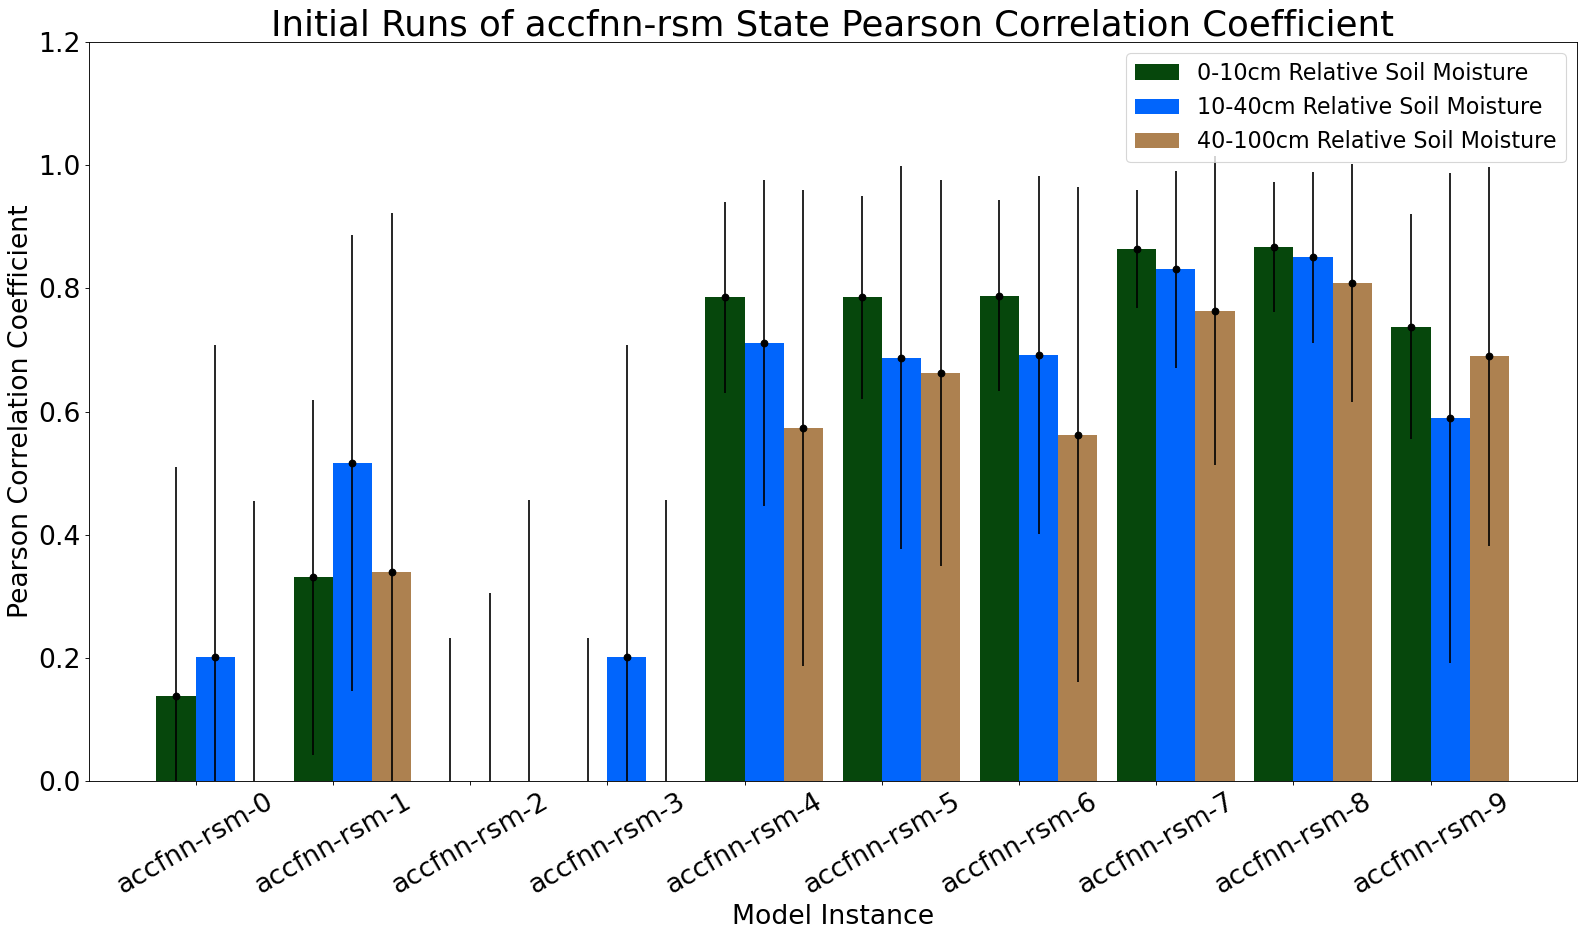
\includegraphics[width=.48\linewidth,draft=false]{figures/efficiency_initial-best/eval_test_efficiency_initial-accfnn-rsm_cc_state.png}

    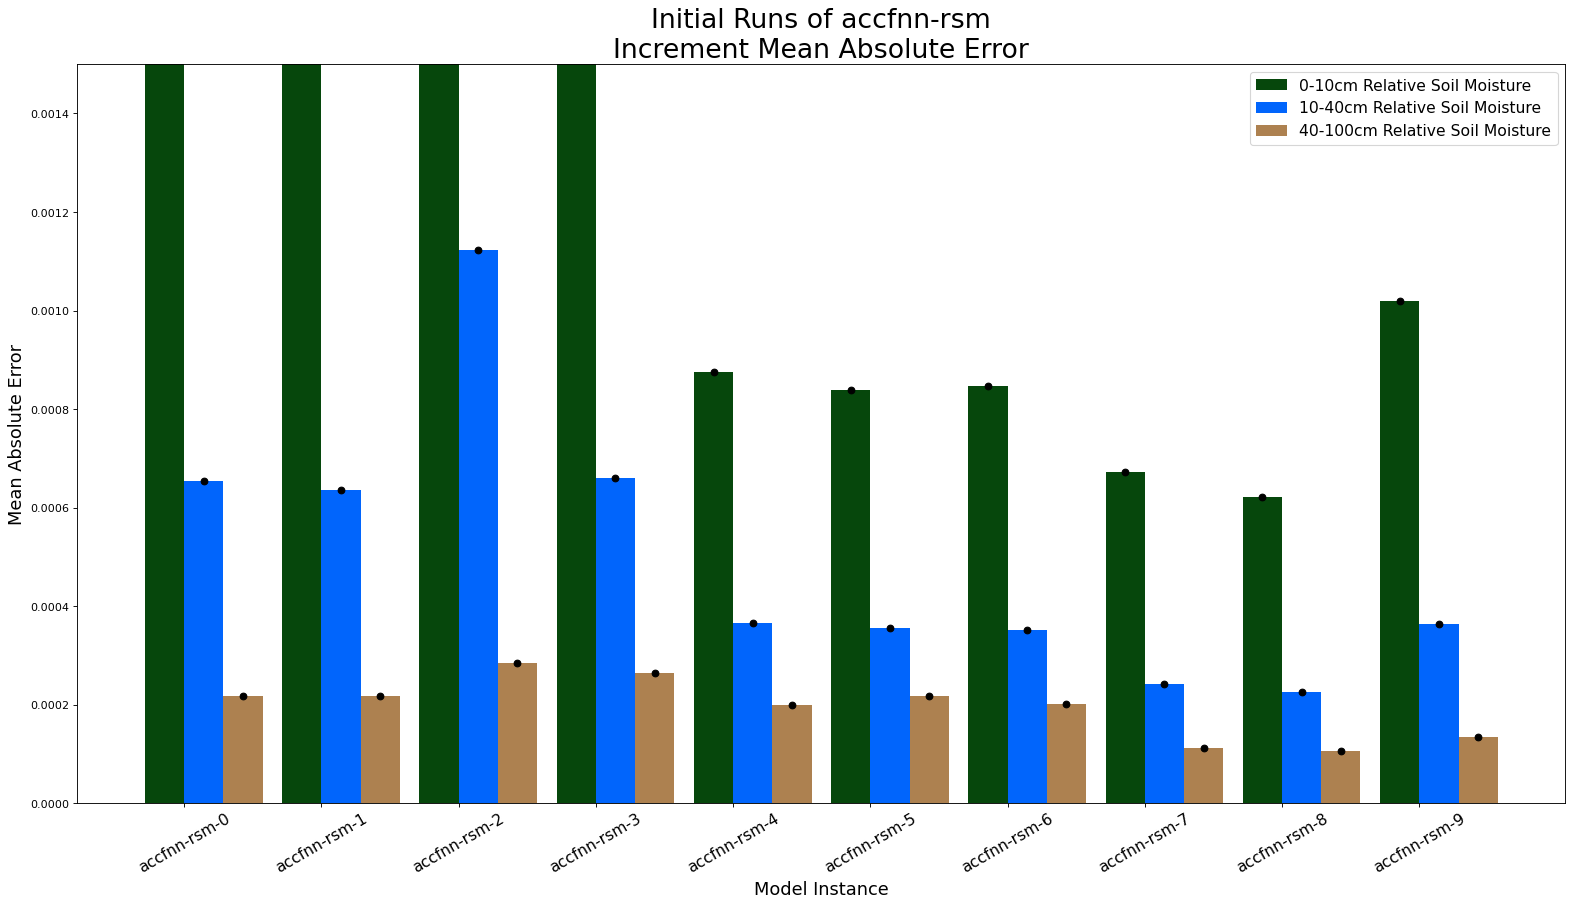
\includegraphics[width=.48\linewidth,draft=false]{figures/efficiency_initial-best/eval_test_efficiency_initial-accfnn-rsm_mae_res.png}
    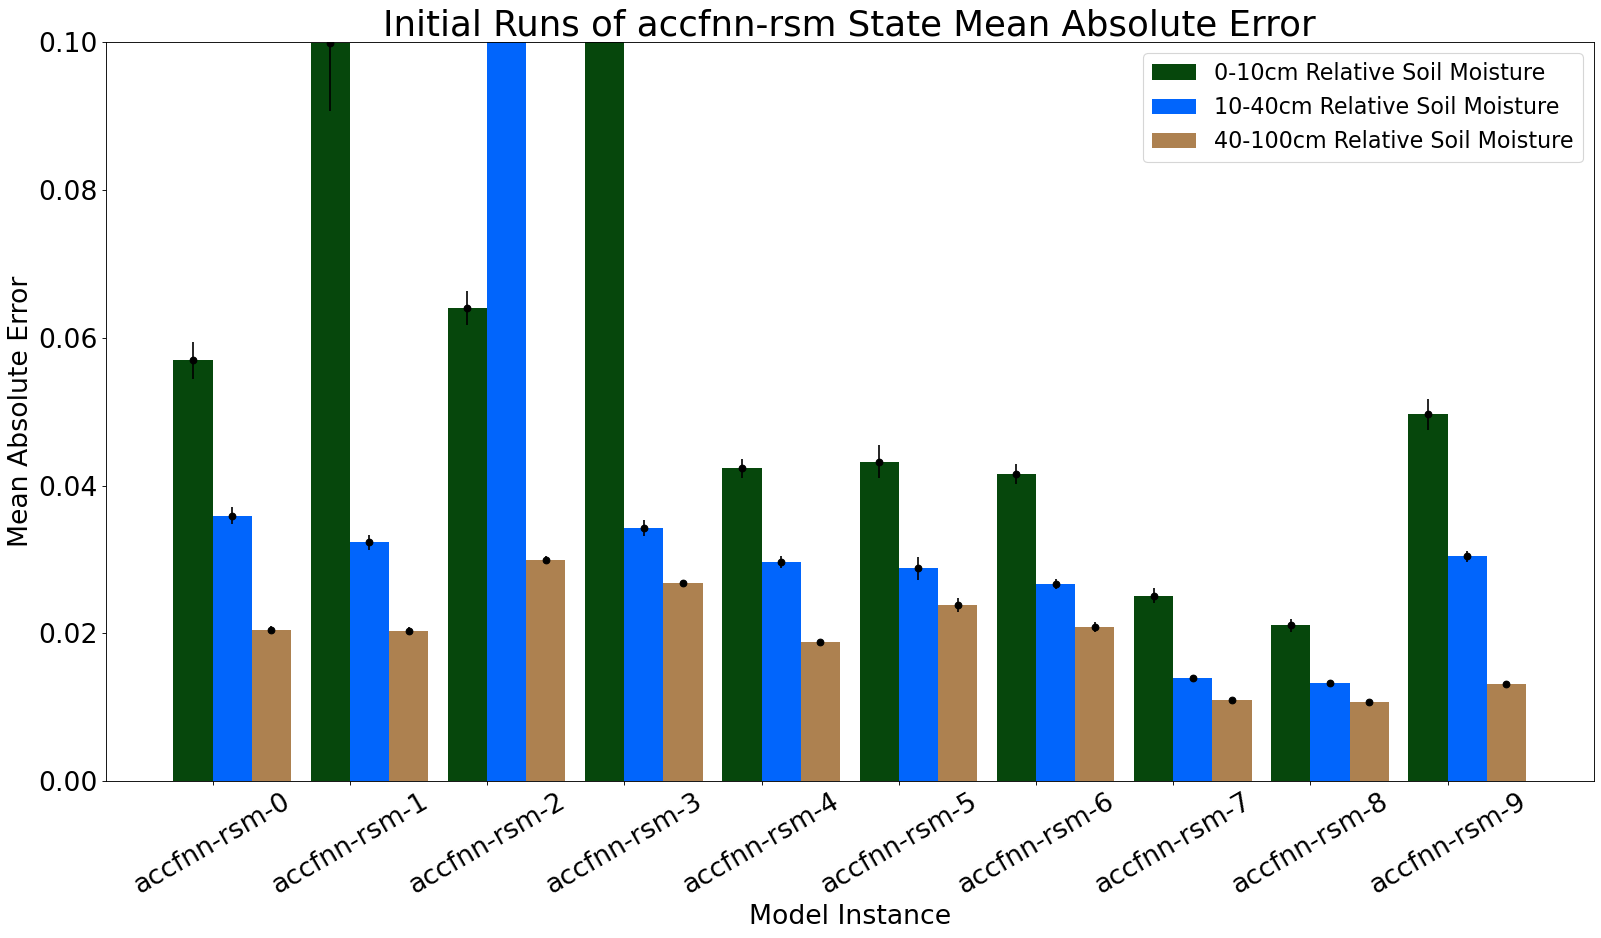
\includegraphics[width=.48\linewidth,draft=false]{figures/efficiency_initial-best/eval_test_efficiency_initial-accfnn-rsm_mae_state.png}

    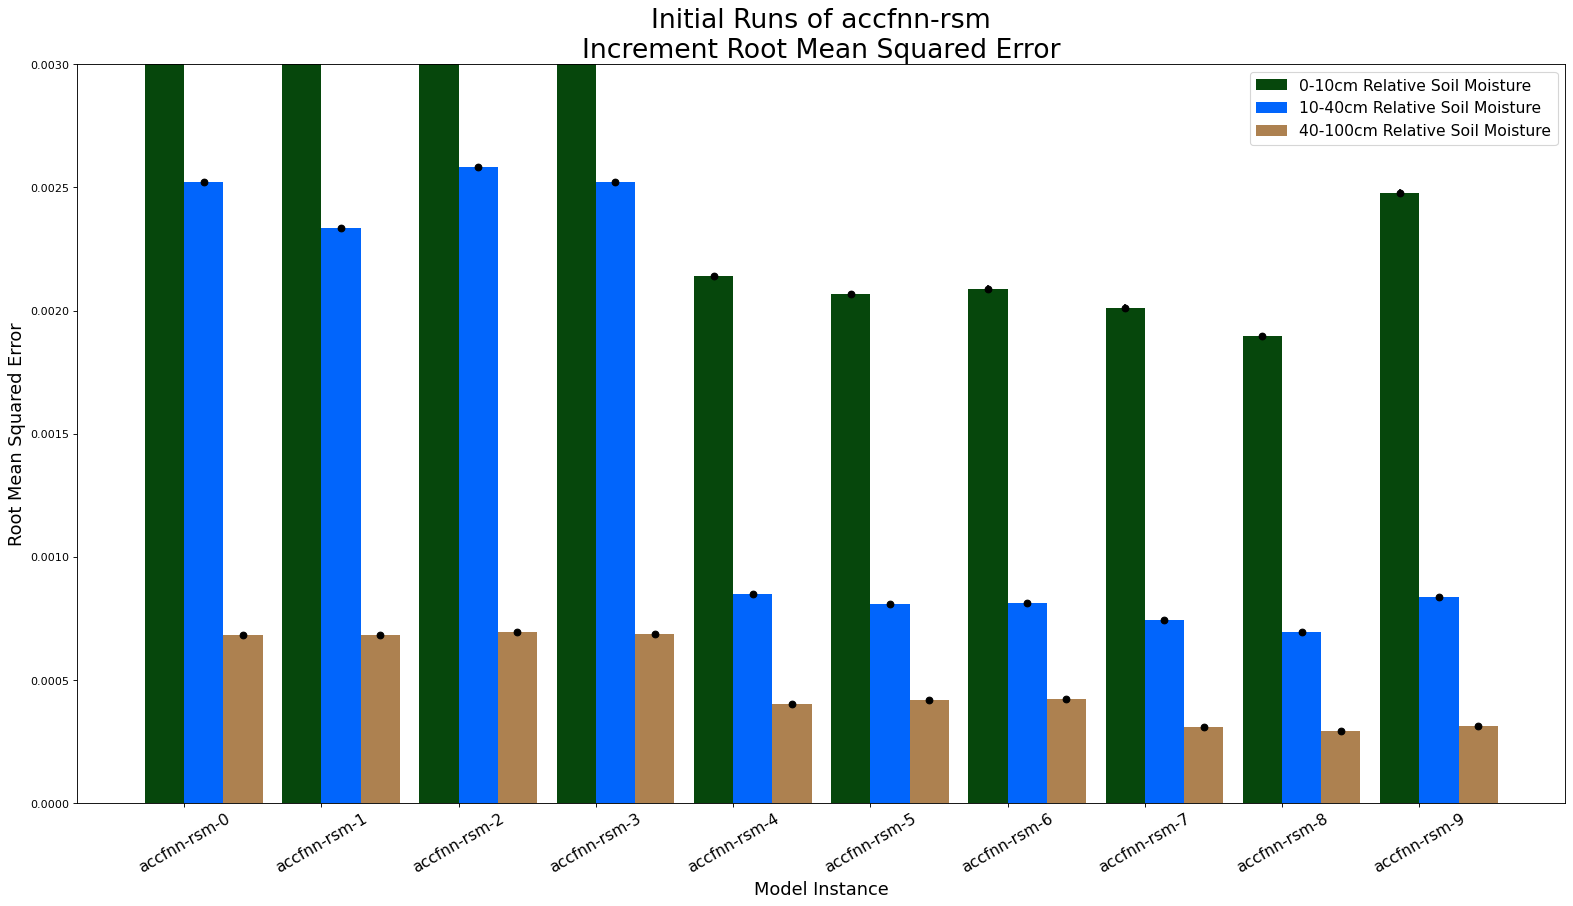
\includegraphics[width=.48\linewidth,draft=false]{figures/efficiency_initial-best/eval_test_efficiency_initial-accfnn-rsm_mse_res.png}
    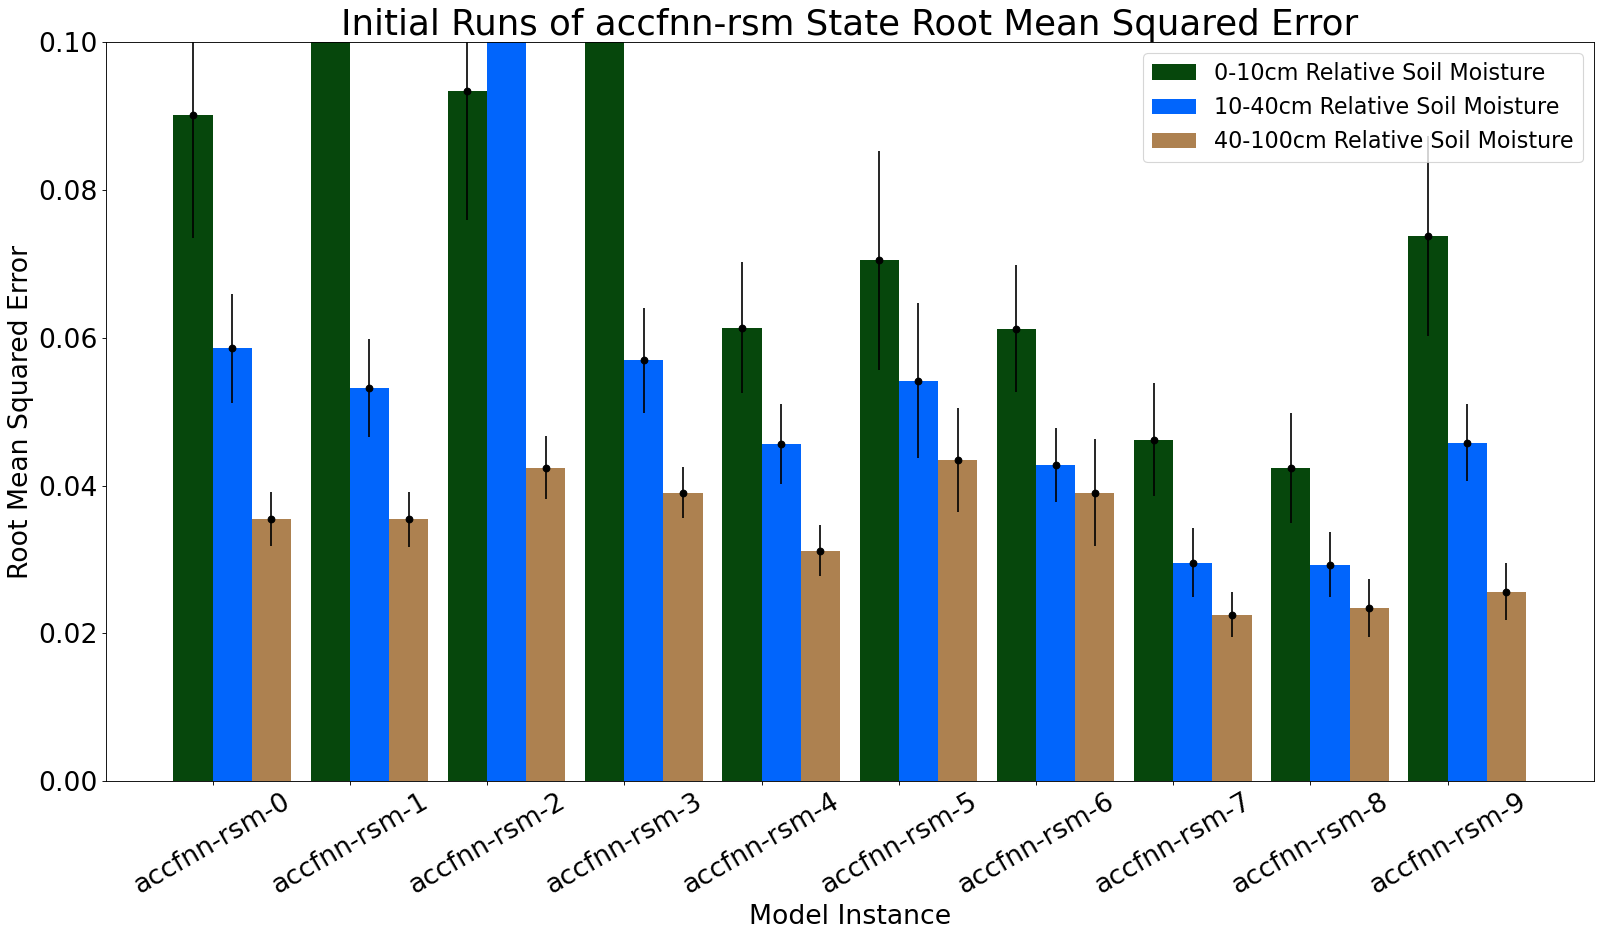
\includegraphics[width=.48\linewidth,draft=false]{figures/efficiency_initial-best/eval_test_efficiency_initial-accfnn-rsm_mse_state.png}

    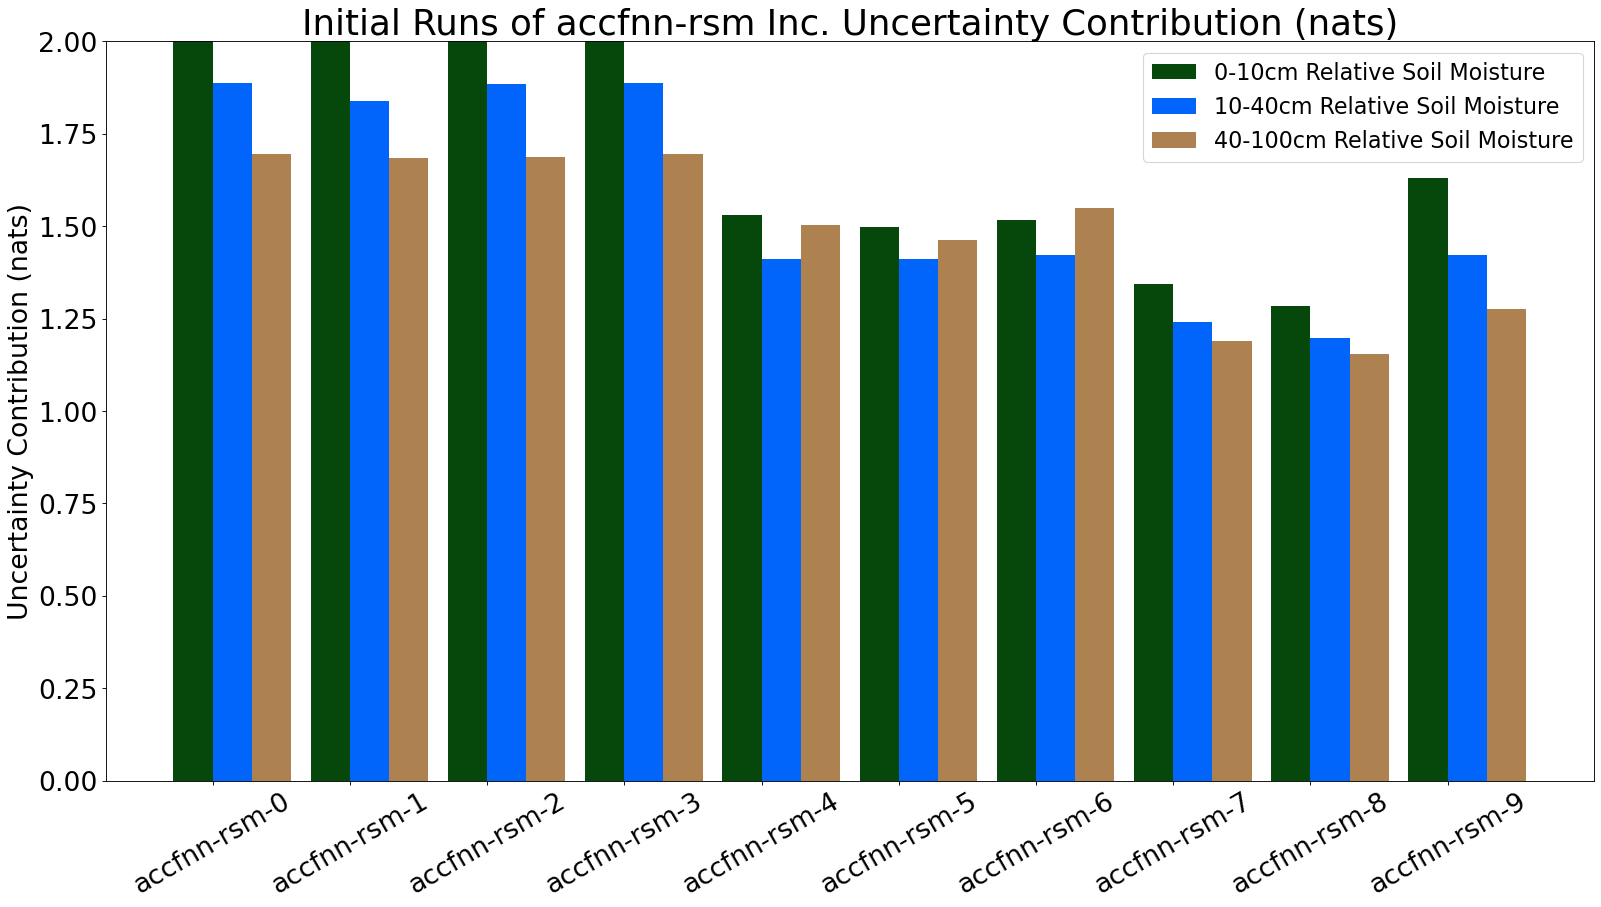
\includegraphics[width=.48\linewidth,draft=false]{figures/efficiency_initial-best/eval_test_efficiency_initial-accfnn-rsm_info-loss_res.png}
    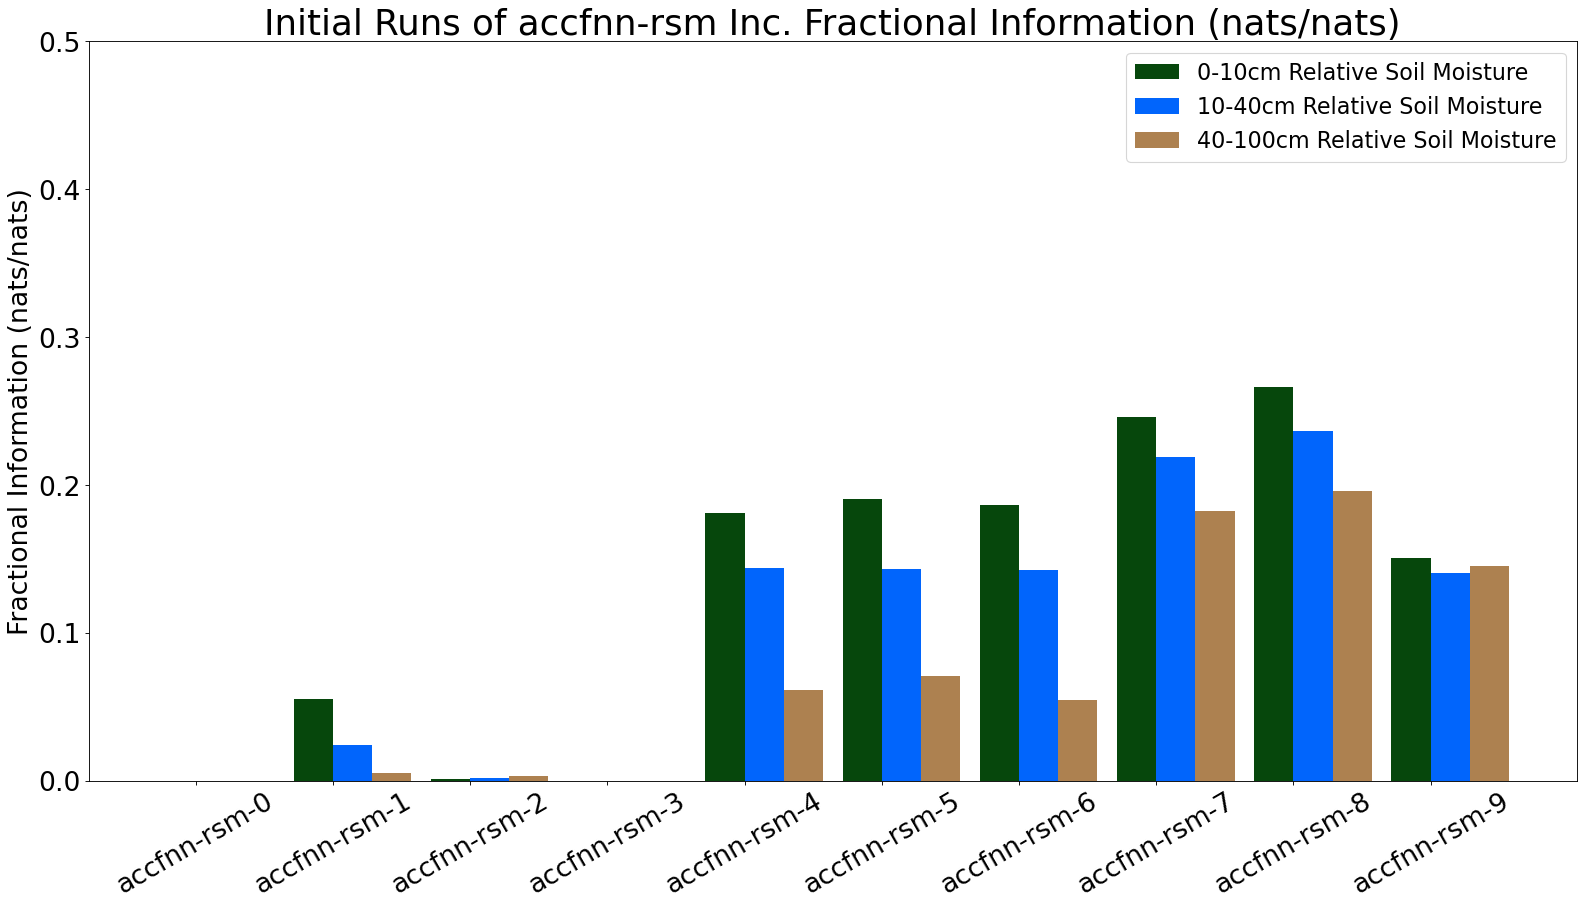
\includegraphics[width=.48\linewidth,draft=false]{figures/efficiency_initial-best/eval_test_efficiency_initial-accfnn-rsm_fi_res.png}

    \caption{Bulk metrics for initial FNN training runs}
    \label{model-init-fnn}
\end{figure}

\begin{table}[h!p]
    \footnotesize
    \centering
\begin{sideways}
    \begin{tabular}{c|c|c|c|c|c|c }
Name & Desc & Weights & \thead{State\\MAE} & \thead{State\\CC} & \thead{Info\\Loss} &\thead{Frac.\\Info}\\
\hline
\multirow{3}{6em}{accfnn-rsm-0} & \multirow{3}{16em}{First FNN} & \multirow{3}{4em}{14203} & 0.057 & 0.139 & 2.196 & 0.000 \\ & & & 0.036 & 0.201 & 1.889 & 0.000 \\ & & & 0.020 & -0.215 & 1.694 & 0.000 \\
\hline
\multirow{3}{6em}{accfnn-rsm-1} & \multirow{3}{16em}{Same setup as accrnn-rsm-1 but only a FNN} & \multirow{3}{4em}{14203} & 0.100 & 0.331 & 2.065 & 0.055 \\ & & & 0.032 & 0.517 & 1.840 & 0.024 \\ & & & 0.020 & 0.340 & 1.685 & 0.005 \\
\hline
\multirow{3}{6em}{accfnn-rsm-2} & \multirow{3}{16em}{Much wider and deeper, MSE loss, more dropout} & \multirow{3}{4em}{85947} & 0.064 & -0.139 & 2.193 & 0.001 \\ & & & 0.102 & -0.201 & 1.885 & 0.002 \\ & & & 0.030 & -0.214 & 1.688 & 0.003 \\
\hline
\multirow{3}{6em}{accfnn-rsm-3} & \multirow{3}{16em}{Same as fnn-2 but ignoring constant targets} & \multirow{3}{4em}{85947} & 0.113 & -0.139 & 2.196 & 0.000 \\ & & & 0.034 & 0.201 & 1.889 & 0.000 \\ & & & 0.027 & -0.215 & 1.694 & 0.000 \\
\hline
\multirow{3}{6em}{accfnn-rsm-4} & \multirow{3}{16em}{Same as rsm-2 but no dropout, higher increment magnitude bias} & \multirow{3}{4em}{85947} & 0.042 & 0.786 & 1.530 & 0.181 \\ & & & 0.030 & 0.711 & 1.412 & 0.144 \\ & & & 0.019 & 0.573 & 1.502 & 0.061 \\
\hline
\multirow{3}{6em}{accfnn-rsm-5} & \multirow{3}{16em}{Same as rsm-4 but ignoring constant targets} & \multirow{3}{4em}{85947} & 0.043 & 0.785 & 1.499 & 0.191 \\ & & & 0.029 & 0.688 & 1.411 & 0.143 \\ & & & 0.024 & 0.663 & 1.463 & 0.071 \\
\hline
\multirow{3}{6em}{accfnn-rsm-6} & \multirow{3}{16em}{Same as rsm-4 but narrower and deeper} & \multirow{3}{4em}{30843} & 0.042 & 0.788 & 1.516 & 0.187 \\ & & & 0.027 & 0.692 & 1.423 & 0.142 \\ & & & 0.021 & 0.563 & 1.550 & 0.055 \\
\hline
\multirow{3}{6em}{accfnn-rsm-7} & \multirow{3}{16em}{Same as rsm-6 but mae loss} & \multirow{3}{4em}{30843} & 0.025 & 0.864 & 1.343 & 0.246 \\ & & & 0.014 & 0.831 & 1.242 & 0.219 \\ & & & 0.011 & 0.764 & 1.189 & 0.183 \\
\hline
\multirow{3}{6em}{accfnn-rsm-8} & \multirow{3}{16em}{Same as rsm-7 but ignoring constant targets} & \multirow{3}{4em}{30843} & 0.021 & 0.867 & 1.283 & 0.266 \\ & & & 0.013 & 0.850 & 1.197 & 0.236 \\ & & & 0.011 & 0.809 & 1.154 & 0.196 \\
\hline
\multirow{3}{6em}{accfnn-rsm-9} & \multirow{3}{16em}{fnn 5 but actually using increment norm coefficients} & \multirow{3}{4em}{85947} & 0.050 & 0.738 & 1.632 & 0.151 \\ & & & 0.030 & 0.589 & 1.423 & 0.140 \\ & & & 0.013 & 0.689 & 1.277 & 0.145 \\
    \end{tabular}
\end{sideways}
    \caption{Initial fully-connected neural network properties and bulk statistics.}
    \label{model-init-fnn-table}
\end{table}

All of the bulk statistics in this section are reported in terms of relative soil moisture. The bar charts of correlation coefficient, mean absolute error, and mean squared error separately display the error in hourly increment change and integrated soil state, while the entropy-based metrics (uncertainty contribution and fractional information) are calculated only for the increment change. Tables include metrics for each of the depth levels from top to bottom: 0-10cm, 10-40cm, and 40-100cm.

The validation loss of each of the ANN variants generally stopped decreasing after about 18 hours of training on a CPU, though the training time of individual models unsurprisingly depended most strongly on the size of the model and the learning rate parameters. The models shown here have a number of trainable parameters on the order of 100,000. The best-performing instances of the simplest architecture variant (accfnn-rsm-8) had only about 31,000 parameters and used mean absolute error as the base loss function. The FNN instances struggled to converge any time dropout was used during training, and the predictive skill of best model seemed to improve in the lower two layers in response to a loss function manipulation that ignored prediction cost associated with timesteps where the true magnitude of change in soil moisture state was close to zero. Furthermore, the best FNN did not consider error in state within the loss function (increment loss ratio $\rho = 1$), but was trained with a considerable increment magnitude bias of $\gamma = 60$. The network consisted of 8 fully-connected layers each with 64 nodes.

\begin{figure}[hp!]
    \centering
    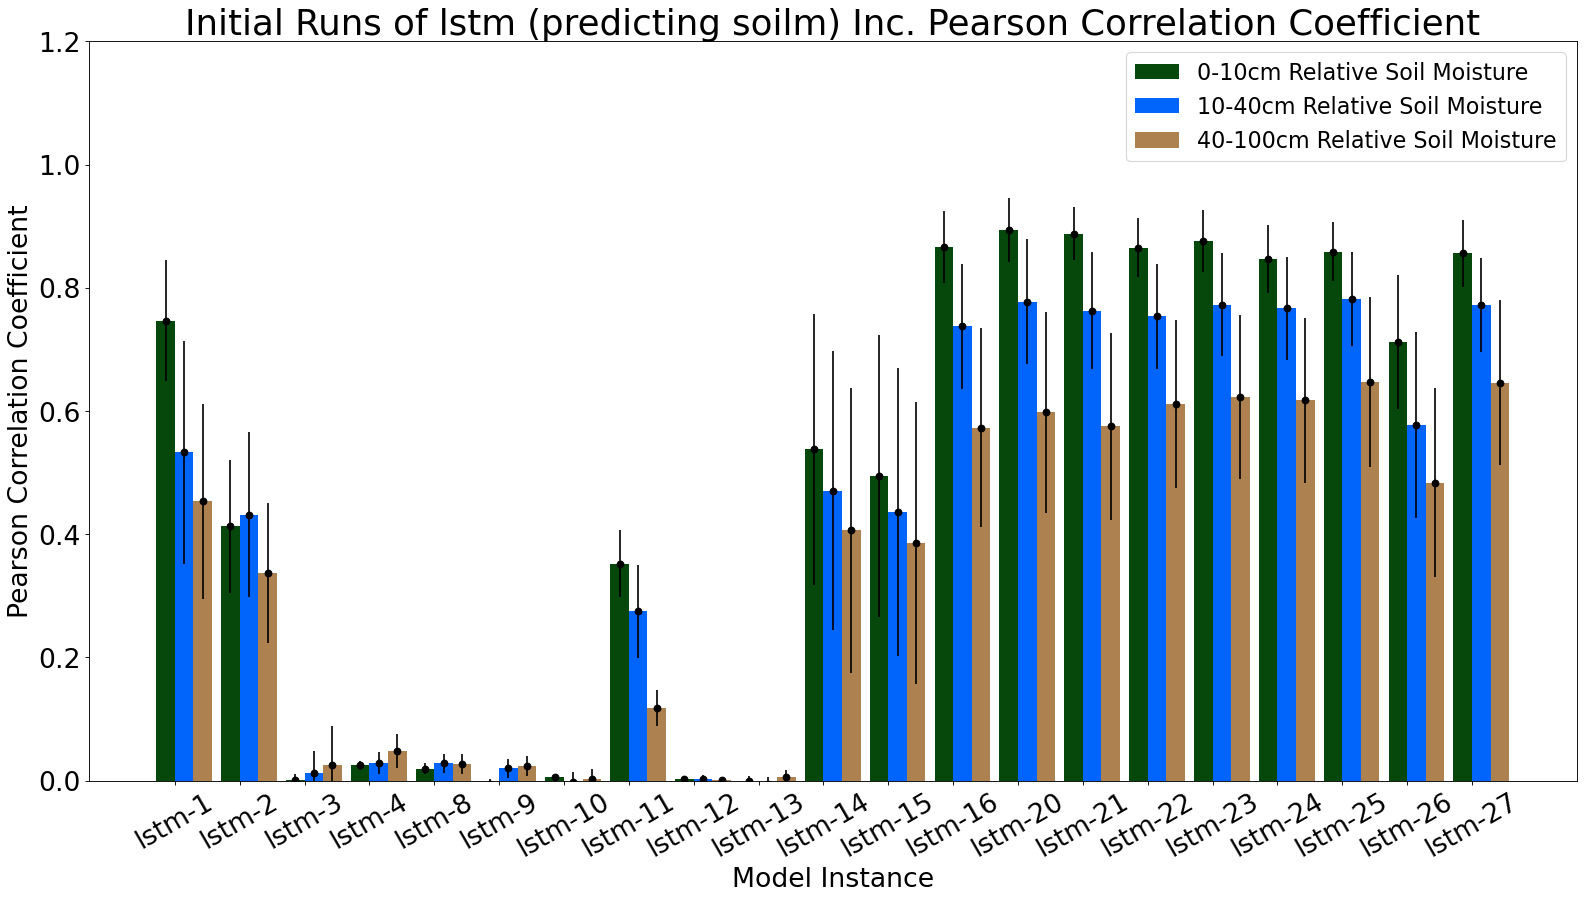
\includegraphics[width=.48\linewidth,draft=false]{figures/efficiency_initial-best/eval_test_efficiency_initial-lstm-soilm_cc_res.png}
    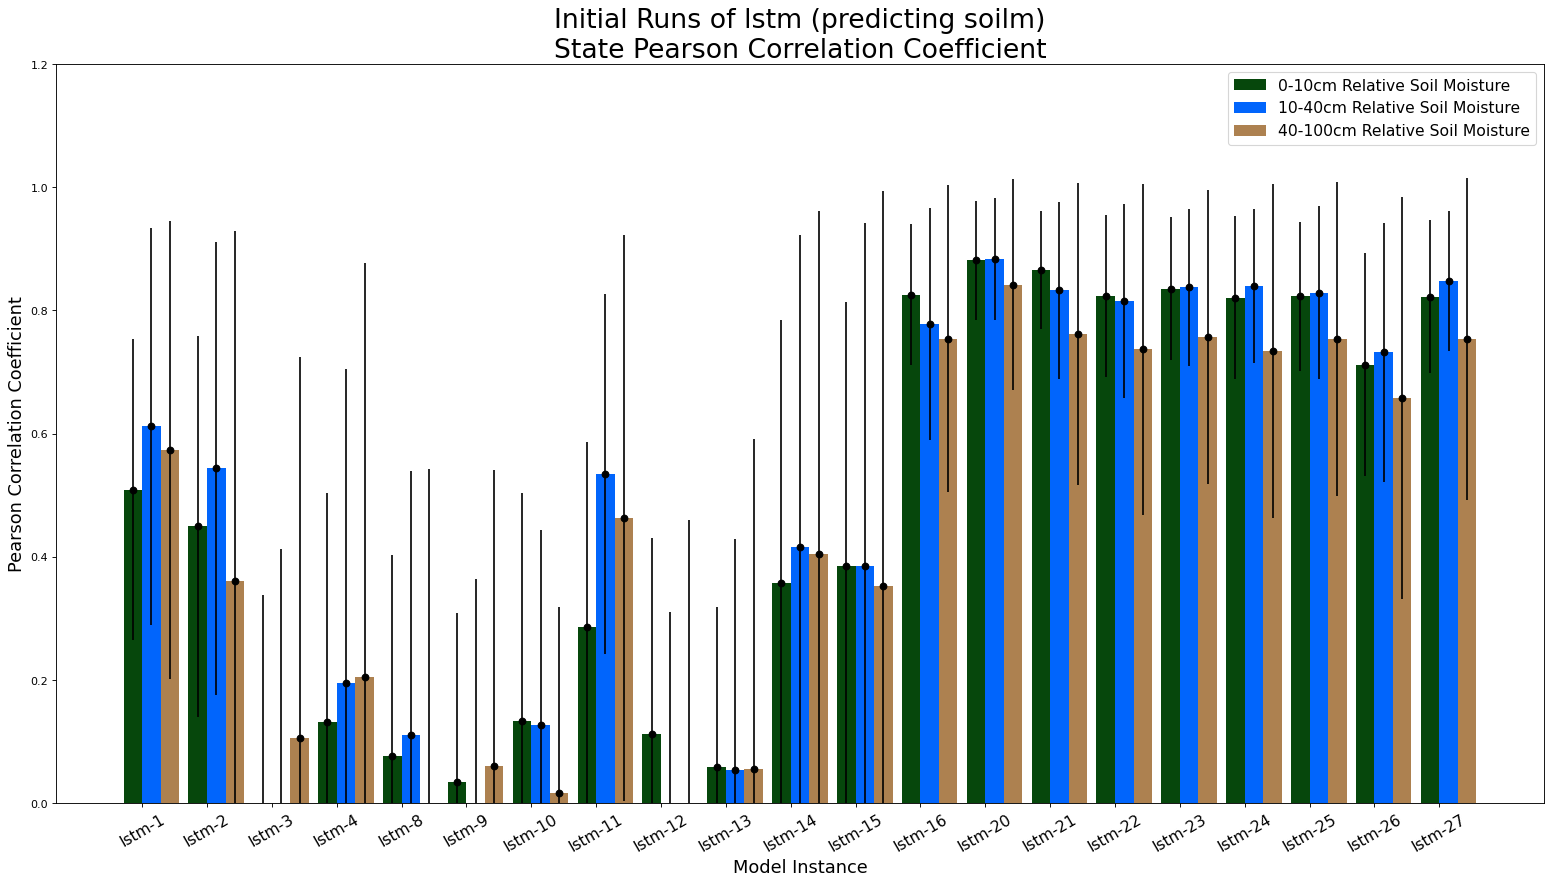
\includegraphics[width=.48\linewidth,draft=false]{figures/efficiency_initial-best/eval_test_efficiency_initial-lstm-soilm_cc_state.png}

    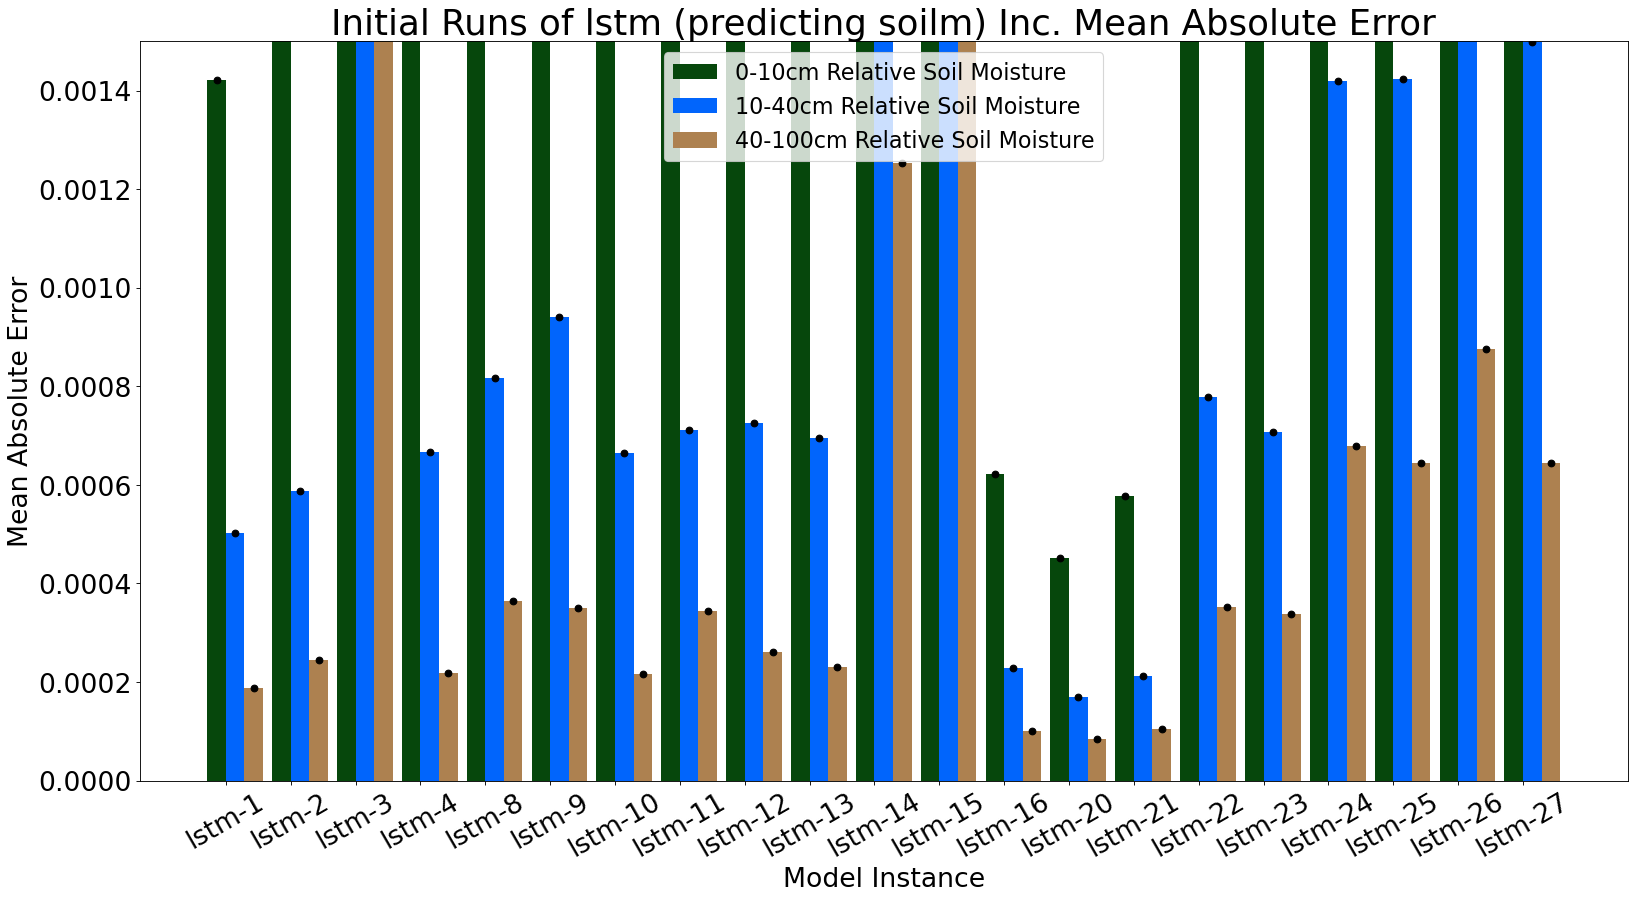
\includegraphics[width=.48\linewidth,draft=false]{figures/efficiency_initial-best/eval_test_efficiency_initial-lstm-soilm_mae_res.png}
    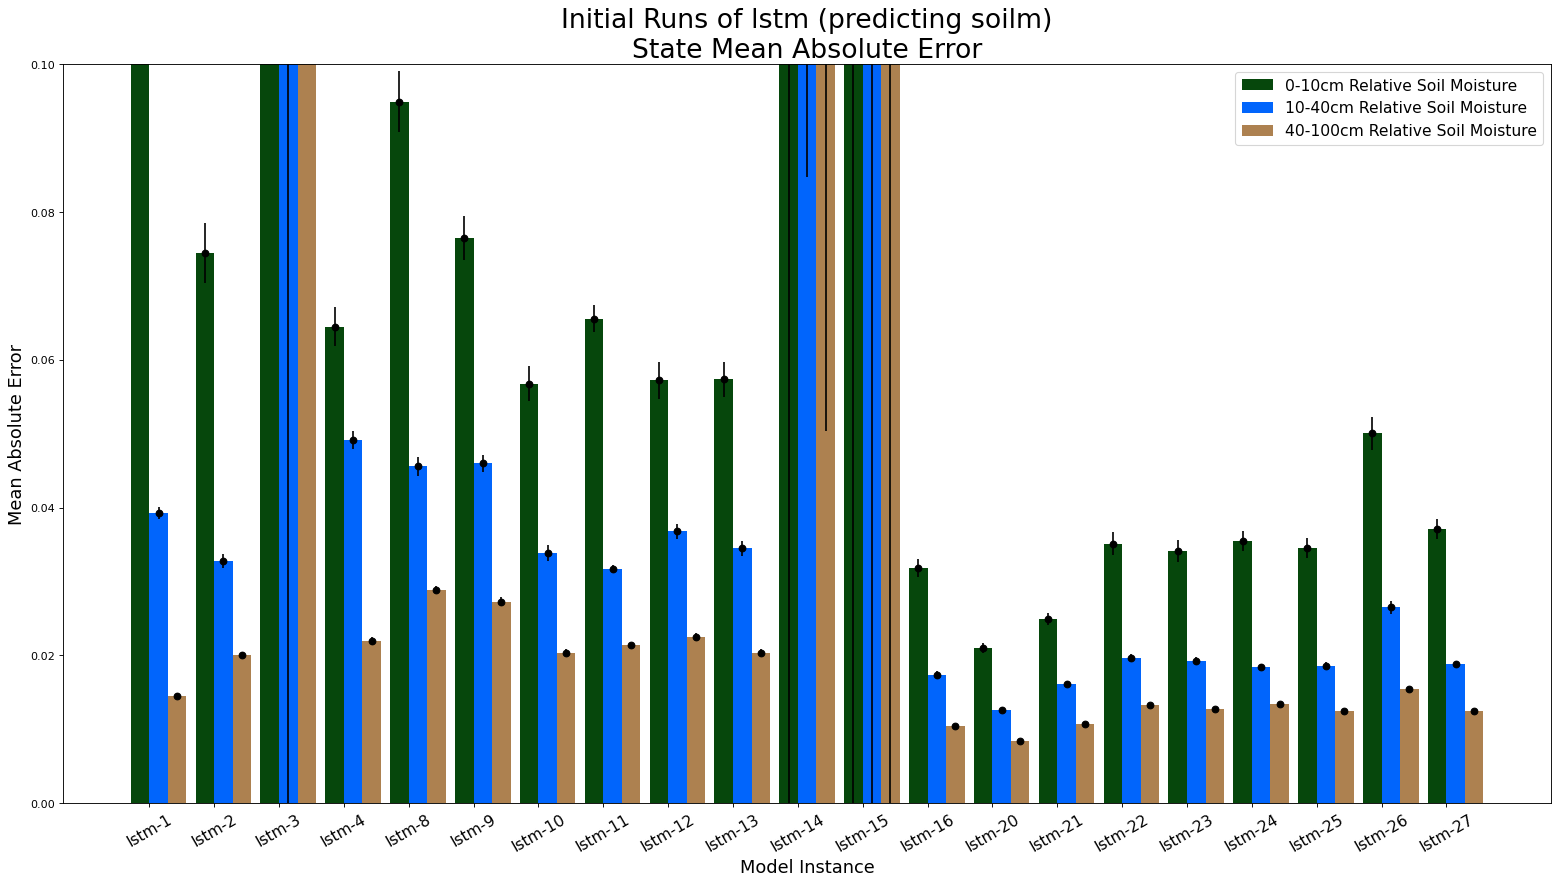
\includegraphics[width=.48\linewidth,draft=false]{figures/efficiency_initial-best/eval_test_efficiency_initial-lstm-soilm_mae_state.png}

    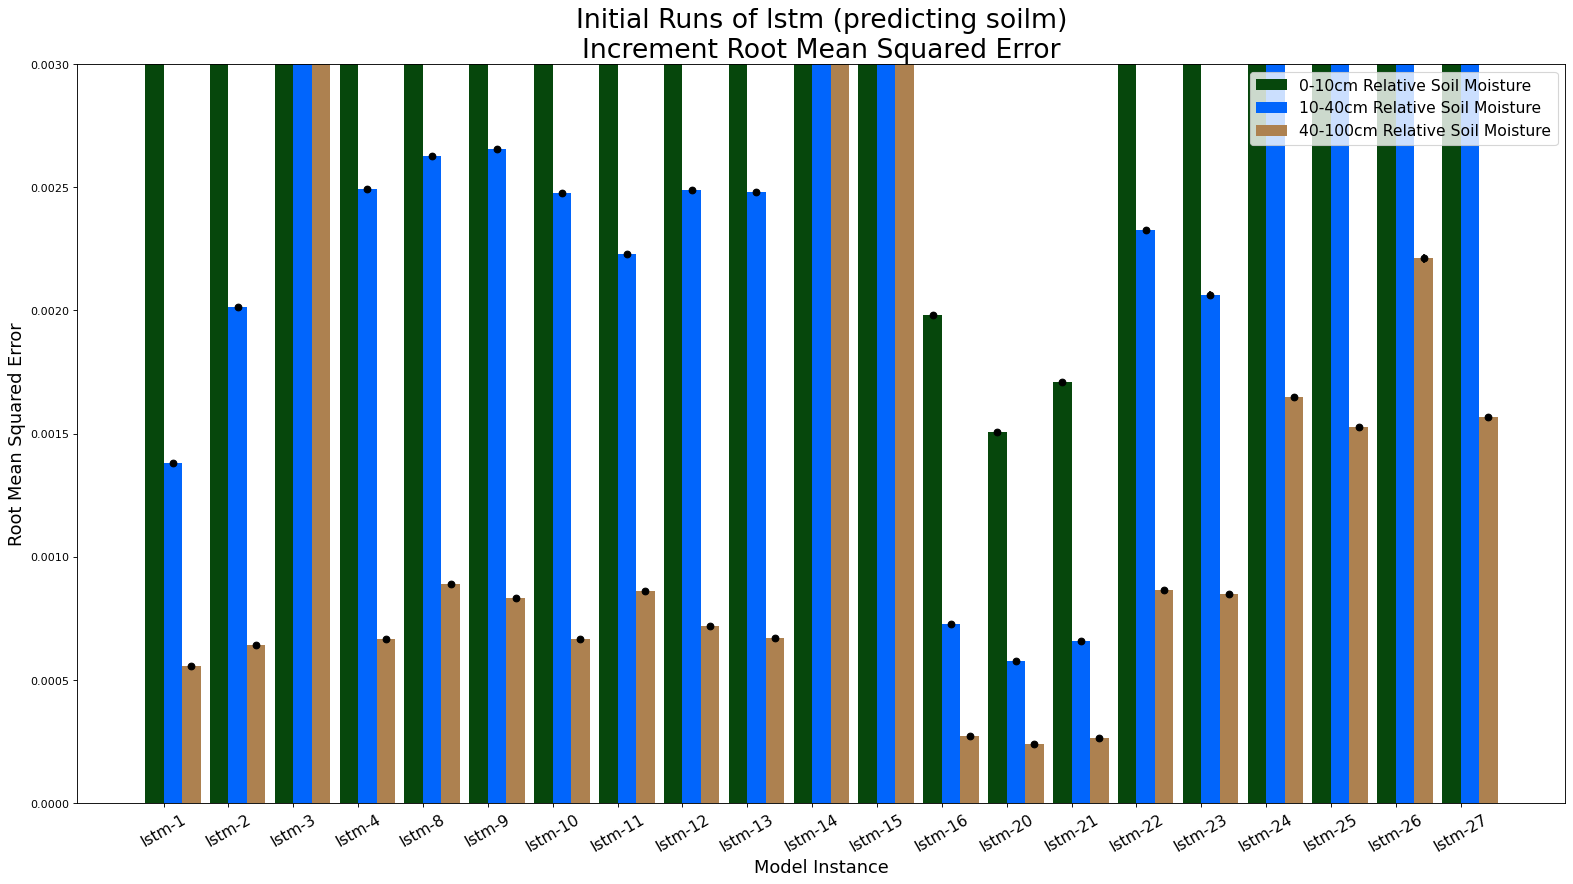
\includegraphics[width=.48\linewidth,draft=false]{figures/efficiency_initial-best/eval_test_efficiency_initial-lstm-soilm_mse_res.png}
    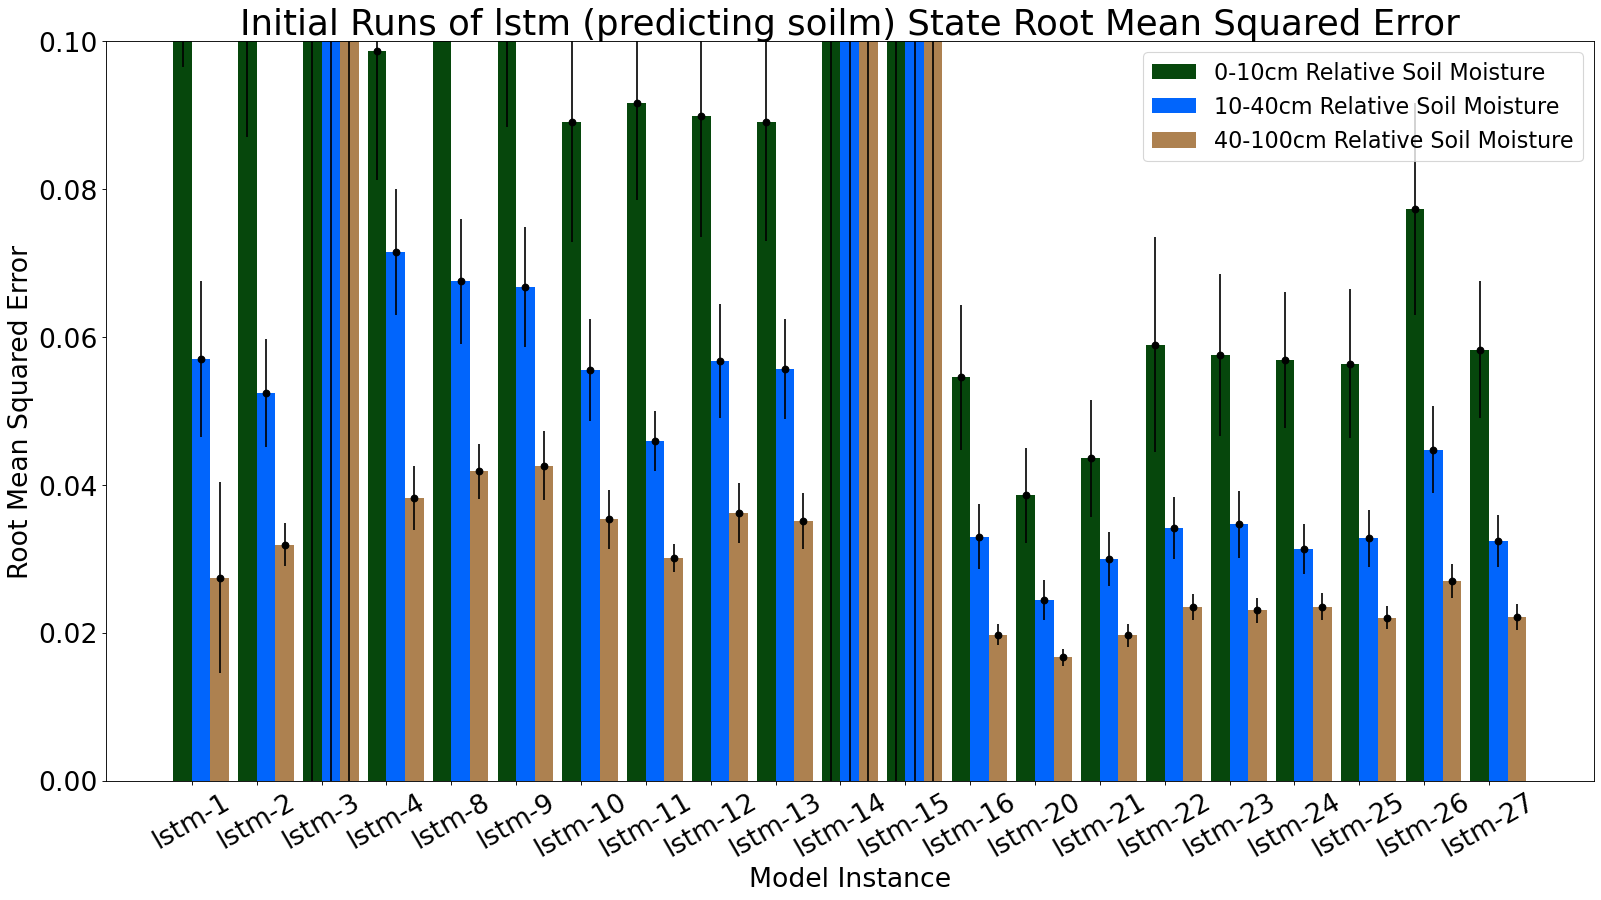
\includegraphics[width=.48\linewidth,draft=false]{figures/efficiency_initial-best/eval_test_efficiency_initial-lstm-soilm_mse_state.png}

    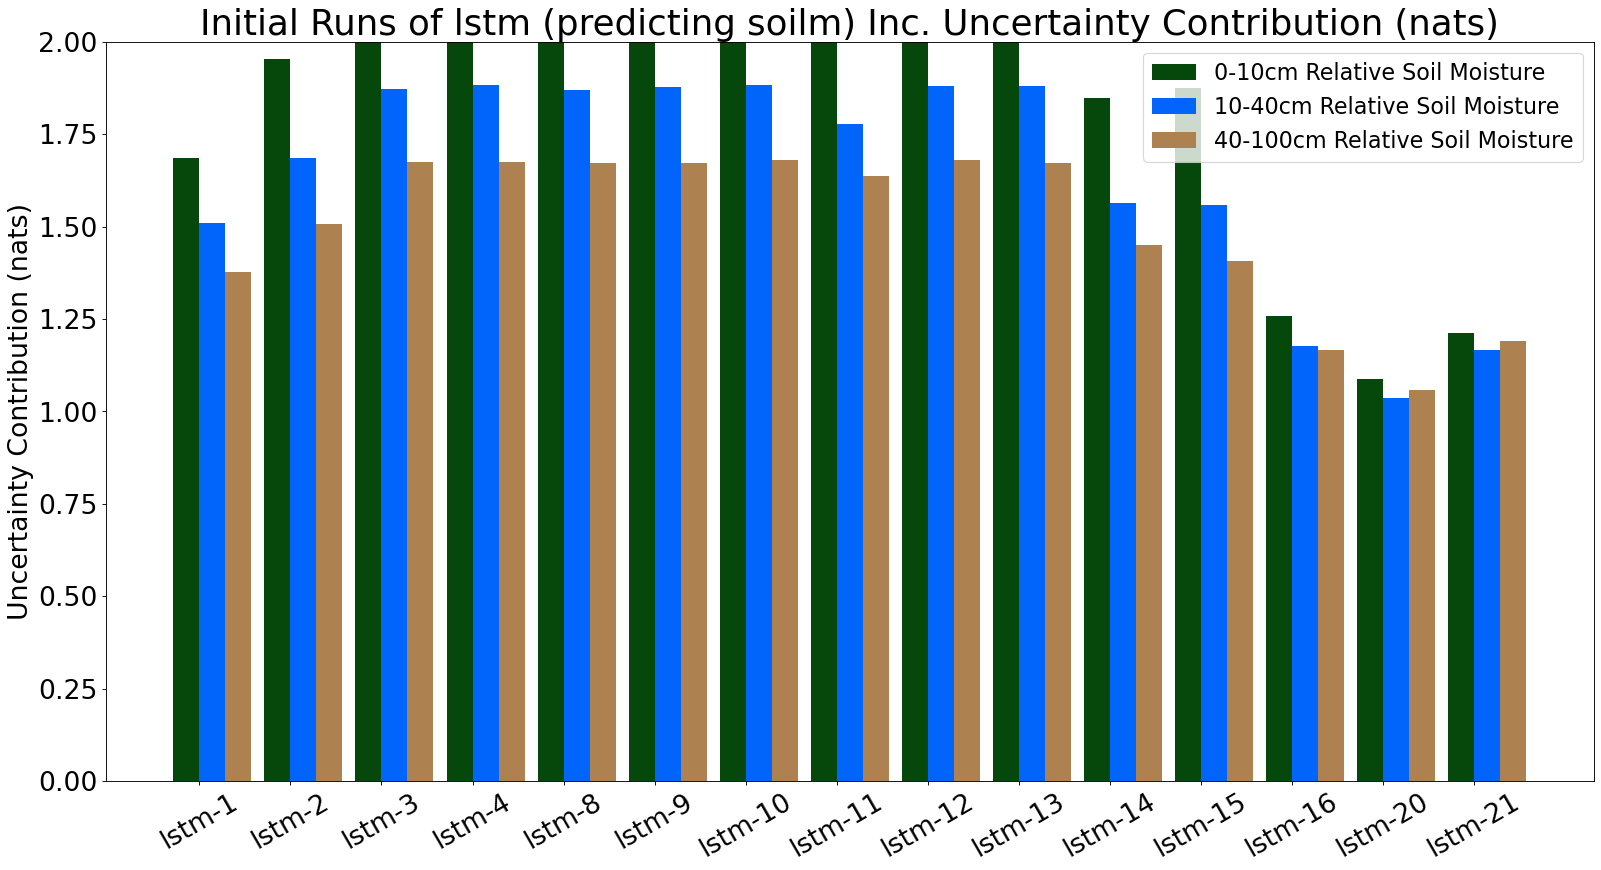
\includegraphics[width=.48\linewidth,draft=false]{figures/efficiency_initial-best/eval_test_efficiency_initial-lstm-soilm_info-loss_res.png}
    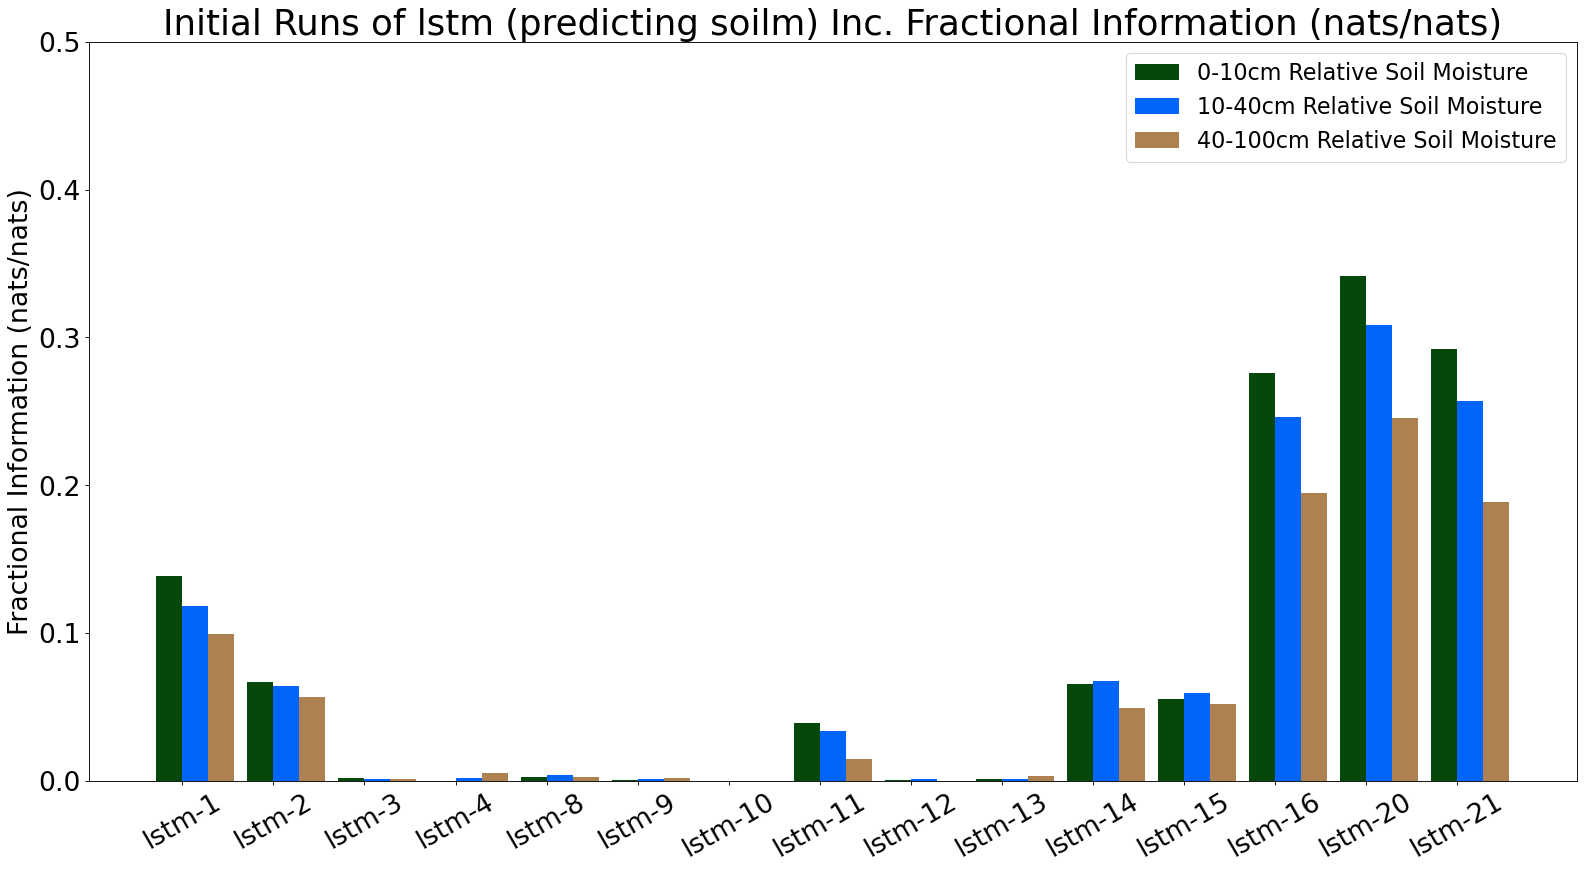
\includegraphics[width=.48\linewidth,draft=false]{figures/efficiency_initial-best/eval_test_efficiency_initial-lstm-soilm_fi_res.png}

    \caption{Bulk metrics for initial LSTM-VSM training runs}
    \label{model-init-fnn}
\end{figure}

\begin{table}[h!p]
    \footnotesize
    \centering
\begin{sideways}
    \begin{tabular}{c|c|c|c|c|c|c }
Name & Desc & Weights & \thead{State\\MAE} & \thead{State\\CC} & \thead{Info\\Loss} &\thead{Frac.\\Info}\\
\hline
\multirow{3}{6em}{lstm-1} & \multirow{3}{16em}{4 layers, 64 wide. No batchnorm. } & \multirow{3}{4em}{254397} & 0.107 & 0.509 & 1.686 & 0.138 \\ & & & 0.039 & 0.612 & 1.509 & 0.118 \\ & & & 0.015 & 0.574 & 1.378 & 0.099 \\
\hline
\multirow{3}{6em}{lstm-2} & \multirow{3}{16em}{batchnorm, higher learning rate} & \multirow{3}{4em}{254397} & 0.074 & 0.450 & 1.954 & 0.067 \\ & & & 0.033 & 0.544 & 1.684 & 0.065 \\ & & & 0.020 & 0.360 & 1.507 & 0.057 \\
\hline
\multirow{3}{6em}{lstm-3} & \multirow{3}{16em}{Slower LR ; much 24 wide and 6 layers deep} & \multirow{3}{4em}{64189} & 2.877 & -0.029 & 2.183 & 0.002 \\ & & & 3.153 & -0.084 & 1.873 & 0.002 \\ & & & 0.783 & 0.107 & 1.675 & 0.002 \\
\hline
\multirow{3}{6em}{lstm-4} & \multirow{3}{16em}{4 layers, 96 wide. faster LR, small loss from state magnitude} & \multirow{3}{4em}{629021} & 0.064 & 0.132 & 2.198 & 0.000 \\ & & & 0.049 & 0.196 & 1.882 & 0.002 \\ & & & 0.022 & 0.205 & 1.675 & 0.006 \\
\hline
\multirow{3}{6em}{lstm-8} & \multirow{3}{16em}{4 layers, 64 wide. bigger batch size} & \multirow{3}{4em}{288829} & 0.095 & 0.077 & 2.188 & 0.003 \\ & & & 0.046 & 0.111 & 1.870 & 0.004 \\ & & & 0.029 & -0.034 & 1.671 & 0.003 \\
\hline
\multirow{3}{6em}{lstm-9} & \multirow{3}{16em}{4 layers, 16 wide. bigger batch size} & \multirow{3}{4em}{20029} & 0.076 & 0.035 & 2.195 & 0.000 \\ & & & 0.046 & -0.064 & 1.877 & 0.001 \\ & & & 0.027 & 0.061 & 1.673 & 0.002 \\
\hline
\multirow{3}{6em}{lstm-10} & \multirow{3}{16em}{6 layers, 24 wide; cyclical learning rate ; higher dropout} & \multirow{3}{4em}{65445} & 0.057 & 0.133 & 2.197 & 0.000 \\ & & & 0.034 & 0.127 & 1.882 & 0.000 \\ & & & 0.020 & 0.016 & 1.680 & 0.000 \\
\hline
\multirow{3}{6em}{lstm-11} & \multirow{3}{16em}{2 layers, 256 wide; slower learning rate} & \multirow{3}{4em}{1929597} & 0.066 & 0.286 & 2.058 & 0.039 \\ & & & 0.032 & 0.534 & 1.779 & 0.034 \\ & & & 0.021 & 0.463 & 1.636 & 0.015 \\
\hline
\multirow{3}{6em}{lstm-12} & \multirow{3}{16em}{4 layers, 32 wide; no batchnorm} & \multirow{3}{4em}{74813} & 0.057 & 0.112 & 2.195 & 0.000 \\ & & & 0.037 & -0.193 & 1.880 & 0.001 \\ & & & 0.023 & -0.193 & 1.679 & 0.000 \\
\hline
\multirow{3}{6em}{lstm-13} & \multirow{3}{16em}{same as lstm-12 but increment ratio .8} & \multirow{3}{4em}{74813} & 0.057 & 0.058 & 2.192 & 0.002 \\ & & & 0.034 & 0.055 & 1.879 & 0.001 \\ & & & 0.020 & 0.055 & 1.671 & 0.003 \\
    \end{tabular}
\end{sideways}
    \caption{Initial LSTM-VSM properties and bulk statistics (1).}
    \label{model-init-lstm-table-1}
\end{table}

\begin{table}[h!p]
    \footnotesize
    \centering
\begin{sideways}
    \begin{tabular}{c|c|c|c|c|c|c }
Name & Desc & Weights & \thead{State\\MAE} & \thead{State\\CC} & \thead{Info\\Loss} &\thead{Frac.\\Info}\\
\hline
\multirow{3}{6em}{lstm-14} & \multirow{3}{16em}{Heavy increment error ; decaying log-cyclical learning rate; batch norm} & \multirow{3}{4em}{74813} & 0.726 & 0.357 & 1.847 & 0.065 \\ & & & 0.224 & 0.416 & 1.565 & 0.067 \\ & & & 0.147 & 0.405 & 1.451 & 0.050 \\
\hline
\multirow{3}{6em}{lstm-15} & \multirow{3}{16em}{No dropout, some increment magnitude bias} & \multirow{3}{4em}{74813} & 1.556 & 0.385 & 1.874 & 0.055 \\ & & & 1.481 & 0.385 & 1.558 & 0.060 \\ & & & 0.831 & 0.352 & 1.407 & 0.052 \\
\hline
\multirow{3}{6em}{lstm-16} & \multirow{3}{16em}{Same as lstm-15 but smaller learning rate} & \multirow{3}{4em}{74813} & 0.032 & 0.826 & 1.258 & 0.276 \\ & & & 0.017 & 0.779 & 1.176 & 0.246 \\ & & & 0.010 & 0.754 & 1.166 & 0.195 \\
\hline
\multirow{3}{6em}{lstm-20} & \multirow{3}{16em}{Stronger dependence on state, some increment magnitude bias, dropout} & \multirow{3}{4em}{77117} & 0.021 & 0.882 & 1.088 & 0.342 \\ & & & 0.013 & 0.884 & 1.036 & 0.309 \\ & & & 0.008 & 0.842 & 1.058 & 0.246 \\
\hline
\multirow{3}{6em}{lstm-21} & \multirow{3}{16em}{lstm-20 but more dropout, more increment magnitude bias, some state loss} & \multirow{3}{4em}{77117} & 0.025 & 0.866 & 1.213 & 0.292 \\ & & & 0.016 & 0.833 & 1.166 & 0.257 \\ & & & 0.011 & 0.762 & 1.191 & 0.189 \\
\hline
\multirow{3}{6em}{lstm-22} & \multirow{3}{16em}{4 layers, 32 wide, faster learning rate} & \multirow{3}{4em}{80221} & 0.035 & 0.823 &  &  \\ & & & 0.020 & 0.816 &  &  \\ & & & 0.013 & 0.737 &  &  \\
\hline
\multirow{3}{6em}{lstm-23} & \multirow{3}{16em}{much smaller encoder, heavier on increment, but less magnitude bias} & \multirow{3}{4em}{43597} & 0.034 & 0.835 &  &  \\ & & & 0.019 & 0.838 &  &  \\ & & & 0.013 & 0.756 &  &  \\
\hline
\multirow{3}{6em}{lstm-24} & \multirow{3}{16em}{64 nodes wide, 5 layers deep; weaker dependence on increment, strong increment magnitude bias} & \multirow{3}{4em}{173165} & 0.035 & 0.821 &  &  \\ & & & 0.018 & 0.840 &  &  \\ & & & 0.013 & 0.735 &  &  \\
\hline
\multirow{3}{6em}{lstm-25} & \multirow{3}{16em}{Same as lstm-24, but 128 nodes wide} & \multirow{3}{4em}{364029} & 0.035 & 0.823 &  &  \\ & & & 0.019 & 0.829 &  &  \\ & & & 0.012 & 0.754 &  &  \\
\hline
\multirow{3}{6em}{lstm-26} & \multirow{3}{16em}{Same as lstm-25, 6 layers deep} & \multirow{3}{4em}{762413} & 0.050 & 0.712 &  &  \\ & & & 0.026 & 0.732 &  &  \\ & & & 0.015 & 0.658 &  &  \\
\hline
\multirow{3}{6em}{lstm-27} & \multirow{3}{16em}{Same as lstm-24, more increment error} & \multirow{3}{4em}{173165} & 0.037 & 0.822 &  &  \\ & & & 0.019 & 0.848 &  &  \\ & & & 0.012 & 0.754 &  &  \\
    \end{tabular}
\end{sideways}
    \caption{Initial LSTM-VSM properties and bulk statistics (2).}
    \label{model-init-lstm-table-2}
\end{table}

Next, we present a variety of LSTM instances that predict the increment change in volumetric soil moisture (VSM; $\frac{kg}{m^2}$), which we will refer to as the LSTM-VSM group. The results reported here have been converted to relative soil moisture after-the-fact for consistency with the other architectures. In practice, these were the first generations of models we tested; those which appear in Table \ref{model-init-lstm-table-1} were trained using a consistent learning rate and converged rapidly to fairly poor results. Even relatively large models with a variety of hyperparameter configurations didn't achieve a correlation coefficient higher than .65 for any of the layers. Introducing the log-cyclical learning rate schedule prolonged training and, combined with the loss function modifications, resulted in considerably better-performing LSTMs. Given its apparent success, we continued to use the log-cyclical learning rate strategy for the remainder of the models, changing only the rate of decay and the initial minima and maxima of the oscillations. The best LSTM-VSM models we trained had 77,117 trainable weights, a magnitude bias parameter of $\gamma = 10$, increment loss ratio $\rho = .999$, and did not use increment normalization within the loss function. Unlike the FNN architectures, the best LSTM-VSM variants tended to include a small weight dropout of 5\% during training, however without further analysis it is difficult to draw conclusions on the actual impact of any of these changes in isolation.

\begin{figure}[hp!]
    \centering
    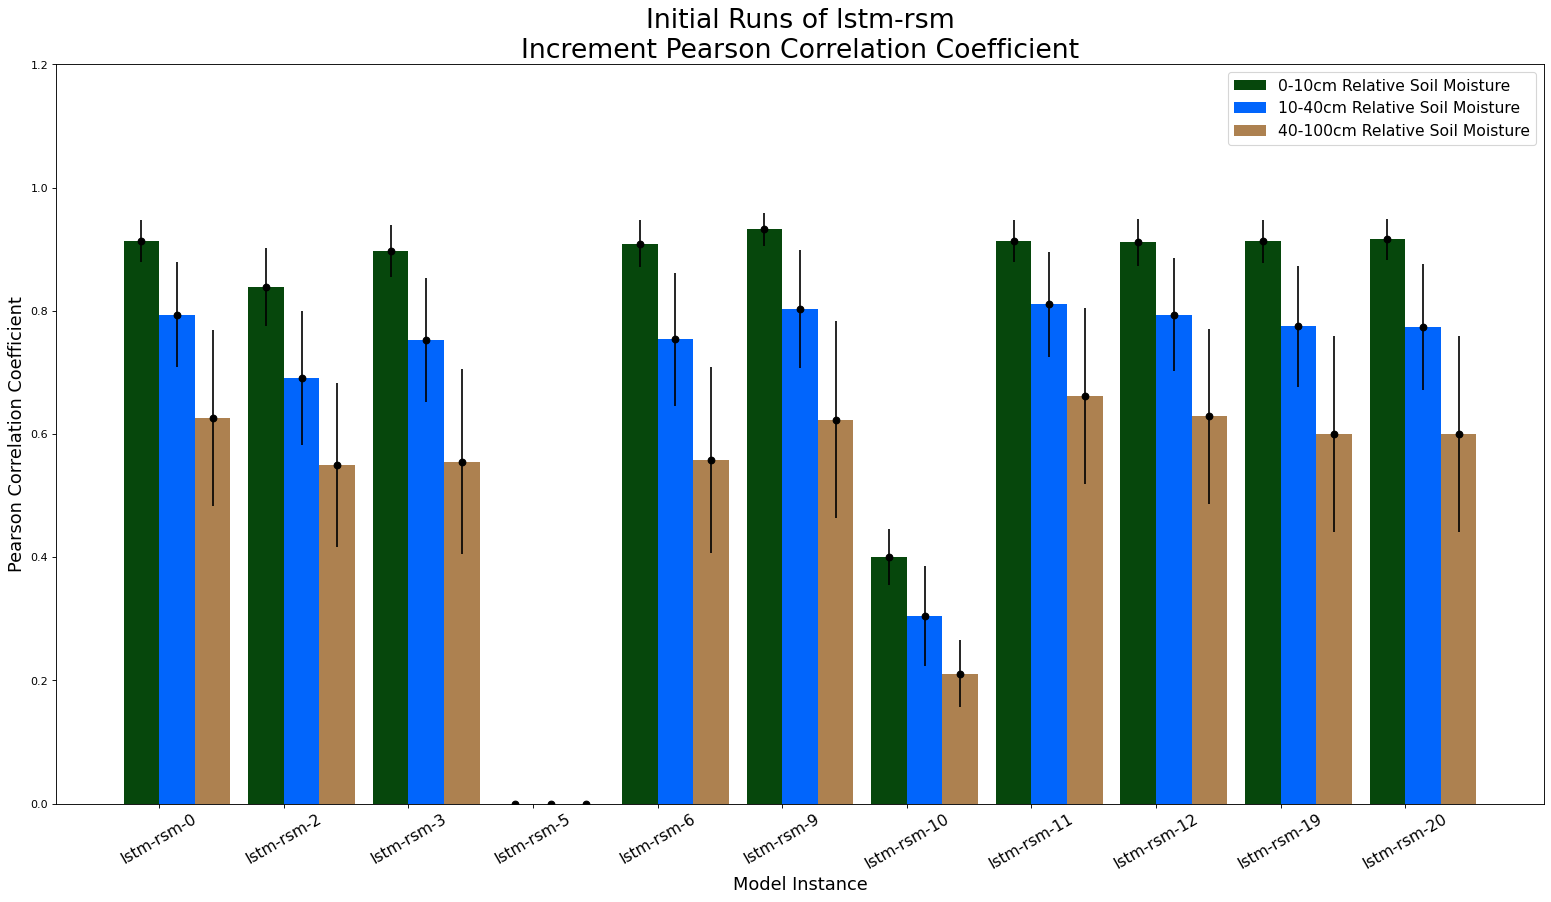
\includegraphics[width=.48\linewidth,draft=false]{figures/efficiency_initial-best/eval_test_efficiency_initial-lstm-rsm_cc_res.png}
    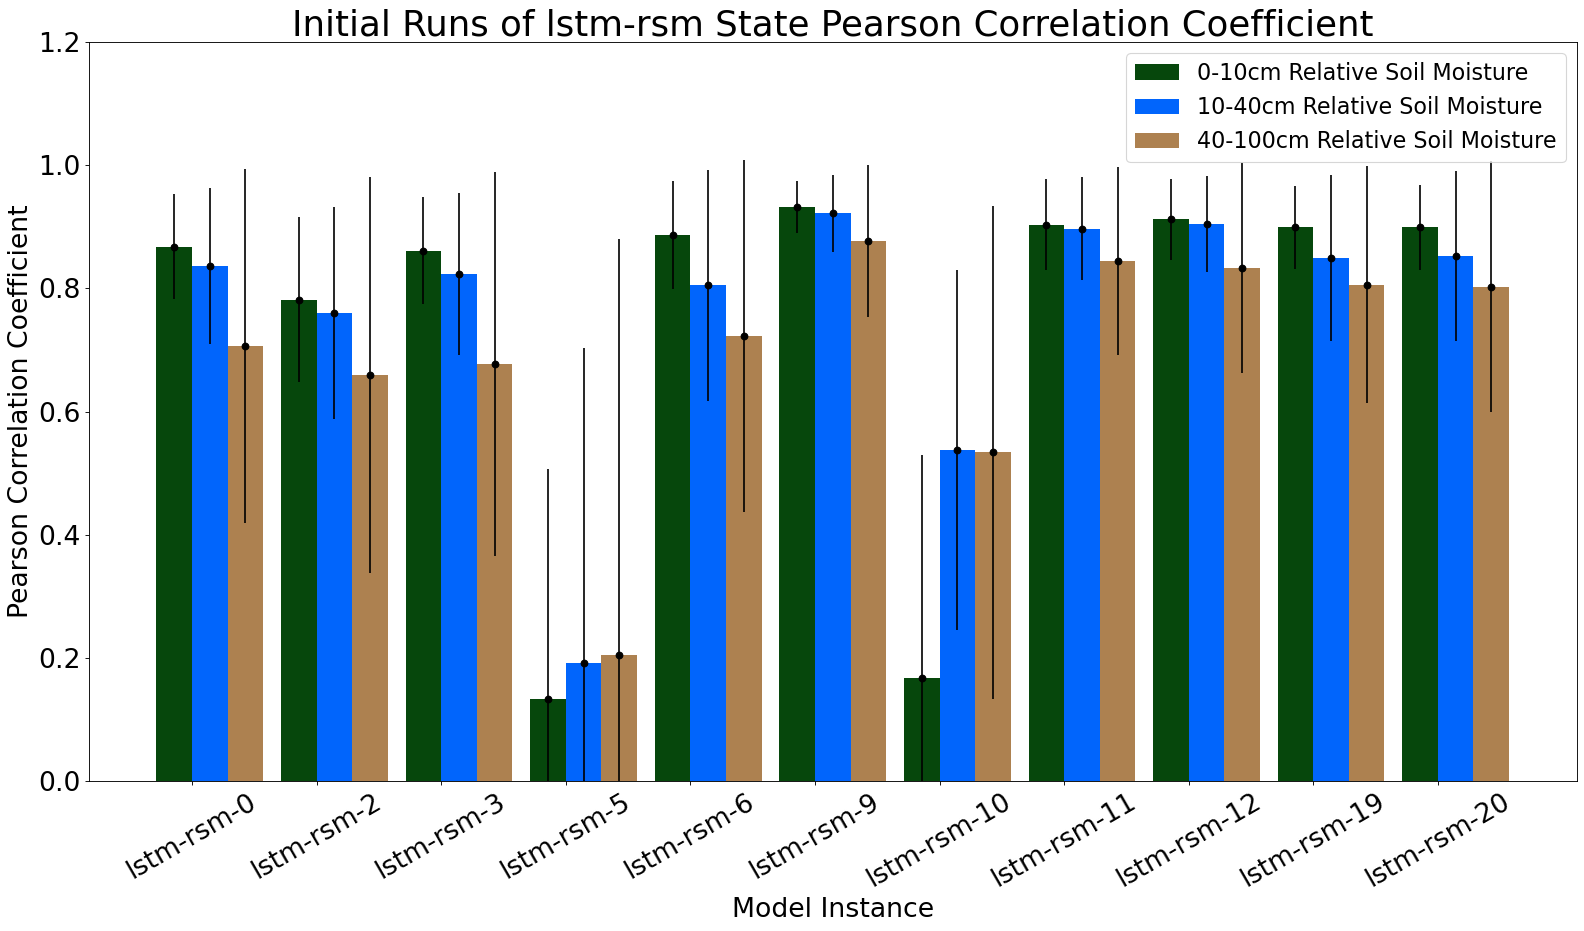
\includegraphics[width=.48\linewidth,draft=false]{figures/efficiency_initial-best/eval_test_efficiency_initial-lstm-rsm_cc_state.png}

    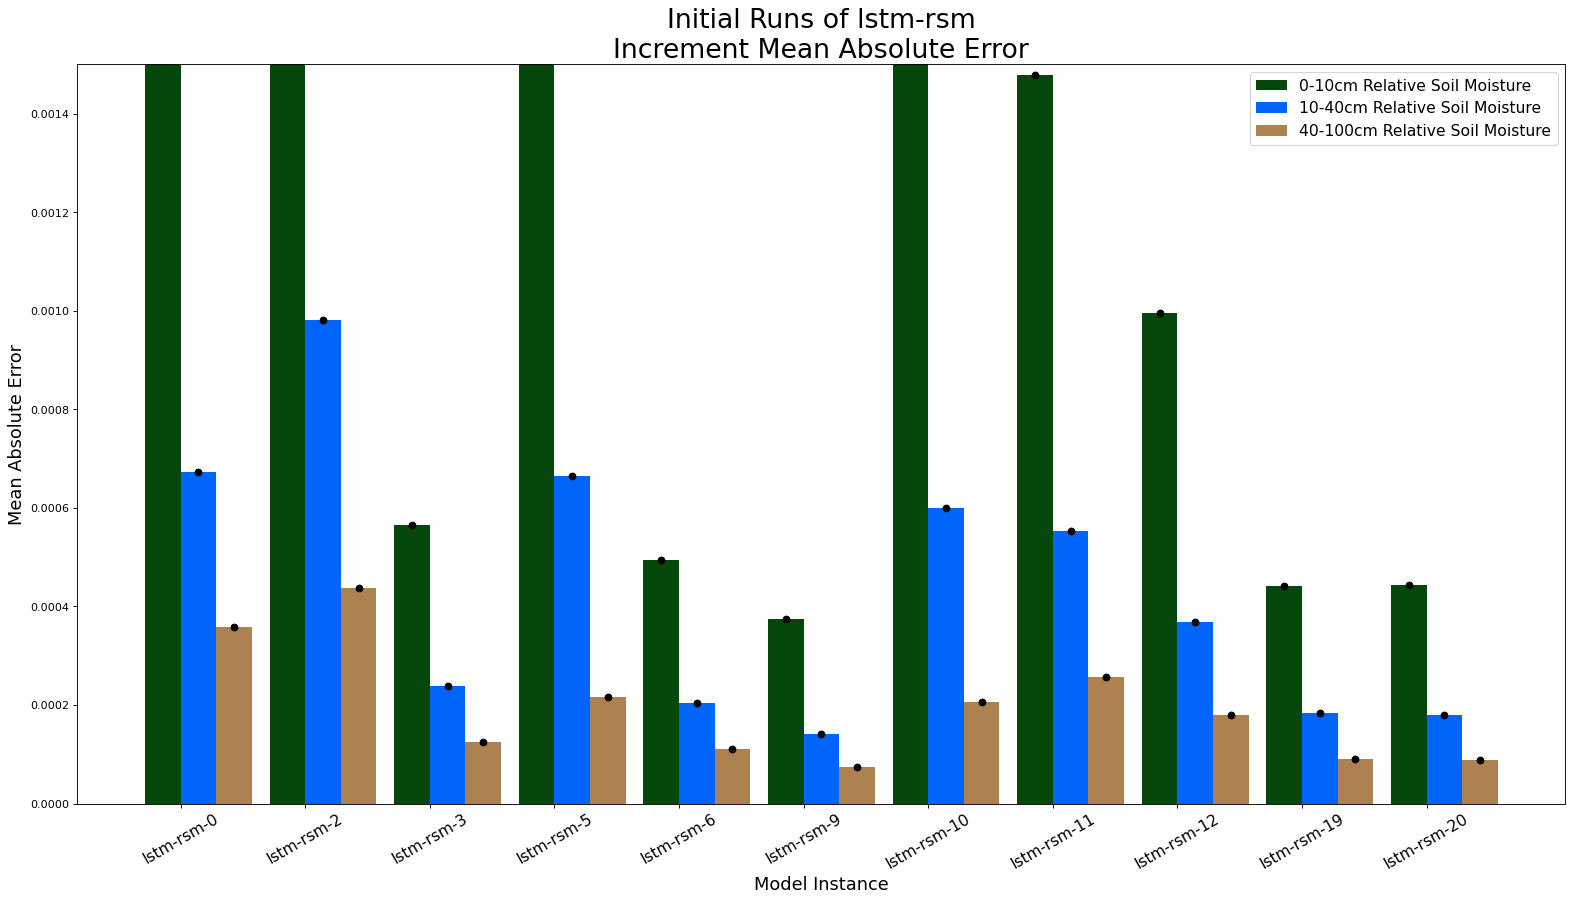
\includegraphics[width=.48\linewidth,draft=false]{figures/efficiency_initial-best/eval_test_efficiency_initial-lstm-rsm_mae_res.png}
    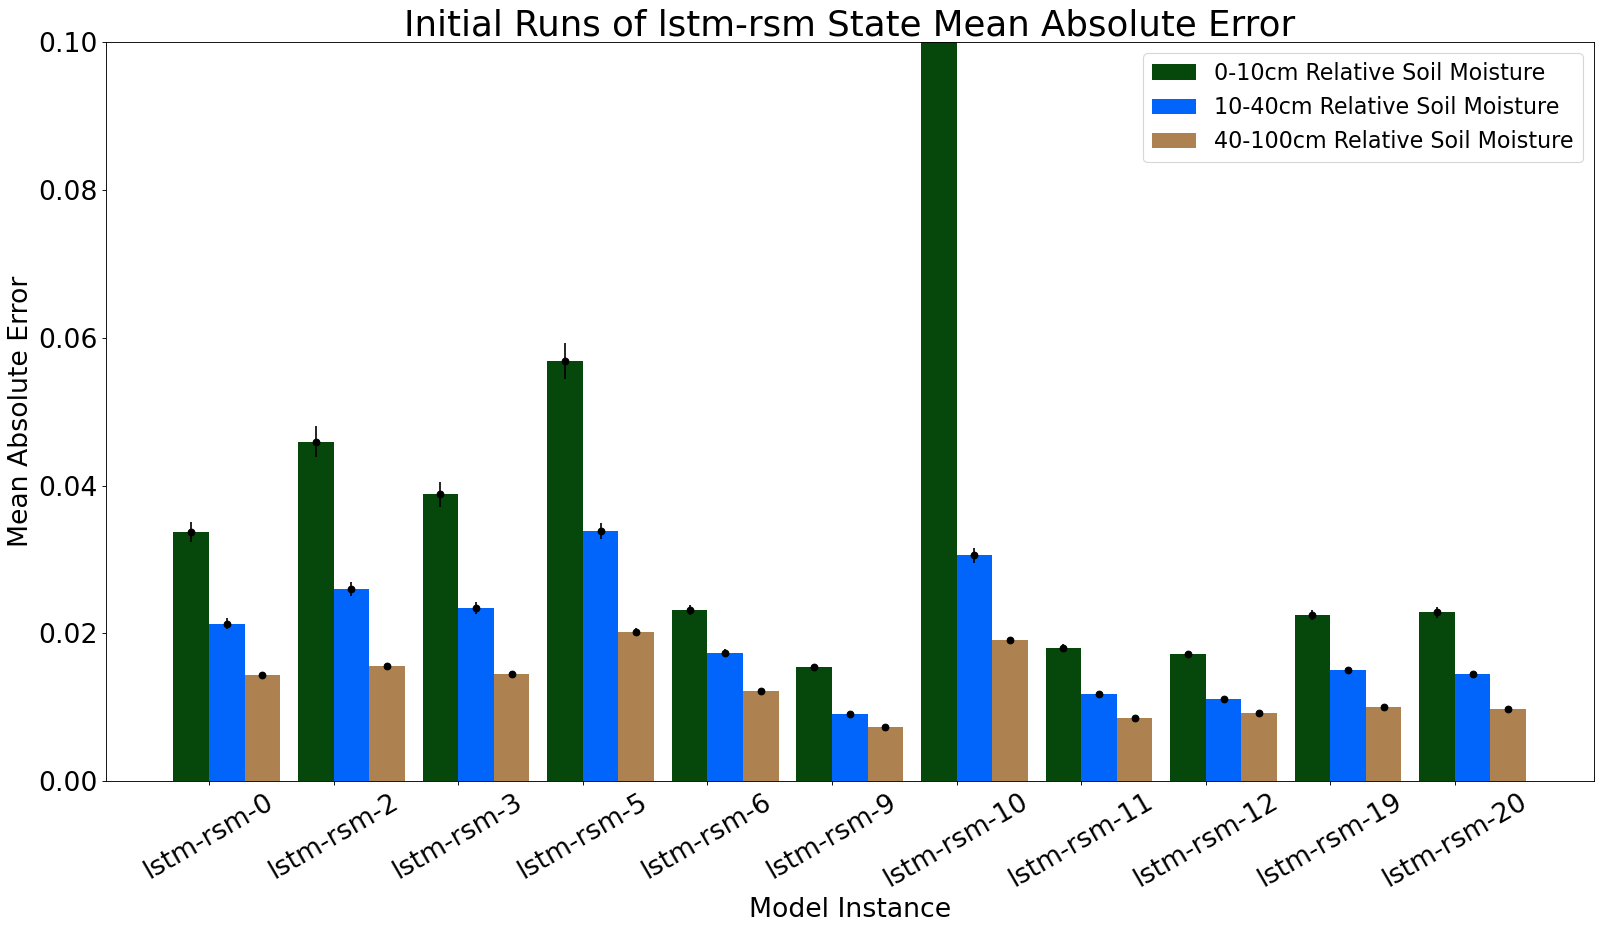
\includegraphics[width=.48\linewidth,draft=false]{figures/efficiency_initial-best/eval_test_efficiency_initial-lstm-rsm_mae_state.png}

    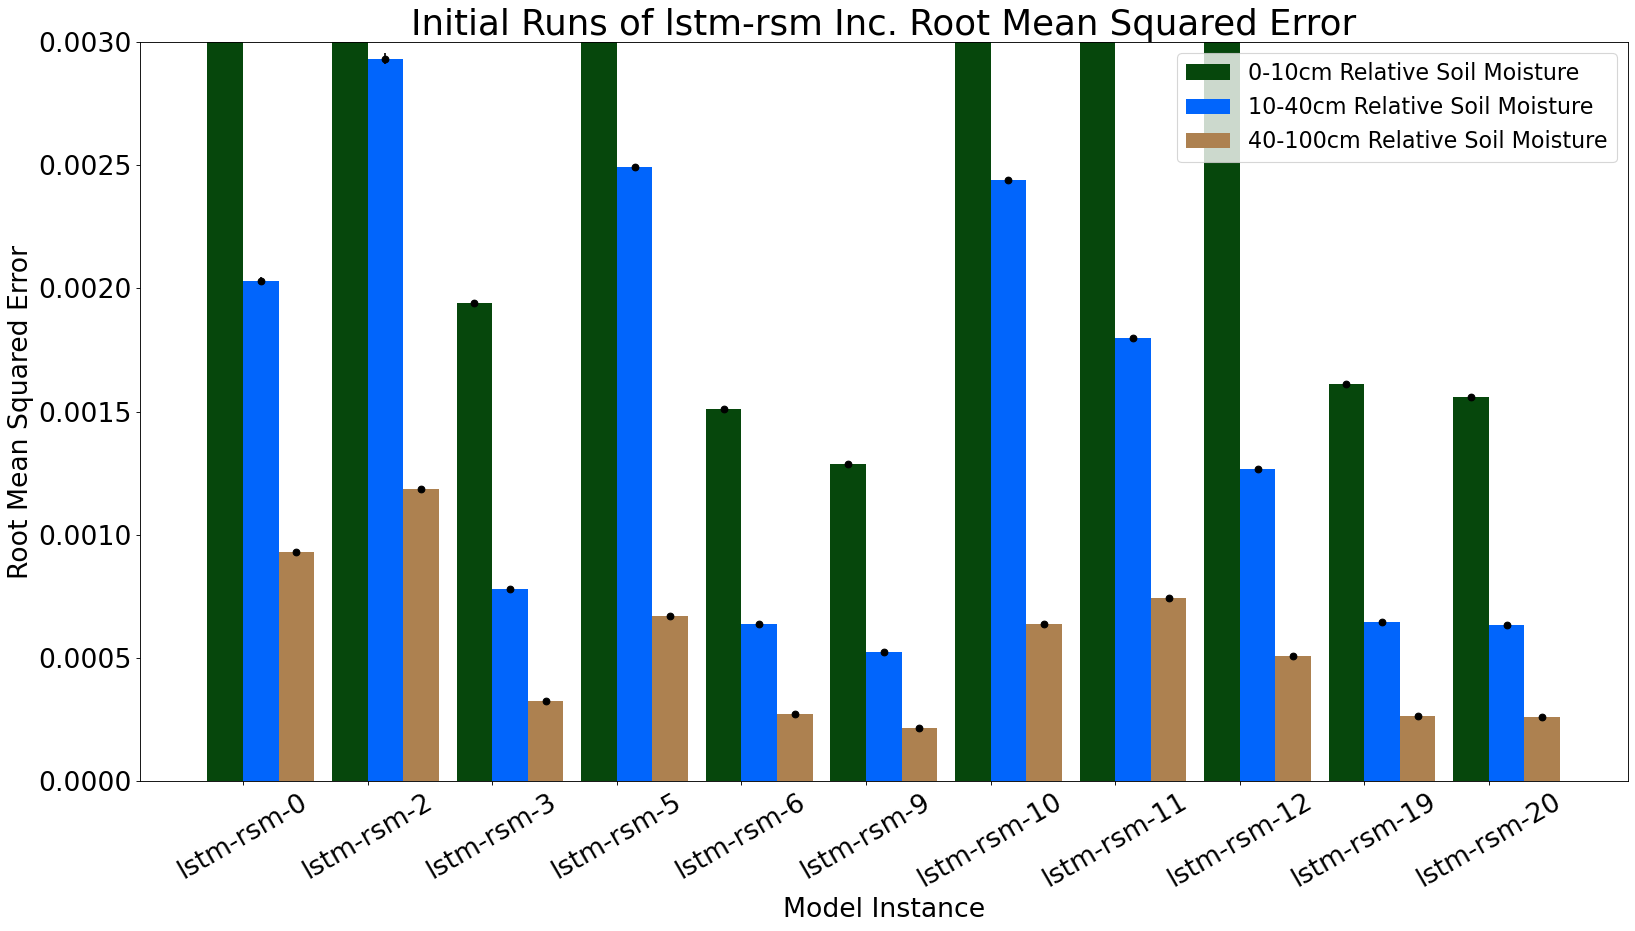
\includegraphics[width=.48\linewidth,draft=false]{figures/efficiency_initial-best/eval_test_efficiency_initial-lstm-rsm_mse_res.png}
    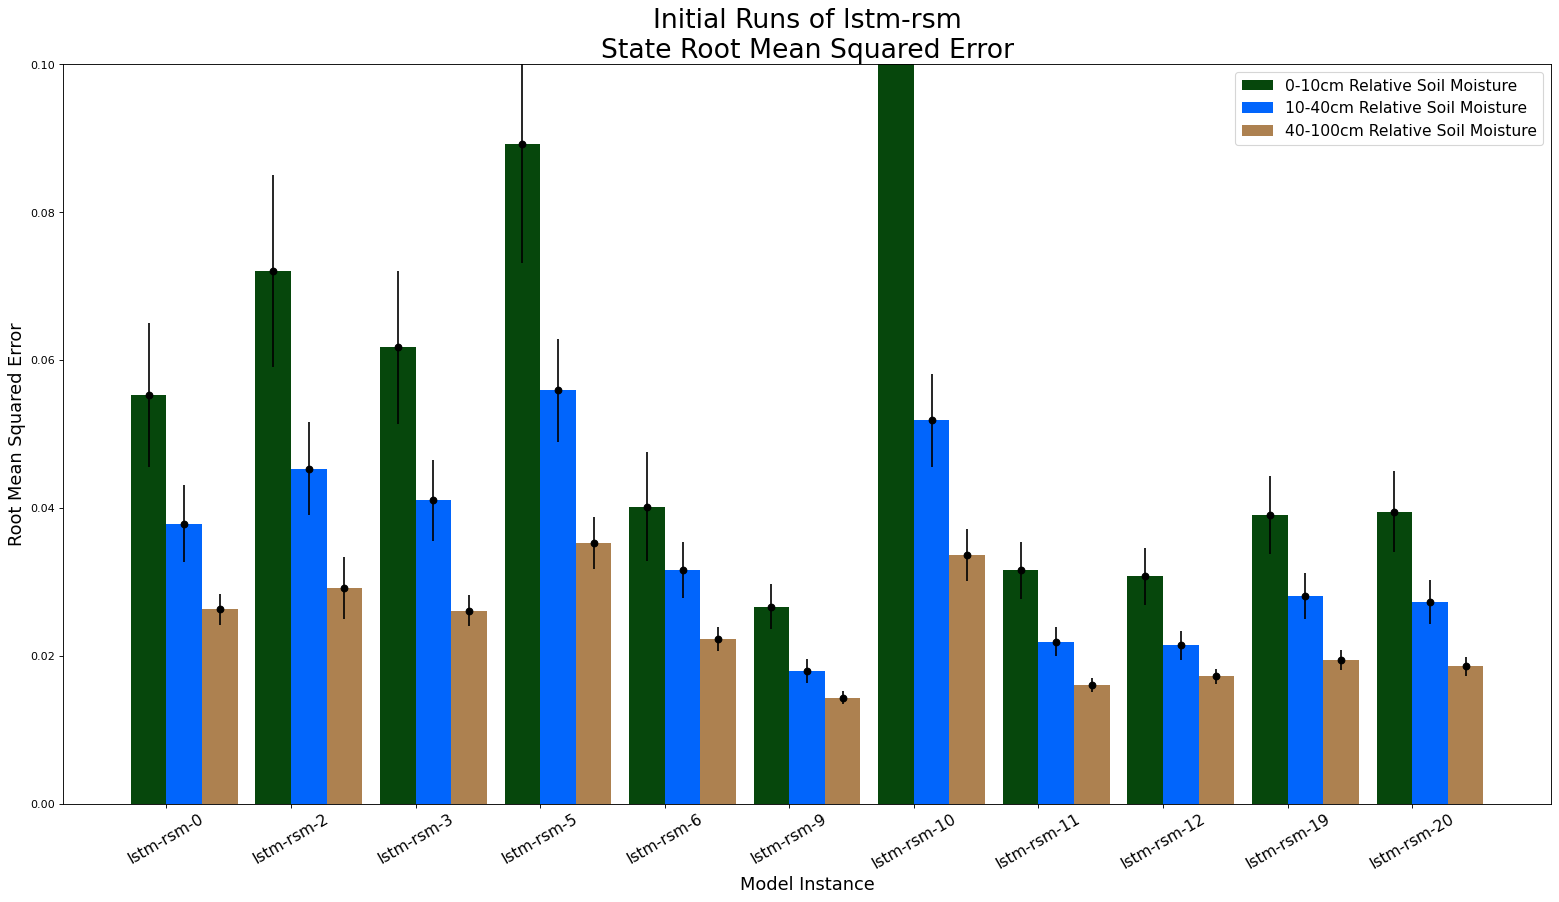
\includegraphics[width=.48\linewidth,draft=false]{figures/efficiency_initial-best/eval_test_efficiency_initial-lstm-rsm_mse_state.png}

    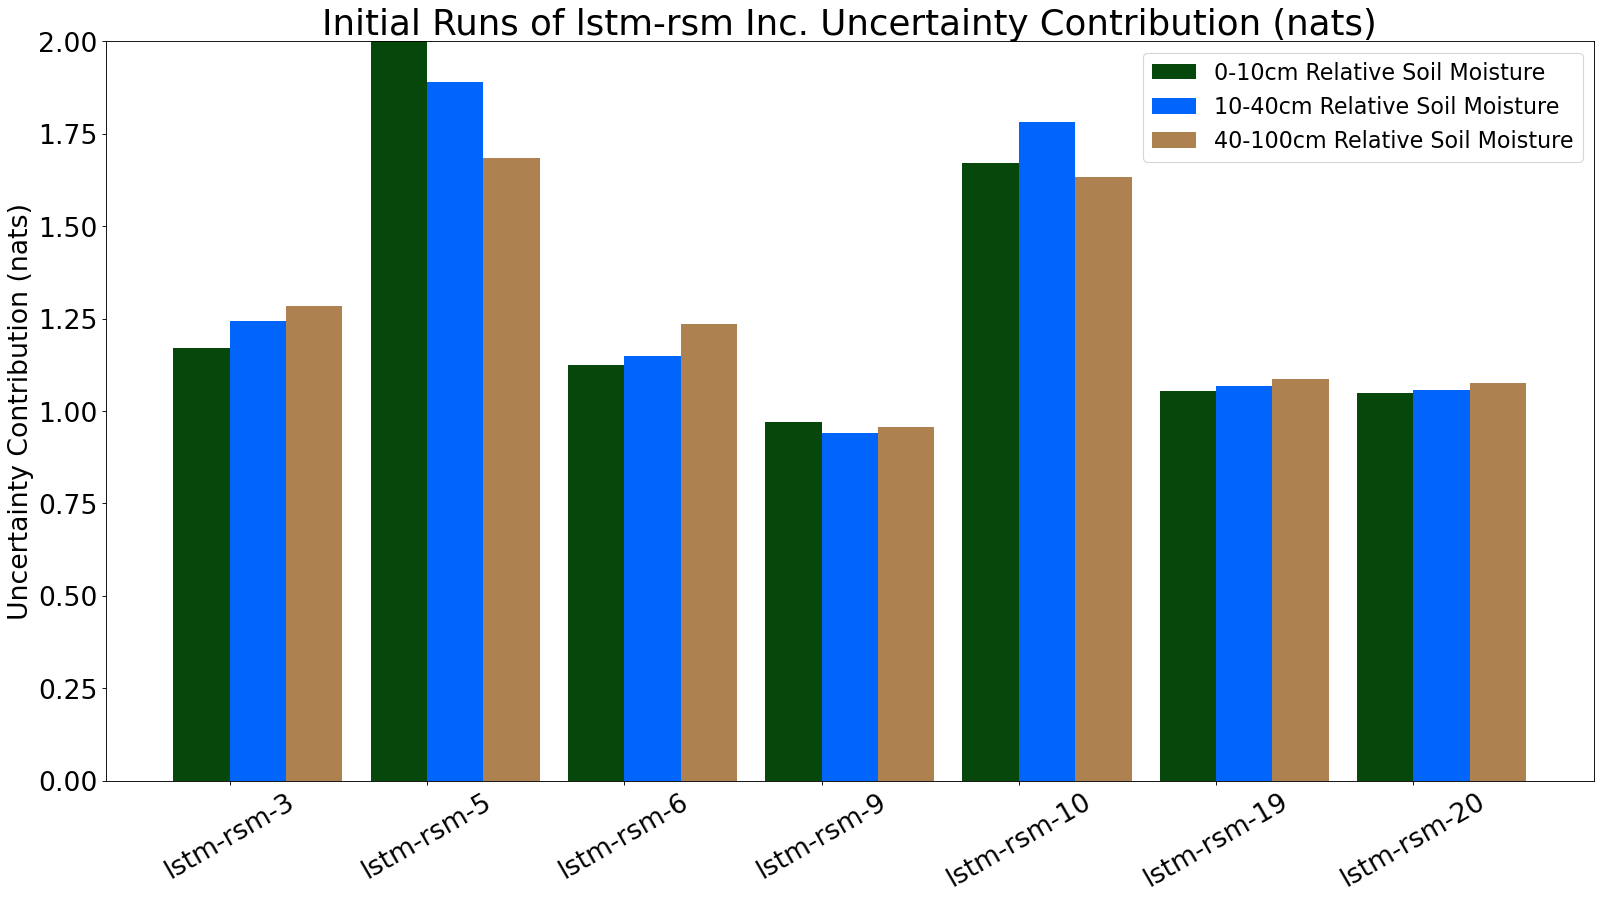
\includegraphics[width=.48\linewidth,draft=false]{figures/efficiency_initial-best/eval_test_efficiency_initial-lstm-rsm_info-loss_res.png}
    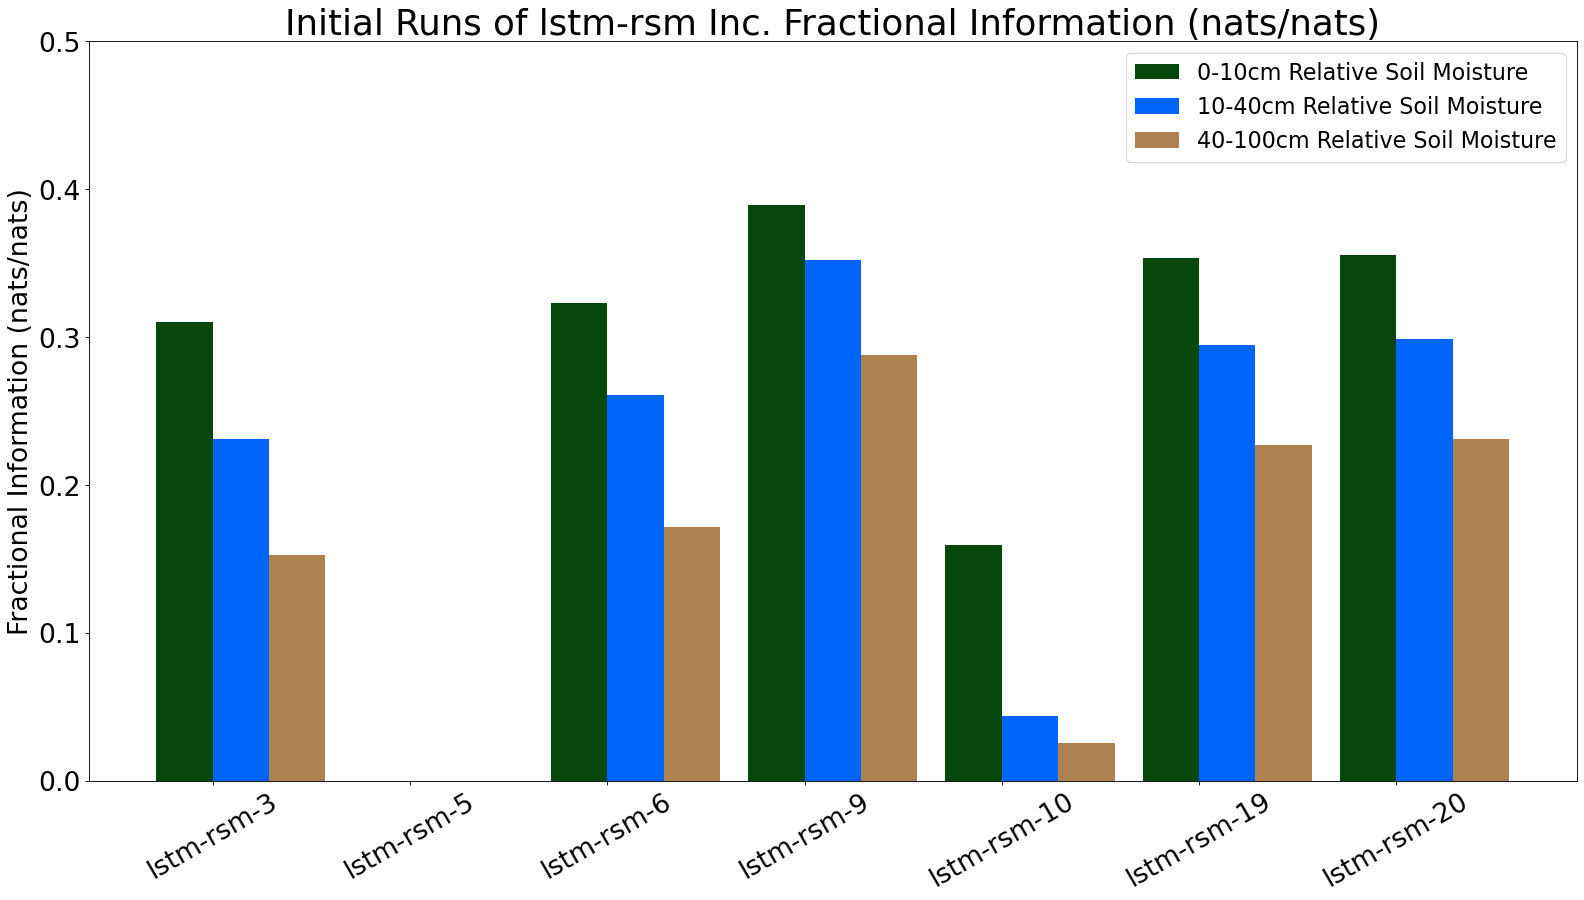
\includegraphics[width=.48\linewidth,draft=false]{figures/efficiency_initial-best/eval_test_efficiency_initial-lstm-rsm_fi_res.png}

    \caption{Bulk metrics for initial LSTM-RSM (relative soil moisture predictor) training runs}
    \label{model-init-lstm-rsm}
\end{figure}

\begin{table}[h!p]
    \footnotesize
    \centering
\begin{sideways}
    \begin{tabular}{c|c|c|c|c|c|c }
Name & Desc & Weights & \thead{State\\MAE} & \thead{State\\CC} & \thead{Info\\Loss} &\thead{Frac.\\Info}\\
\hline
\multirow{3}{6em}{lstm-rsm-0} & \multirow{3}{16em}{Small magnitude bias. low dropout. small batch size. 64-wide 4-layer.} & \multirow{3}{4em}{179483} & 0.034 & 0.868 &  &  \\ & & & 0.021 & 0.837 &  &  \\ & & & 0.014 & 0.707 &  &  \\
\hline
\multirow{3}{6em}{lstm-rsm-2} & \multirow{3}{16em}{same as rsm-1, but some state error influence, magnitude bias 30} & \multirow{3}{4em}{179483} & 0.046 & 0.782 &  &  \\ & & & 0.026 & 0.761 &  &  \\ & & & 0.016 & 0.660 &  &  \\
\hline
\multirow{3}{6em}{lstm-rsm-3} & \multirow{3}{16em}{Low dropout, 4 deep, 64 wide decoder, and increment-only loss} & \multirow{3}{4em}{176379} & 0.039 & 0.861 & 1.169 & 0.310 \\ & & & 0.023 & 0.823 & 1.243 & 0.231 \\ & & & 0.015 & 0.677 & 1.285 & 0.152 \\
\hline
\multirow{3}{6em}{lstm-rsm-5} & \multirow{3}{16em}{Same as lstm-rsm-3, but 10\% state influence in loss function} & \multirow{3}{4em}{176379} & 0.057 & 0.133 & 2.206 & 0.000 \\ & & & 0.034 & 0.191 & 1.890 & 0.000 \\ & & & 0.020 & 0.205 & 1.686 & 0.000 \\
\hline
\multirow{3}{6em}{lstm-rsm-6} & \multirow{3}{16em}{Small 3-layer predictor with 100 increment magnitude bias} & \multirow{3}{4em}{48667} & 0.023 & 0.886 & 1.124 & 0.323 \\ & & & 0.017 & 0.805 & 1.149 & 0.261 \\ & & & 0.012 & 0.723 & 1.235 & 0.171 \\
\hline
\multirow{3}{6em}{lstm-rsm-9} & \multirow{3}{16em}{32 nodes wide, 4 layers deep, 10 increment magnitude bias} & \multirow{3}{4em}{48667} & 0.015 & 0.932 & 0.970 & 0.389 \\ & & & 0.009 & 0.922 & 0.941 & 0.352 \\ & & & 0.007 & 0.877 & 0.958 & 0.288 \\
\hline
\multirow{3}{6em}{lstm-rsm-10} & \multirow{3}{16em}{256 nodes wide 5-layer model} & \multirow{3}{4em}{2614907} & 0.138 & 0.168 & 1.671 & 0.159 \\ & & & 0.031 & 0.537 & 1.783 & 0.044 \\ & & & 0.019 & 0.534 & 1.632 & 0.025 \\
%\multirow{3}{6em}{lstm-rsm-11} & \multirow{3}{16em}{same as rsm-9 except coarsened to 3h predictions} & \multirow{3}{4em}{79675} & 0.018 & 0.904 &  &  \\ & & & 0.012 & 0.897 &  &  \\ & & & 0.009 & 0.844 &  &  \\
\hline
\multirow{3}{6em}{lstm-rsm-12} & \multirow{3}{16em}{4 layers deep, 32 nodes wide, steep learning rate decay} & \multirow{3}{4em}{78651} & 0.017 & 0.912 &  &  \\ & & & 0.011 & 0.904 &  &  \\ & & & 0.009 & 0.833 &  &  \\
\hline
\multirow{3}{6em}{lstm-rsm-19} & \multirow{3}{16em}{Single layer 256 nodes wide} & \multirow{3}{4em}{725627} & 0.022 & 0.899 & 1.055 & 0.353 \\ & & & 0.015 & 0.850 & 1.067 & 0.295 \\ & & & 0.010 & 0.806 & 1.086 & 0.227 \\
\hline
\multirow{3}{6em}{lstm-rsm-20} & \multirow{3}{16em}{Same as rsm-19 except some influence of state error} & \multirow{3}{4em}{725627} & 0.023 & 0.899 & 1.048 & 0.356 \\ & & & 0.014 & 0.852 & 1.058 & 0.299 \\ & & & 0.010 & 0.803 & 1.075 & 0.231 \\
    \end{tabular}
\end{sideways}
    \caption{Initial RSM-normalized LSTM properties and bulk statistics.}
    \label{model-init-lstm-rsm-table}
\end{table}

The next group of models we trained will be referred to as LSTM-RSM models, which have the same structure as the previous set, but target the increment change in RSM rather than volumetric soil moisture. Like the LSTM-VSM models, these seemed to show diminishing returns with model sizes beyond 100,000 weights. The best model we identified has only 48,667 trainable weights, and is 4 layers in depth. Curiously, while the loss function manipulations appeared to have a positive impact on the FNN and LSTM-VSM variants, LSTM-RSM models generally underperformed when a higher magnitude bias and a stronger contribution from the state were used. The best model had a relatively small increment magnitude bias $\gamma=10$, and no contribution from state error ($\rho=1$).


%\begin{figure}[hp!]
%    \centering
%    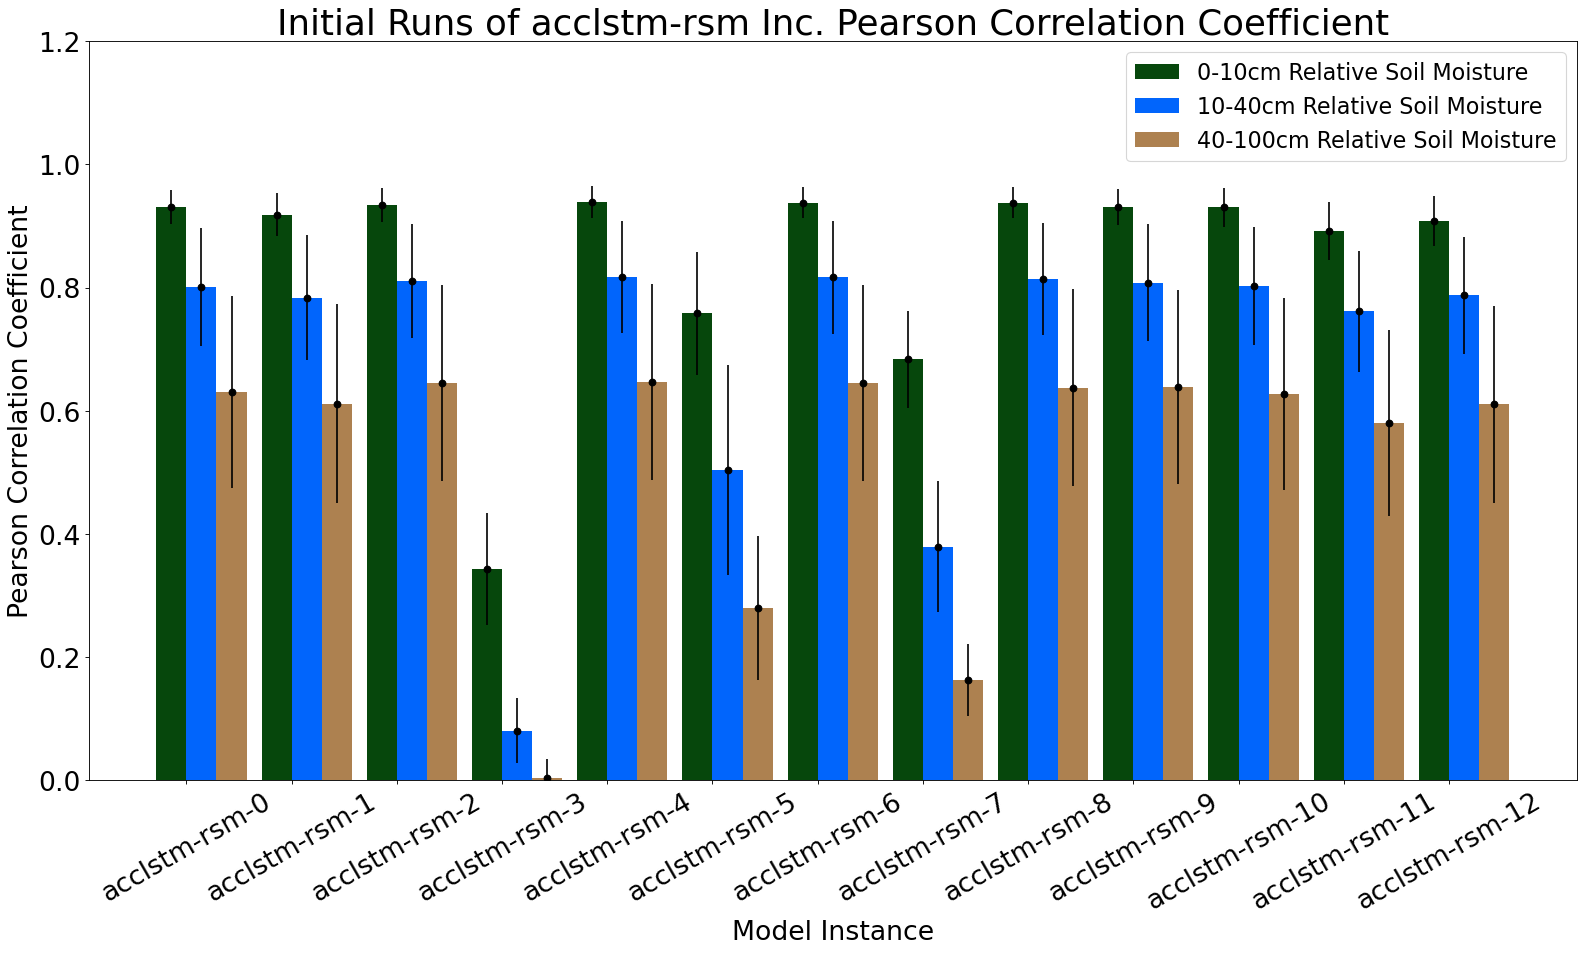
\includegraphics[width=.48\linewidth,draft=false]{figures/efficiency_initial-best/eval_test_efficiency_initial-acclstm-rsm_cc_res.png}
%    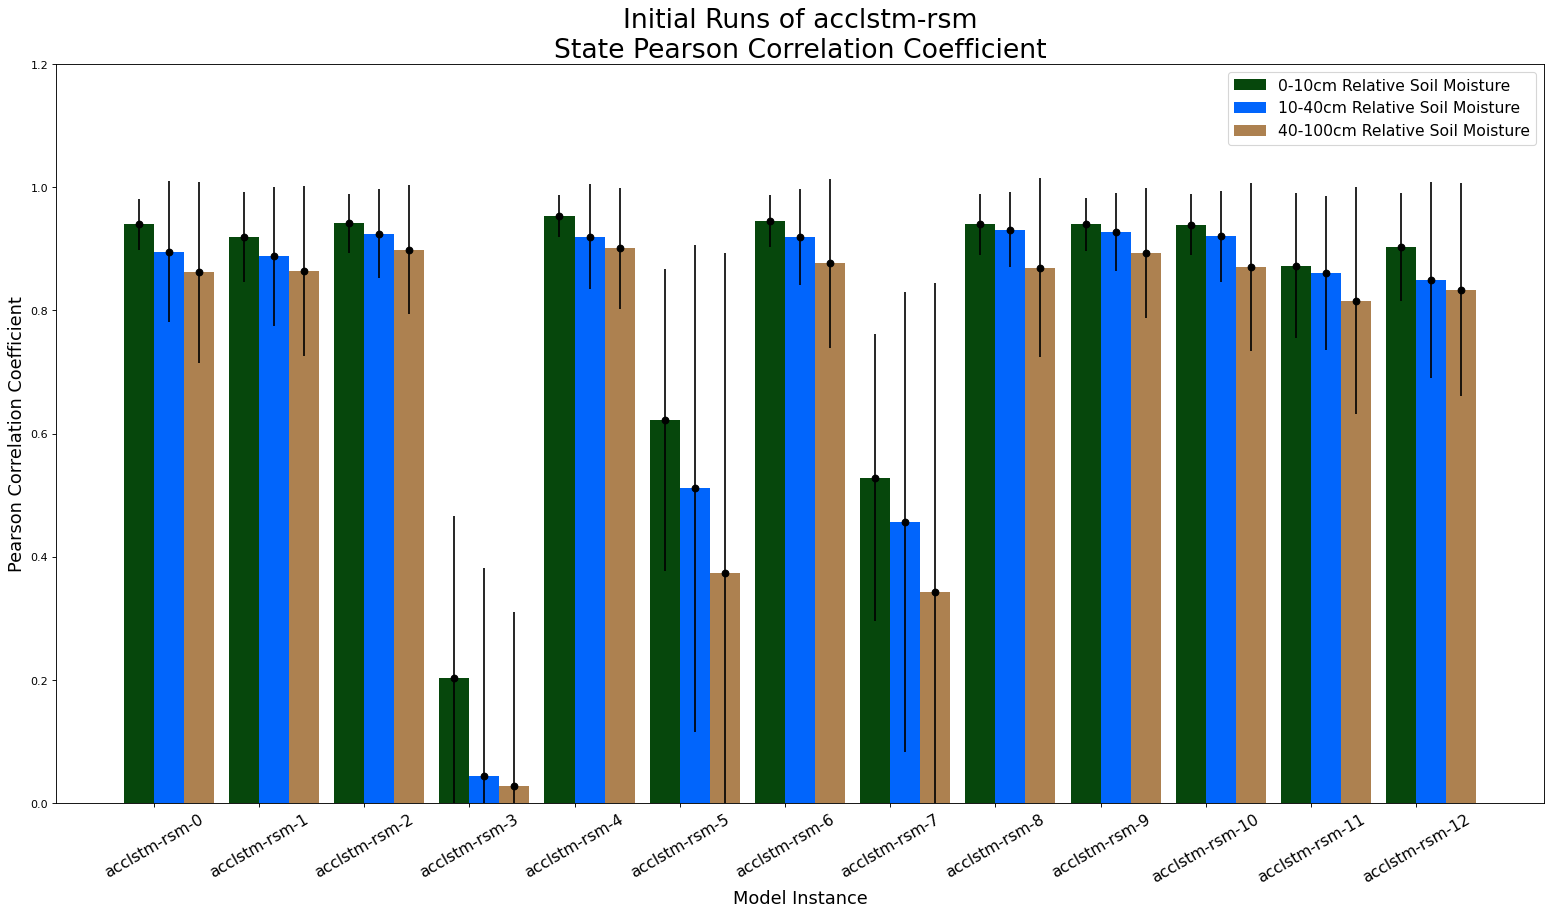
\includegraphics[width=.48\linewidth,draft=false]{figures/efficiency_initial-best/eval_test_efficiency_initial-acclstm-rsm_cc_state.png}
%
%    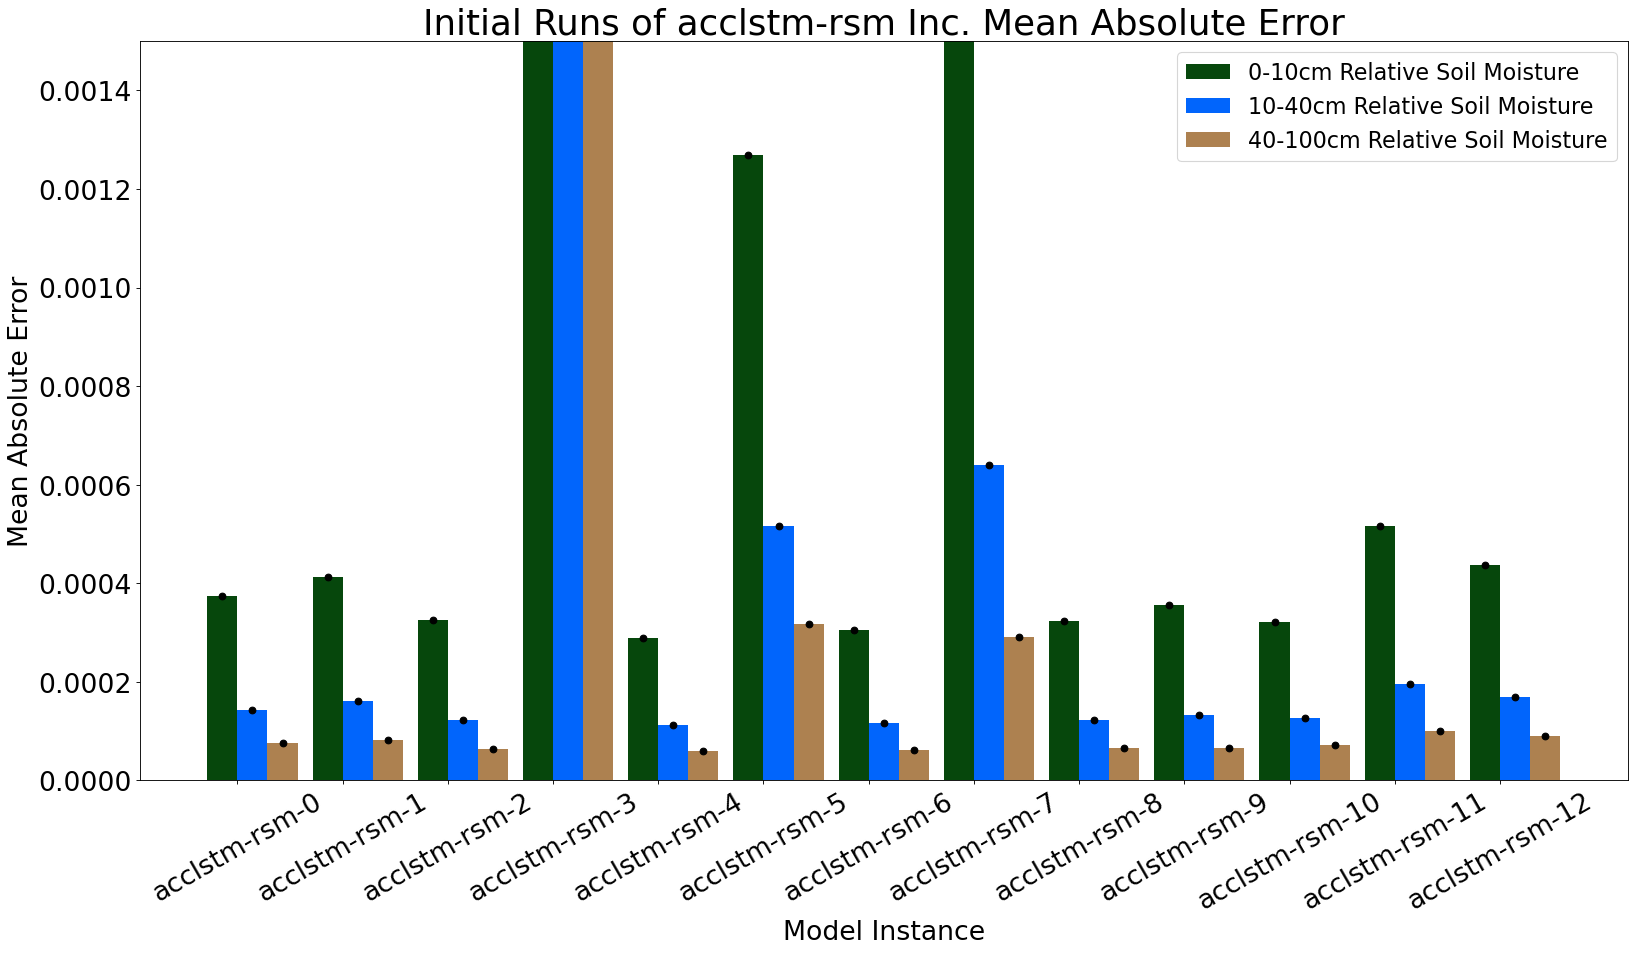
\includegraphics[width=.48\linewidth,draft=false]{figures/efficiency_initial-best/eval_test_efficiency_initial-acclstm-rsm_mae_res.png}
%    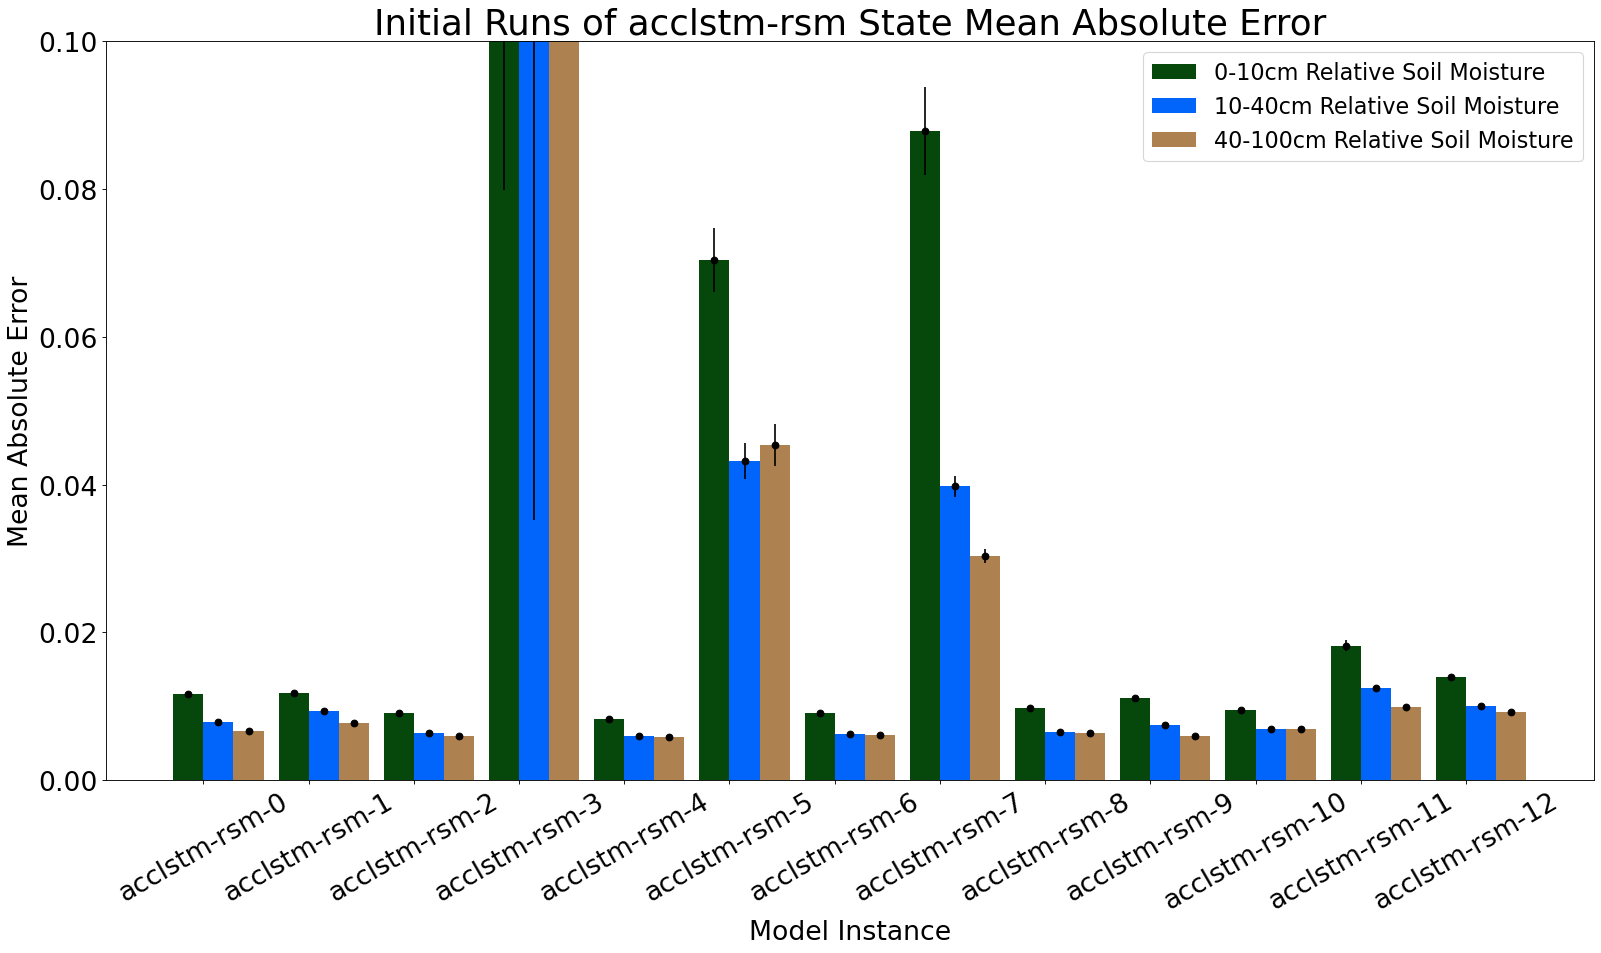
\includegraphics[width=.48\linewidth,draft=false]{figures/efficiency_initial-best/eval_test_efficiency_initial-acclstm-rsm_mae_state.png}
%
%    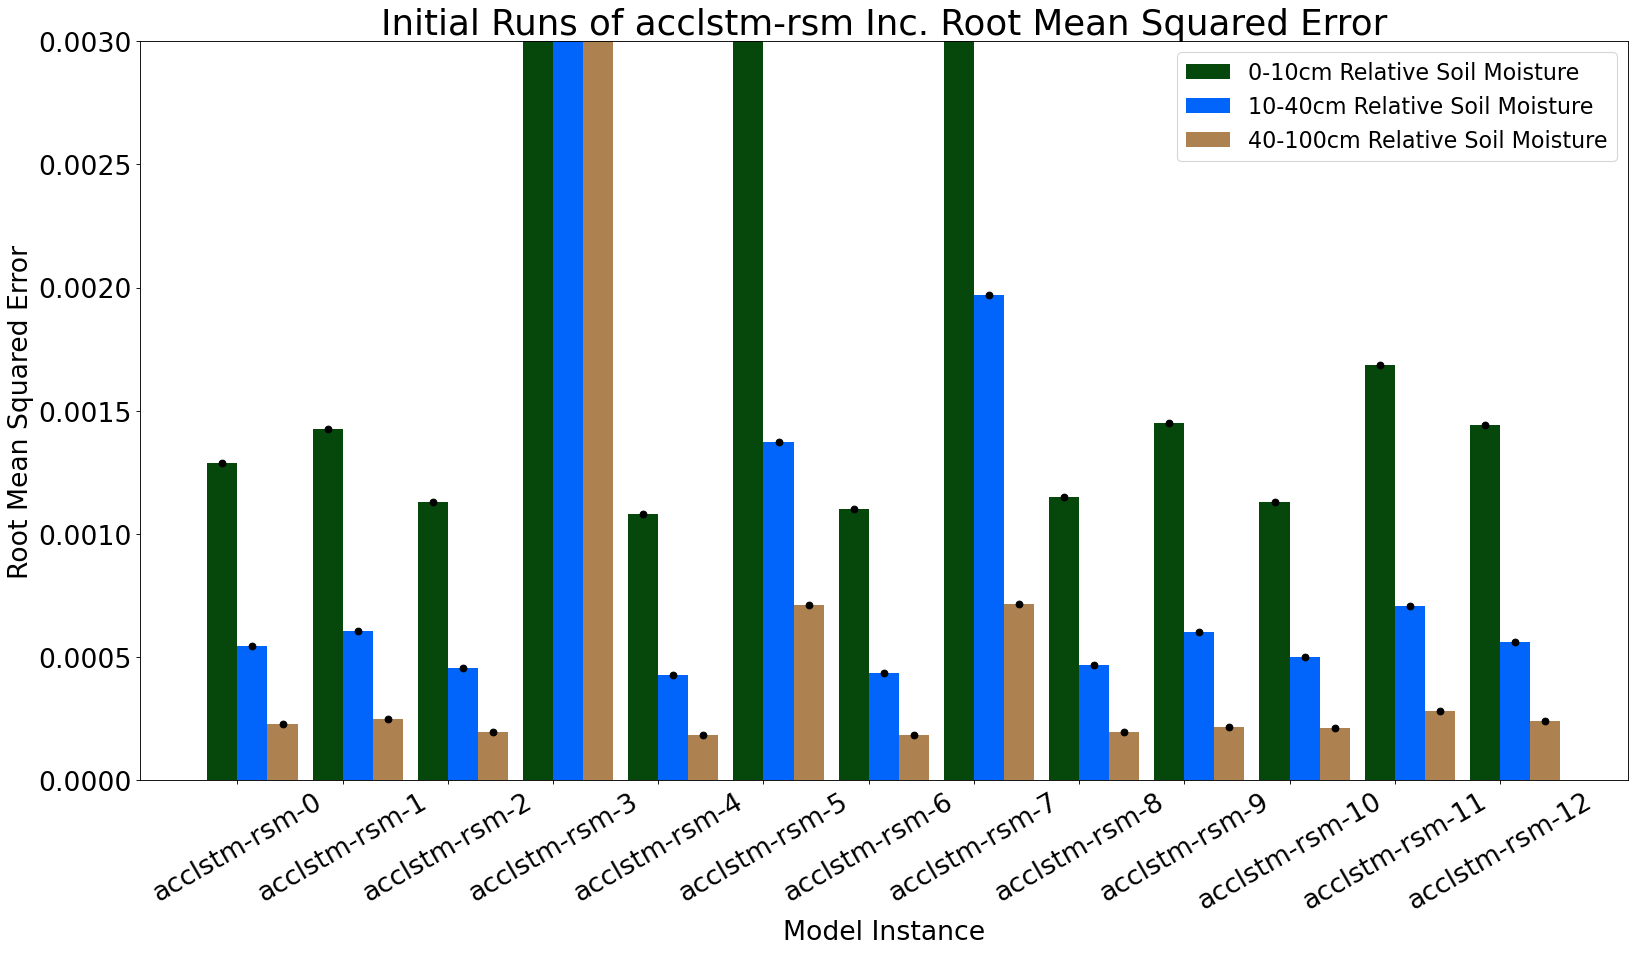
\includegraphics[width=.48\linewidth,draft=false]{figures/efficiency_initial-best/eval_test_efficiency_initial-acclstm-rsm_mse_res.png}
%    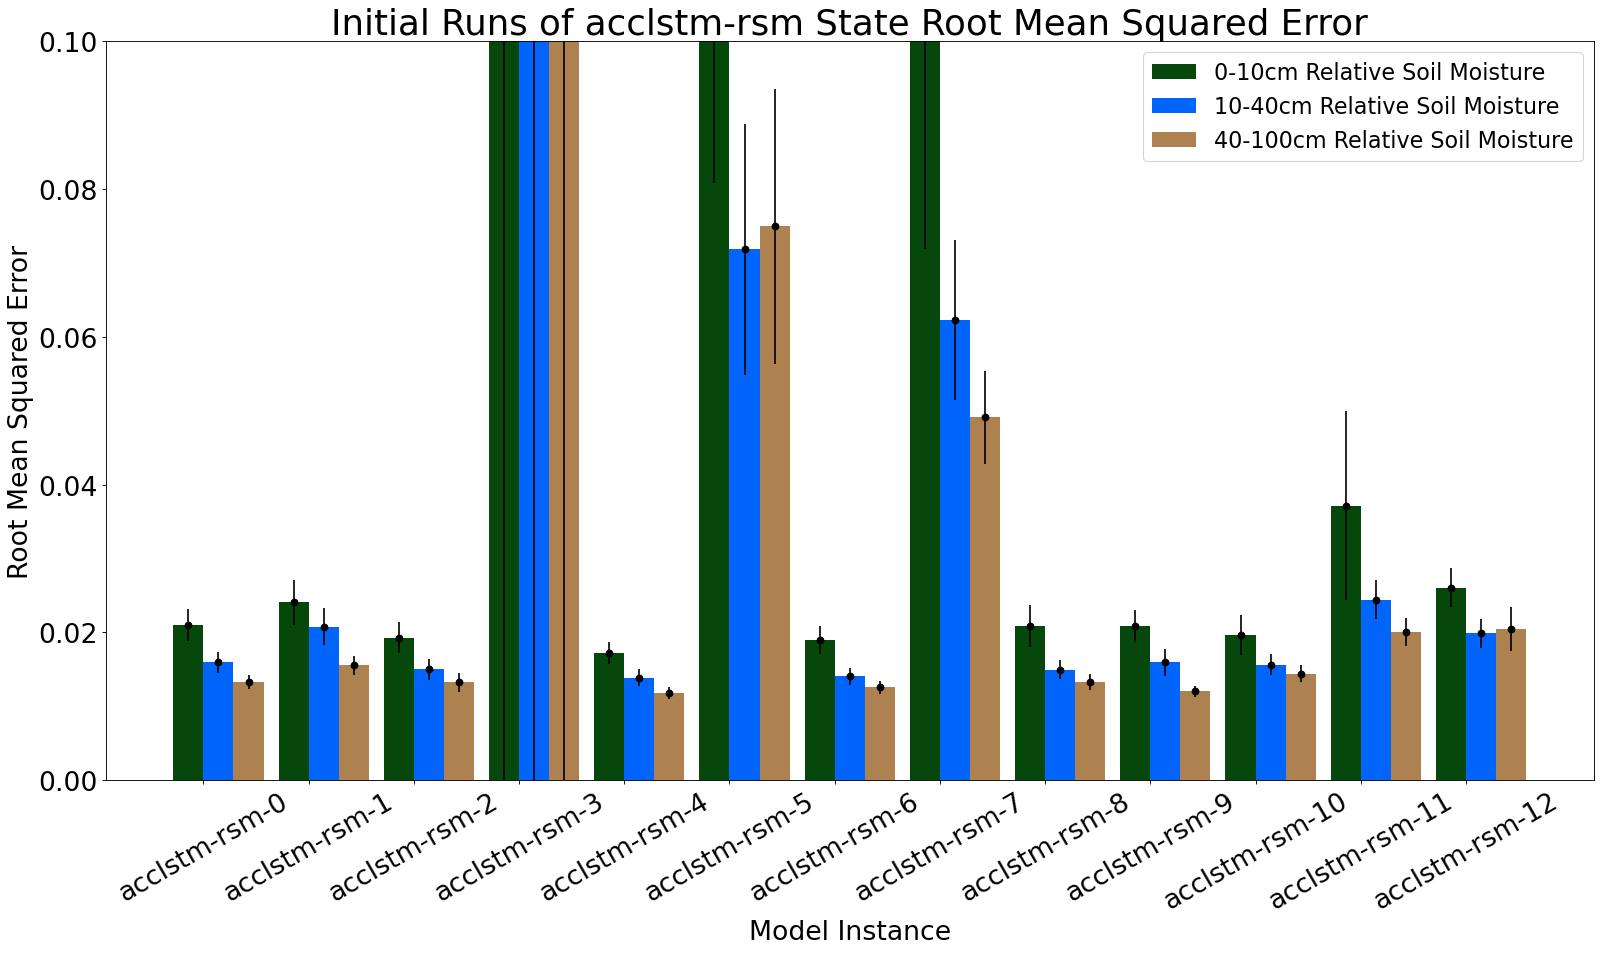
\includegraphics[width=.48\linewidth,draft=false]{figures/efficiency_initial-best/eval_test_efficiency_initial-acclstm-rsm_mse_state.png}
%
%    \caption{Bulk metrics for initial AccLSTM-RSM training runs}
%    \label{model-init-acclstm-rsm}
%\end{figure}
%
%\begin{sidewaystable}
%\begin{center}
%    \begin{tabular}{c|c|c|c|c|c|c }
%    \end{tabular}
%\end{center}
%\end{sidewaystable}


\section{Best Models' Bulk Statistics Comparison}

As Table \ref{model-init-best-table} and Figure \ref{best-metrics} display, the best LSTM-RSM model performed better than the other categories at all of the depth levels, and for each of the evaluation metrics, followed by the LSTM-VSM, and finally the FNN architecture. During evaluation on the full 2018-2023 test dataset, we recorded the execution speed of each of the models as they were applied to multiple subdomains with varying numbers of valid pixels, then fitted a linear regression to the relationship between subdomain size and the time it took to generate a 2-week prediction for each pixel. Evaluation was done with a single CPU thread on a shared high-performance computing cluster. The results in Table \ref{best-exec-efficiency-table} indicate that the initial spin-up time of each model is between 3 and 4 seconds, and execution time for each subsequent pixel is between .1 and 1 millisecond, and is directly proportional to the number of trainable weights in each of the models. When applied to the full domain of 50,875 pixels, the FNN was by far the fastest model at only around 9.5 seconds, while the LSTM variants clocked in at a bit over 40 seconds.

\begin{figure}[hp!]
    \centering
    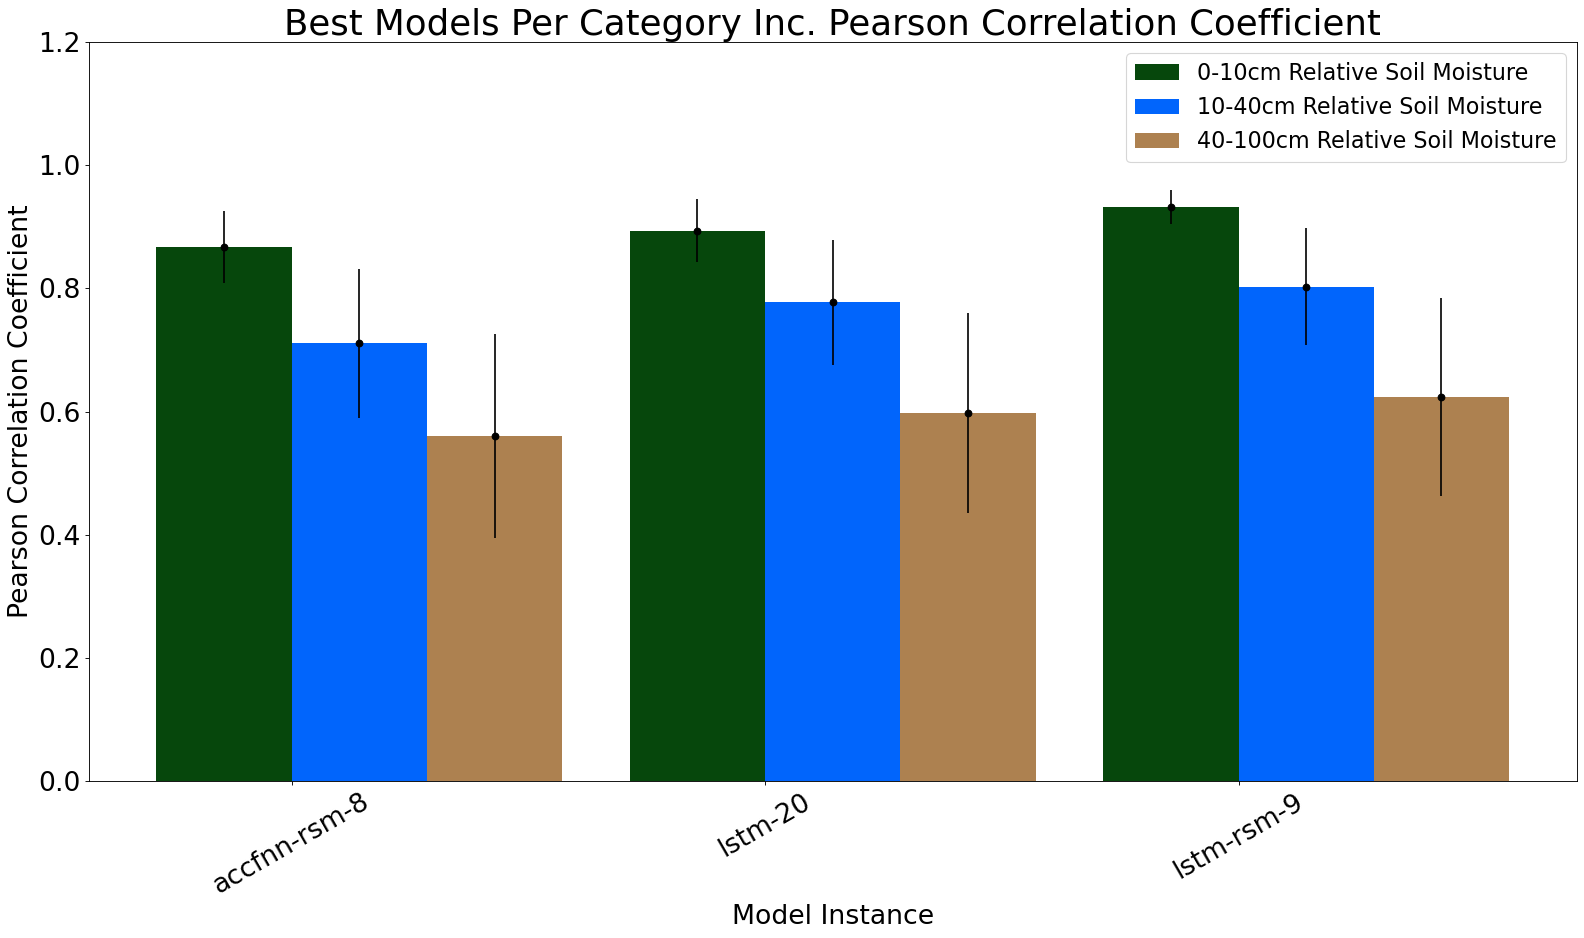
\includegraphics[width=.48\linewidth,draft=false]{figures/efficiency_initial-best/eval_test_efficiency_initial-best_cc_res.png}
    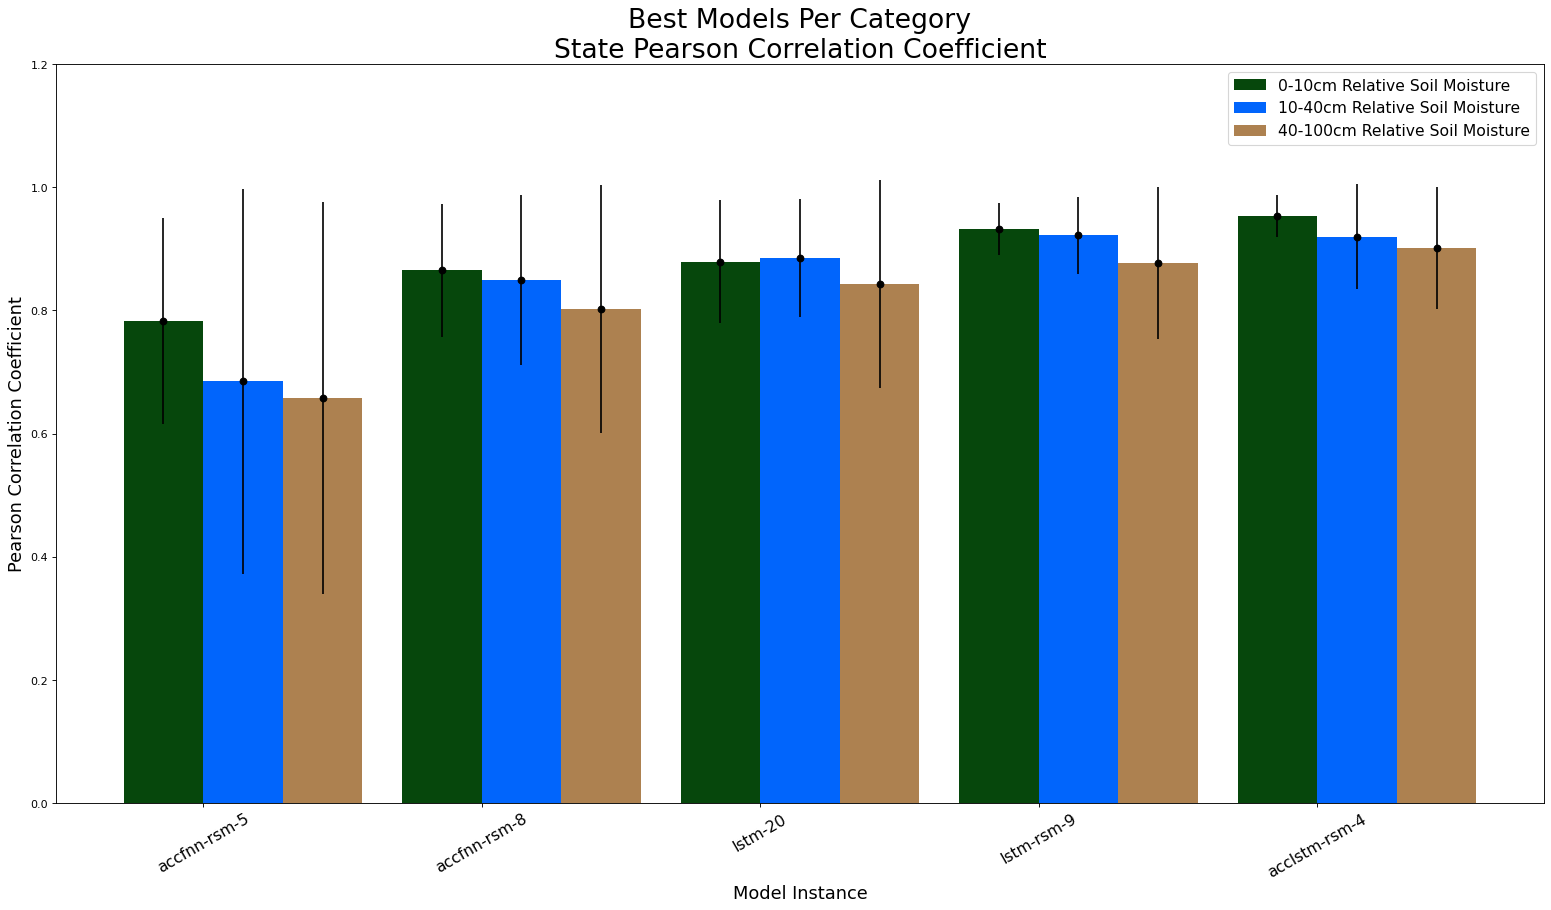
\includegraphics[width=.48\linewidth,draft=false]{figures/efficiency_initial-best/eval_test_efficiency_initial-best_cc_state.png}

    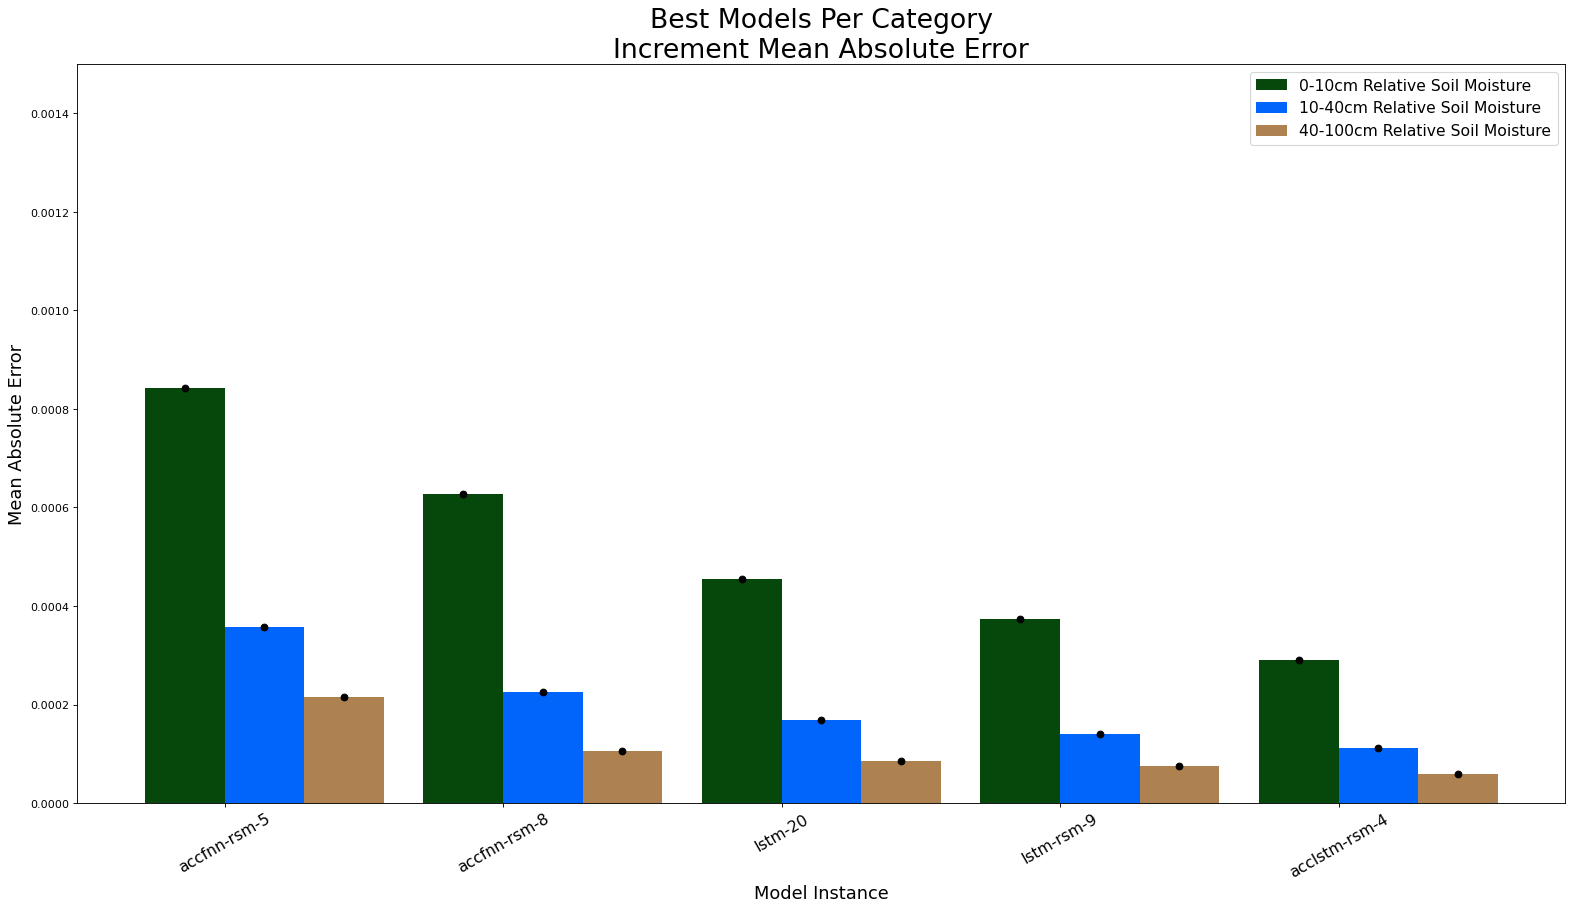
\includegraphics[width=.48\linewidth,draft=false]{figures/efficiency_initial-best/eval_test_efficiency_initial-best_mae_res.png}
    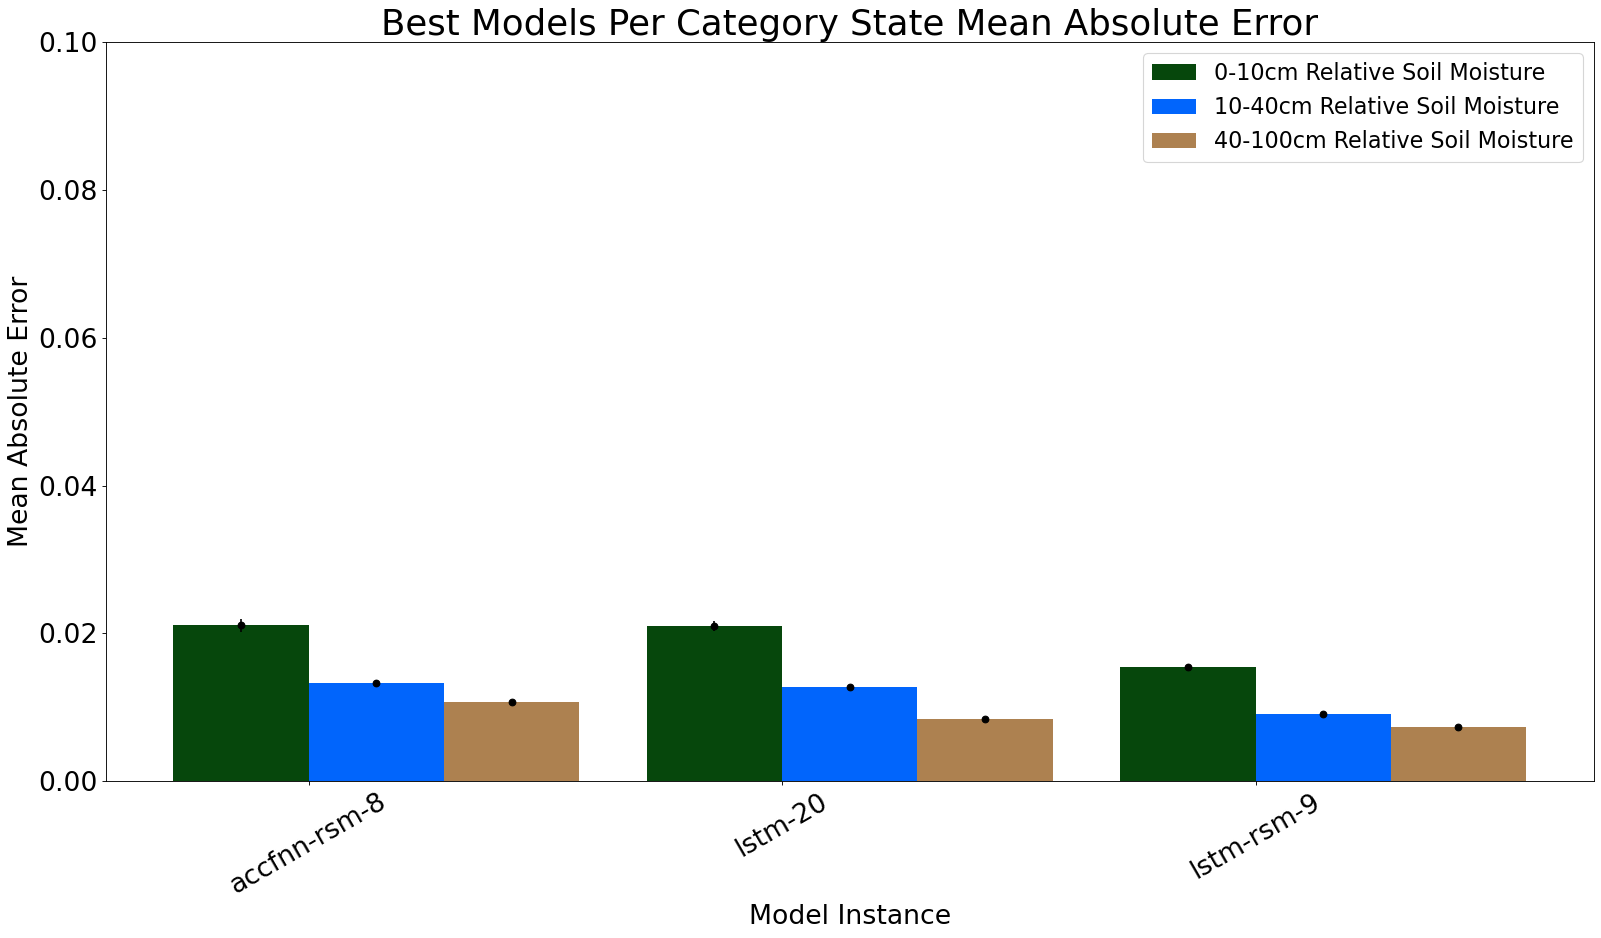
\includegraphics[width=.48\linewidth,draft=false]{figures/efficiency_initial-best/eval_test_efficiency_initial-best_mae_state.png}

    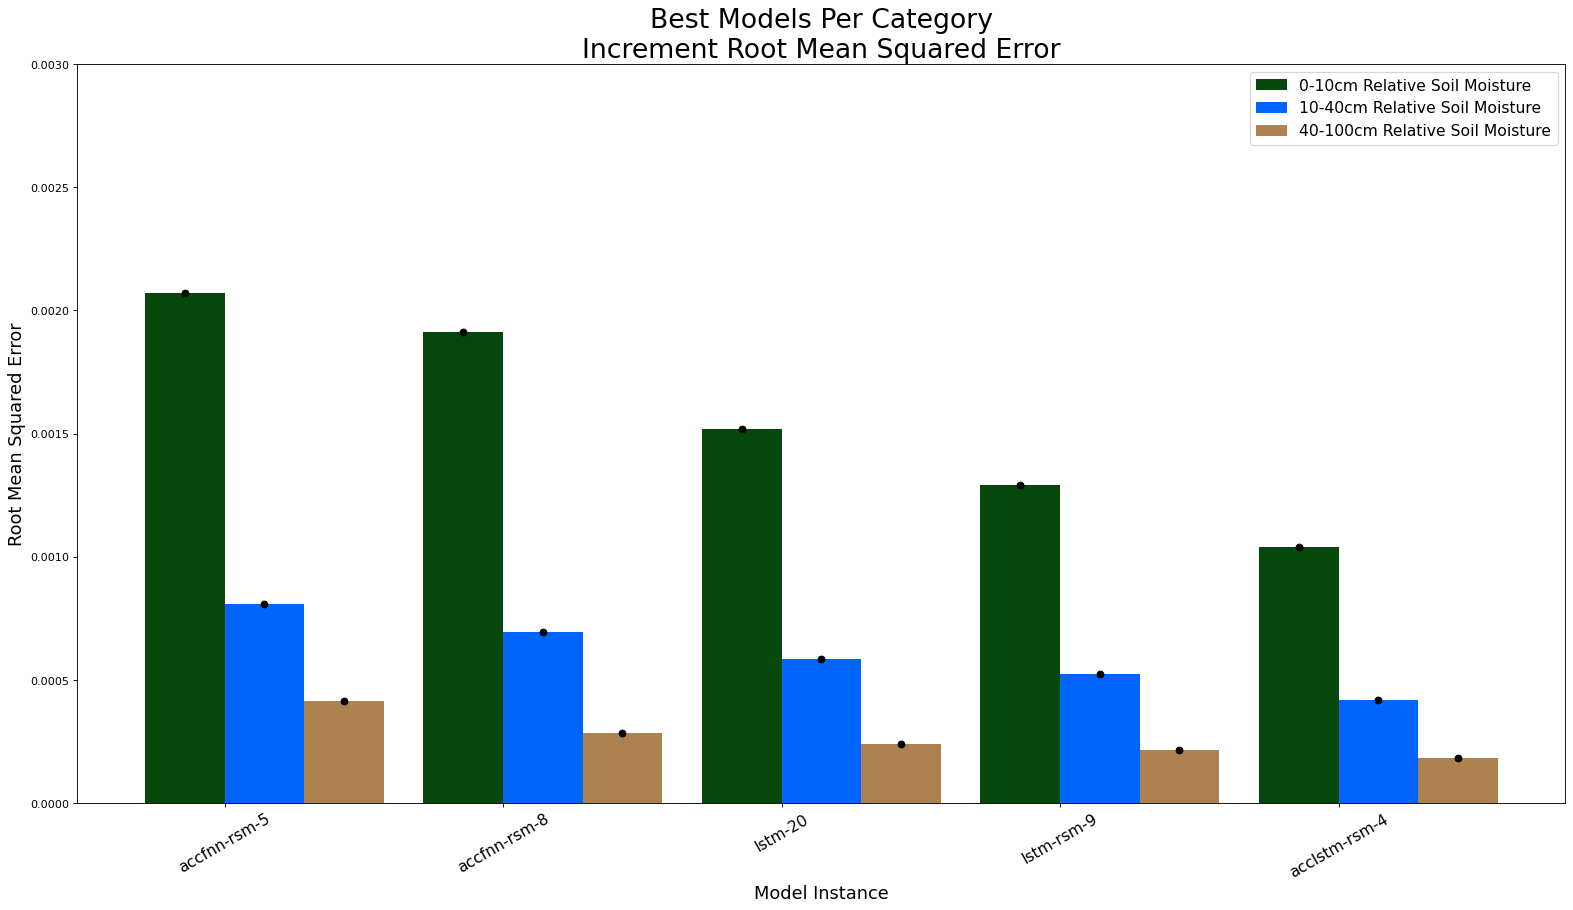
\includegraphics[width=.48\linewidth,draft=false]{figures/efficiency_initial-best/eval_test_efficiency_initial-best_mse_res.png}
    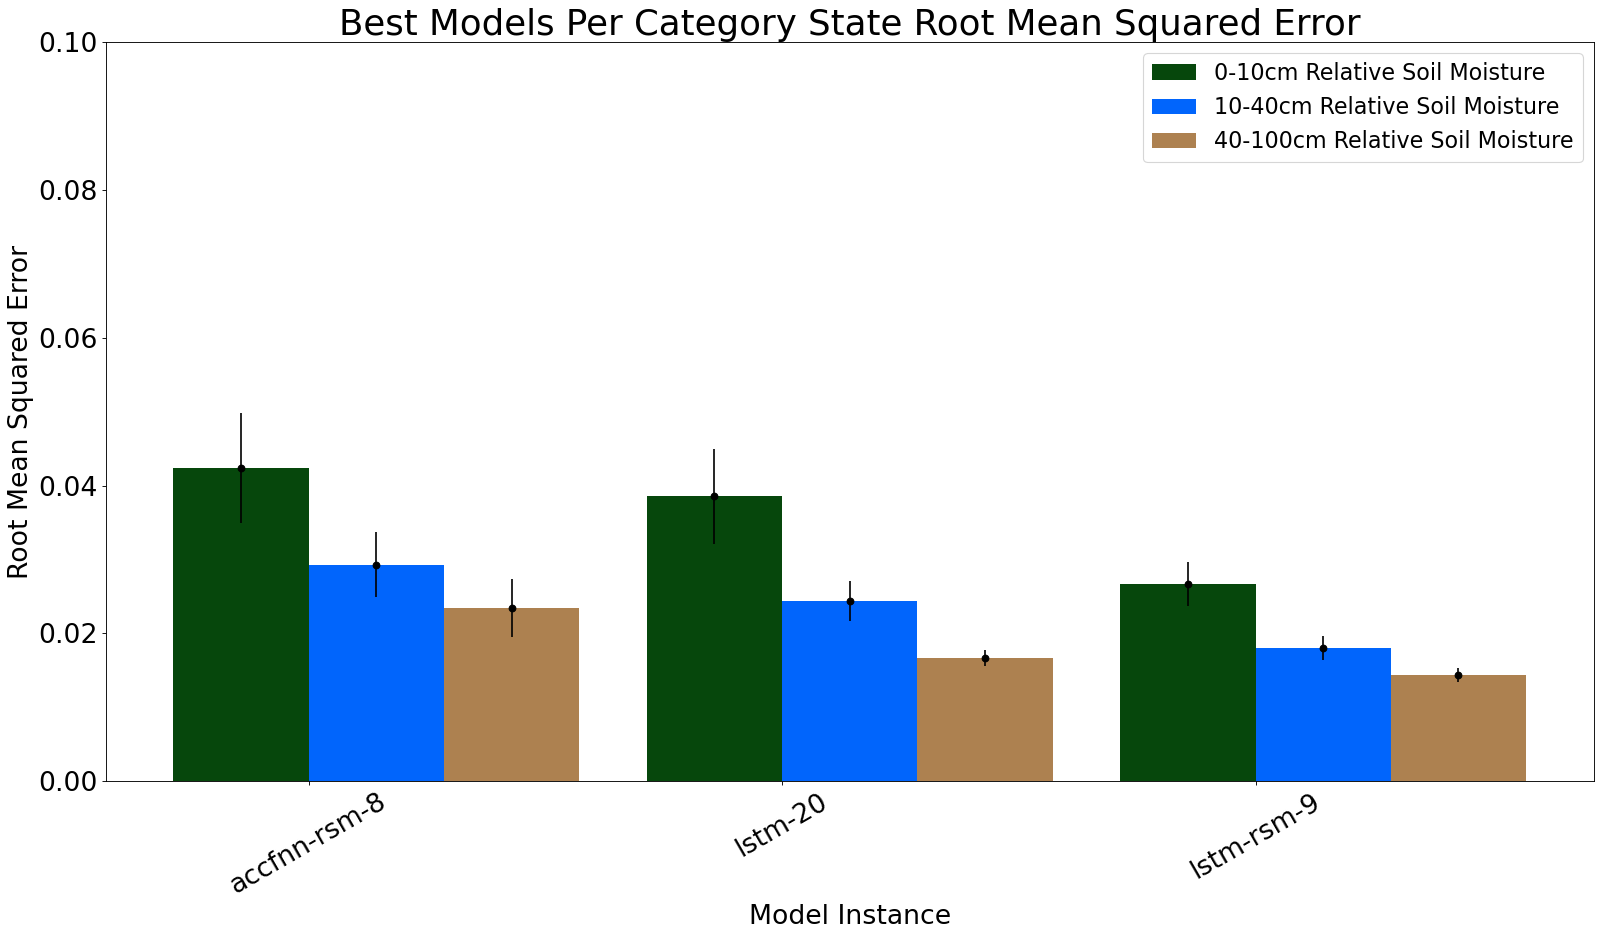
\includegraphics[width=.48\linewidth,draft=false]{figures/efficiency_initial-best/eval_test_efficiency_initial-best_mse_state.png}

    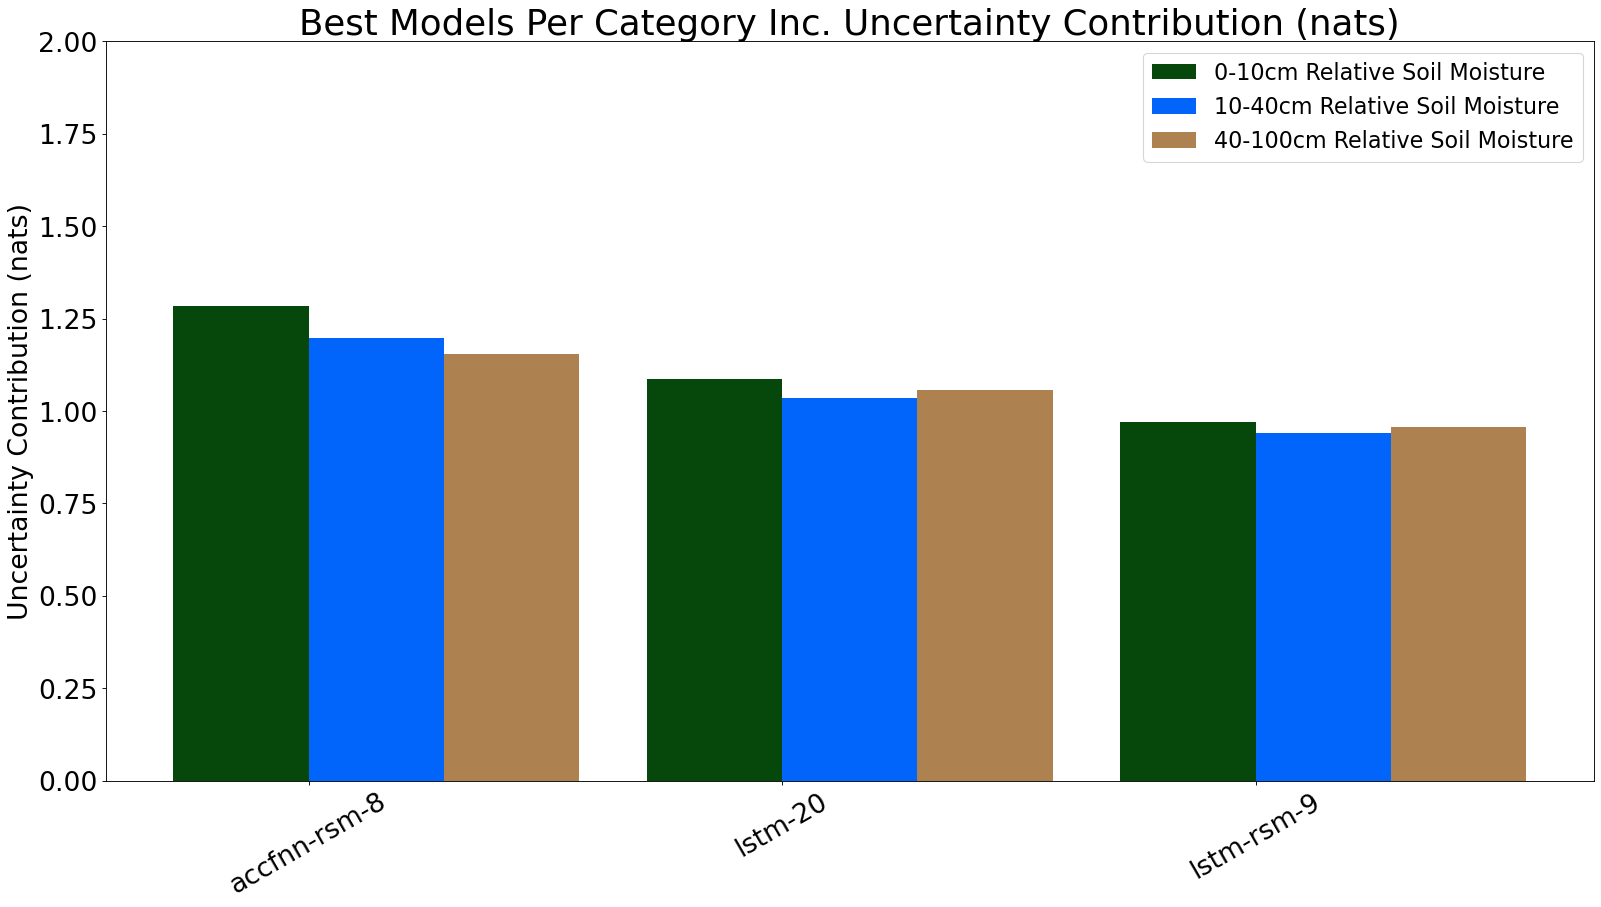
\includegraphics[width=.48\linewidth,draft=false]{figures/efficiency_initial-best/eval_test_efficiency_initial-best_info-loss_res.png}
    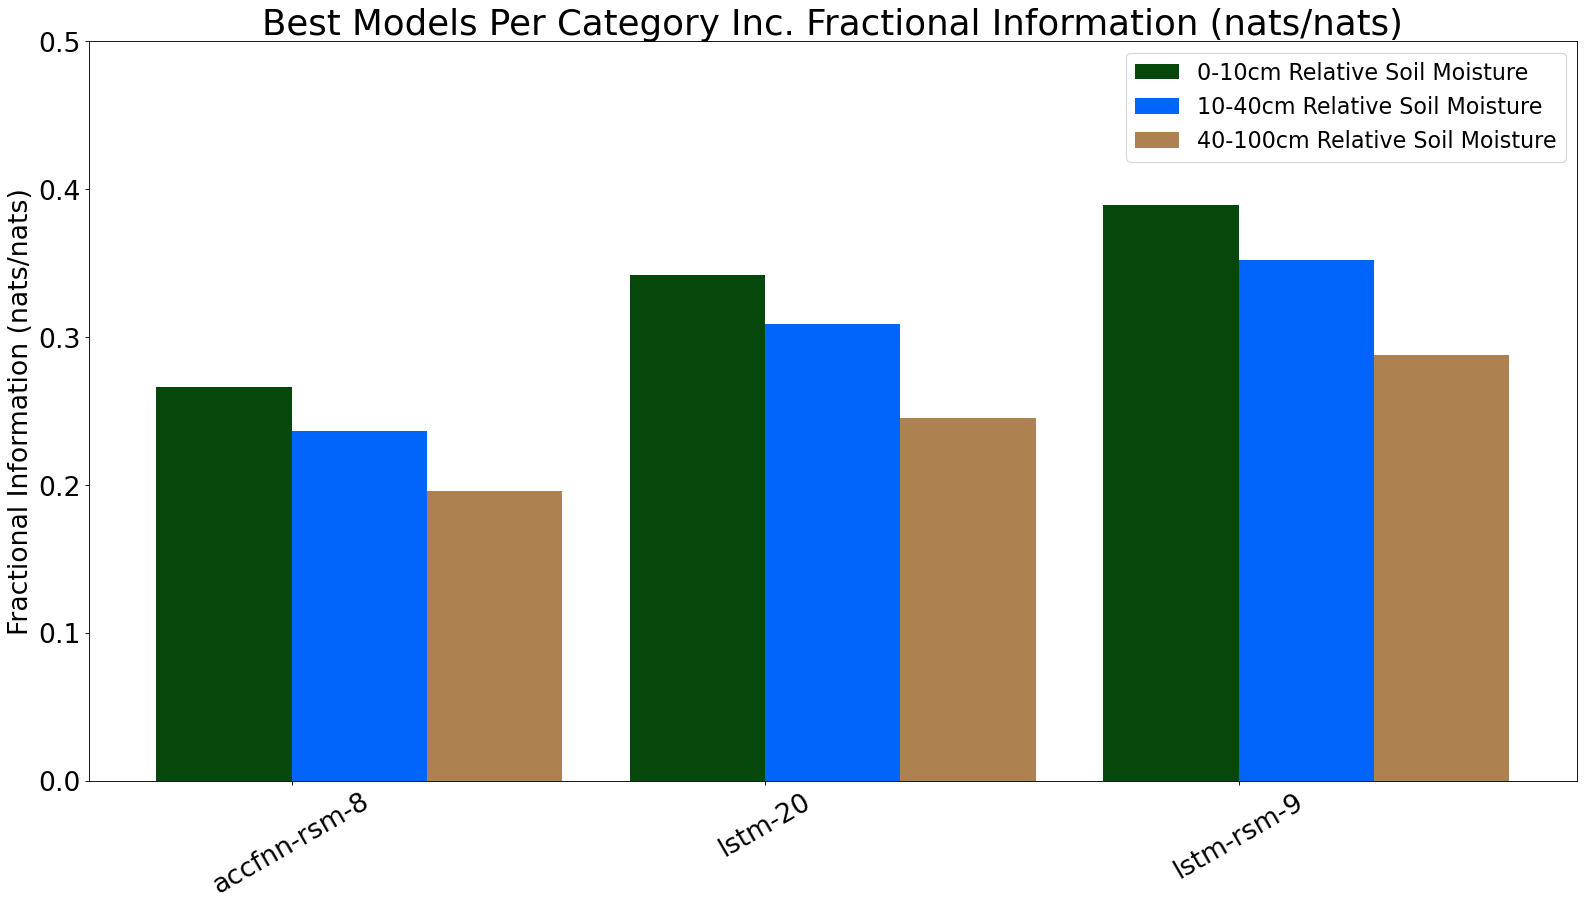
\includegraphics[width=.48\linewidth,draft=false]{figures/efficiency_initial-best/eval_test_efficiency_initial-best_fi_res.png}

    \caption{Bulk metrics comparing the best exploratory models from each category}
    \label{best-metrics}
\end{figure}

\begin{table}[H]
    \centering
    \begin{tabular}{c|c|c|c|c }
        Name & Slope ($ms$) & Intercept ($\frac{s}{px}$) & R$^2$ & Full Domain ($s$) \\
        \hline
        accfnn-rsm-8 & .1262 & 3.088 & .852 & 9.508 \\
        lstm-20 & .8233 & 3.510 & .984 & 45.397 \\
        lstm-rsm-9 & .7544 & 3.246 & .953 & 41.627 \\
    \end{tabular}
    \caption{Linear regression of execution speed for each of the best models.}
    \label{best-exec-efficiency-table}
\end{table}

\begin{table}[H]
    \centering
    \begin{tabular}{c|c|c|c|c|c}
Name &  Weights & \thead{State\\MAE} & \thead{State\\CC} & \thead{Info\\Loss} &\thead{Frac.\\Info}\\
\hline
\multirow{3}{6em}{accfnn-rsm-8} &  \multirow{3}{4em}{30843} & 0.021 & 0.867 & 1.283 & 0.266 \\ & & 0.013 & 0.850 & 1.197 & 0.236 \\ & & 0.011 & 0.809 & 1.154 & 0.196 \\
\hline
\multirow{3}{6em}{lstm-20} &  \multirow{3}{4em}{77117} & 0.021 & 0.882 & 1.088 & 0.342 \\ & & 0.013 & 0.884 & 1.036 & 0.309 \\ & & 0.008 & 0.842 & 1.058 & 0.246 \\
\hline
\multirow{3}{6em}{lstm-rsm-9} & \multirow{3}{4em}{48667} & 0.015 & 0.932 & 0.970 & 0.389 \\ & & 0.009 & 0.922 & 0.941 & 0.352 \\ & & 0.007 & 0.877 & 0.958 & 0.288 \\
    \end{tabular}

    \caption{Size and bulk statistic values of the best models from each category.}
    \label{model-init-best-table}
\end{table}

\begin{figure}[hp!]
    \centering

    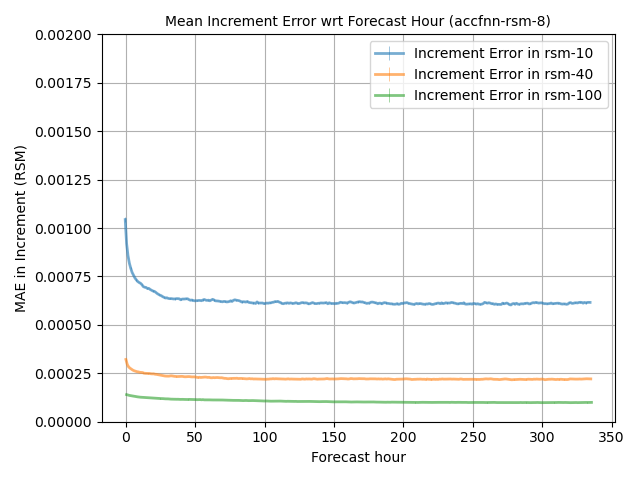
\includegraphics[width=.42\linewidth,draft=false]{figures/horizons/eval_best-redo_accfnn-rsm-8_rsm_horizon_na_res.png}
    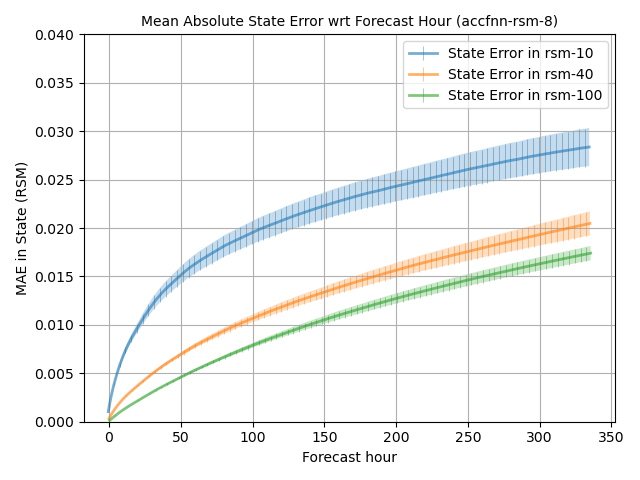
\includegraphics[width=.42\linewidth,draft=false]{figures/horizons/eval_best-redo_accfnn-rsm-8_rsm_horizon_na_state.png}

    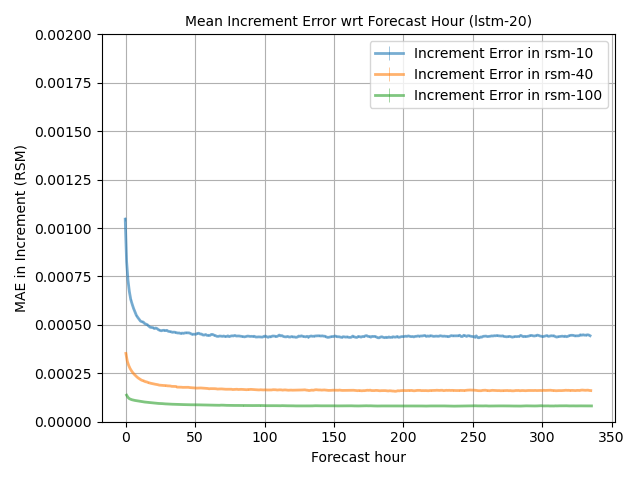
\includegraphics[width=.42\linewidth,draft=false]{figures/horizons/eval_best-redo_lstm-20_rsm_horizon_na_res.png}
    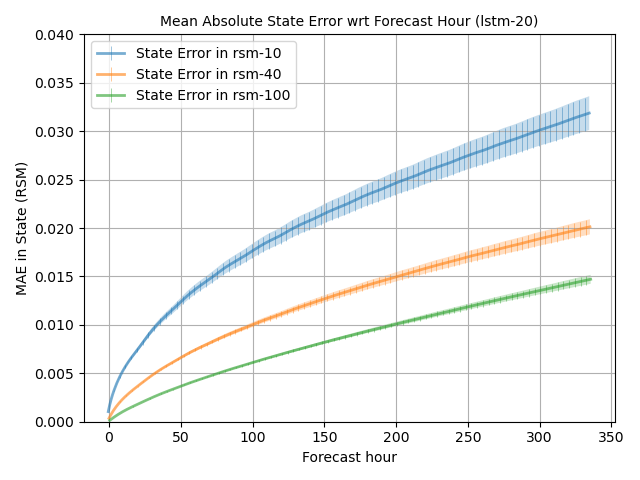
\includegraphics[width=.42\linewidth,draft=false]{figures/horizons/eval_best-redo_lstm-20_rsm_horizon_na_state.png}

    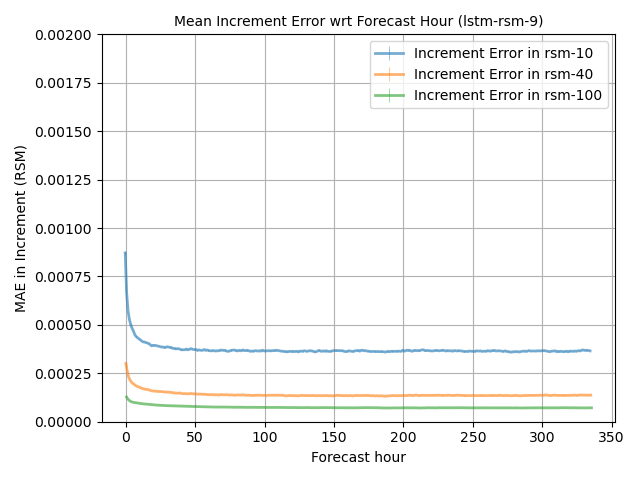
\includegraphics[width=.42\linewidth,draft=false]{figures/horizons/eval_best-redo_lstm-rsm-9_rsm_horizon_na_res.png}
    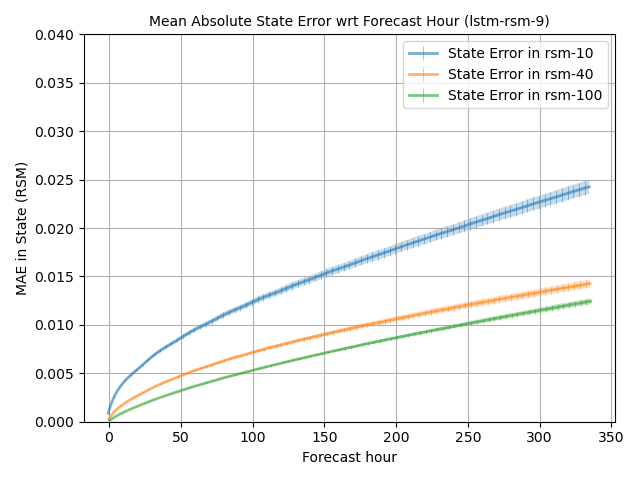
\includegraphics[width=.42\linewidth,draft=false]{figures/horizons/eval_best-redo_lstm-rsm-9_rsm_horizon_na_state.png}

    %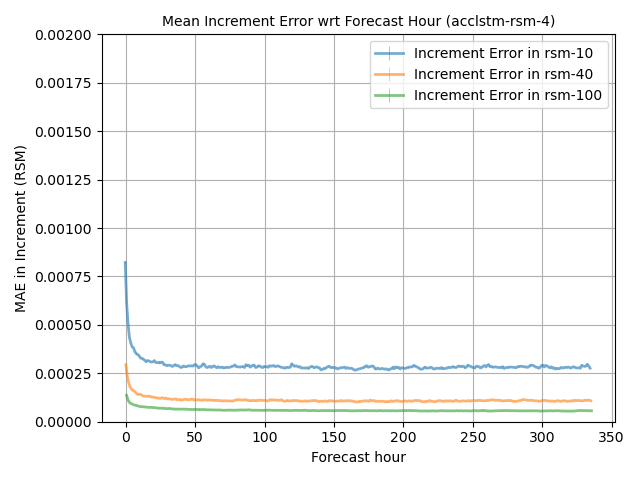
\includegraphics[width=.42\linewidth,draft=false]{figures/horizons/eval_test_acclstm-rsm-4_rsm_horizon_na_res.png}
    %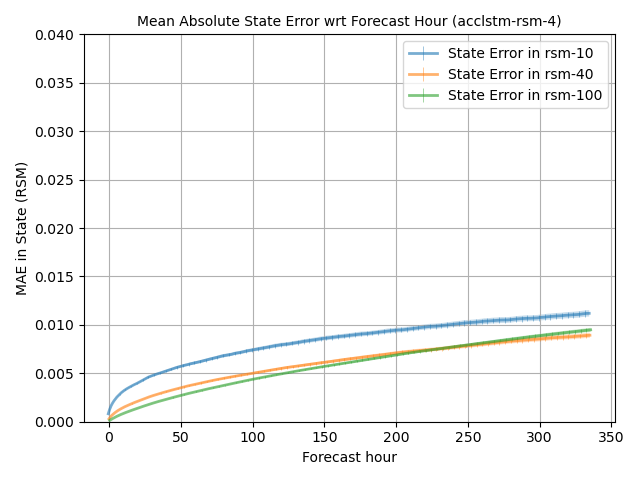
\includegraphics[width=.42\linewidth,draft=false]{figures/horizons/eval_test_acclstm-rsm-4_rsm_horizon_na_state.png}

    \caption{Mean absolute error of each model type with respect to forecast horizon increment (left) and state (right)}
    \label{best-horizons}
\end{figure}

The highest error rates in terms of RSM for each of were associated with the 0-10cm surface layer, which is unsurprising considering that a larger number of processes within Noah-LSM affect the soil dynamics within the topmost layer, which is uniquely influenced by bare-surface evaporation and infiltration from rain and canopy percolation. Furthermore, since the soil layers increase in thickness within Noah-LSM from 10cm at the surface layer to 30cm and 60cm for the deeper layers, each kilogram of actual water mass corresponds to a smaller increment of RSM as it drains downward.

Figure \ref{best-horizons} shows the mean absolute error in RSM for each of the best models with respect to the forecst horizon distance in hours from initialization time. One surprising result that appears universal among the models we trained is that the first few prediction steps consistently have the highest average error in the increment change. For the LSTMs, this could be an indication that the 24 hour spin-up encoder used to initialize the RNN latent vectors prior to the first prediction step have room for improvement, however the FNN has no such encoder. The cause of this spike in error is presently unclear, however in practice, this issue could be mitigated by initializing prediction a few hours prior to the actual initial unknown forecast step, and discarding the first troublesome predictions of increment change.

%\begin{figure}[hp!]
%    \centering
%
%    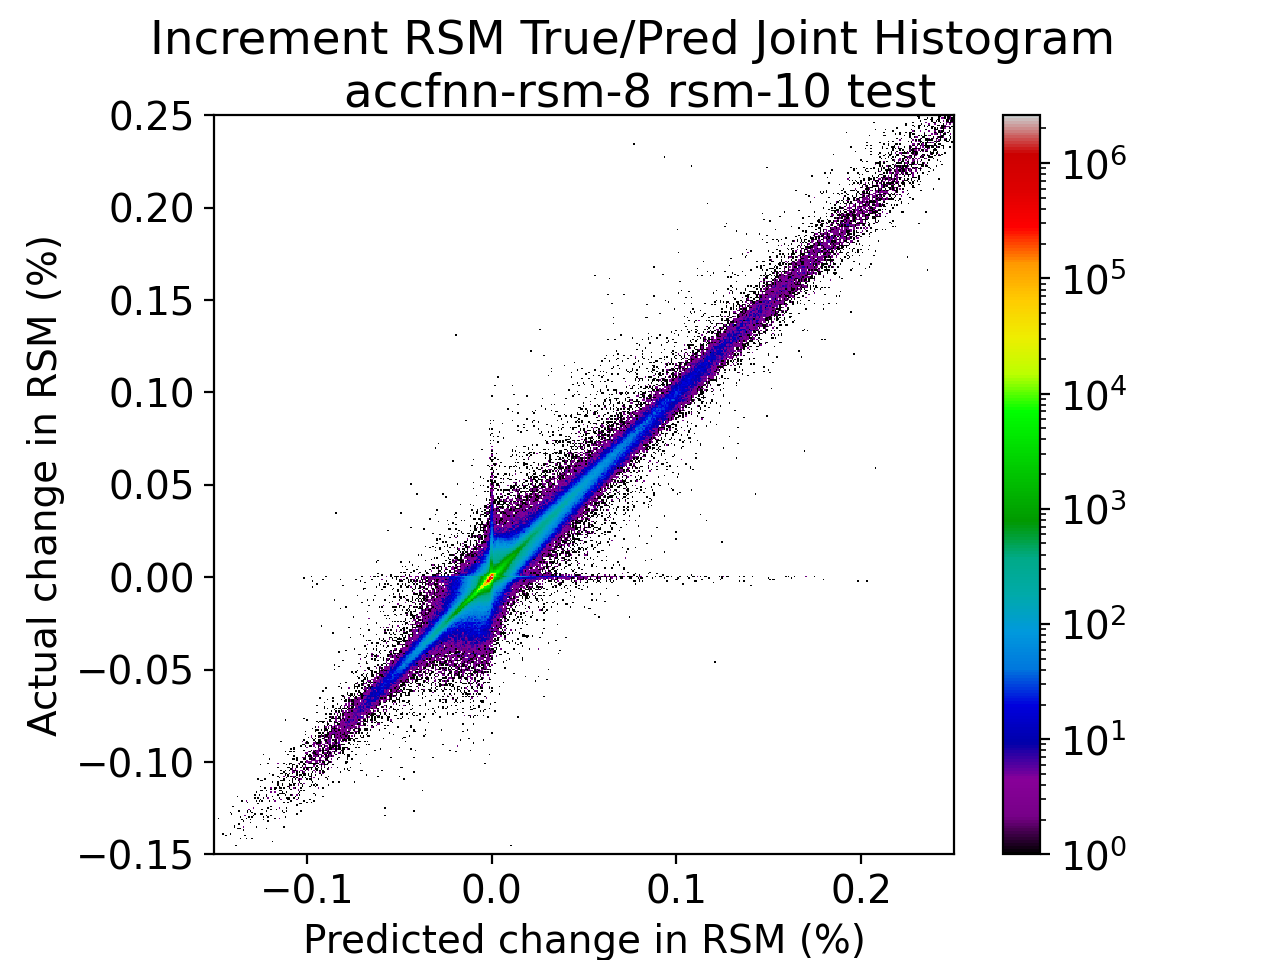
\includegraphics[width=.32\linewidth,draft=false]{figures/validation-curves/eval_test_accfnn-rsm-8_rsm-10_hist-true-pred_na.png}
%    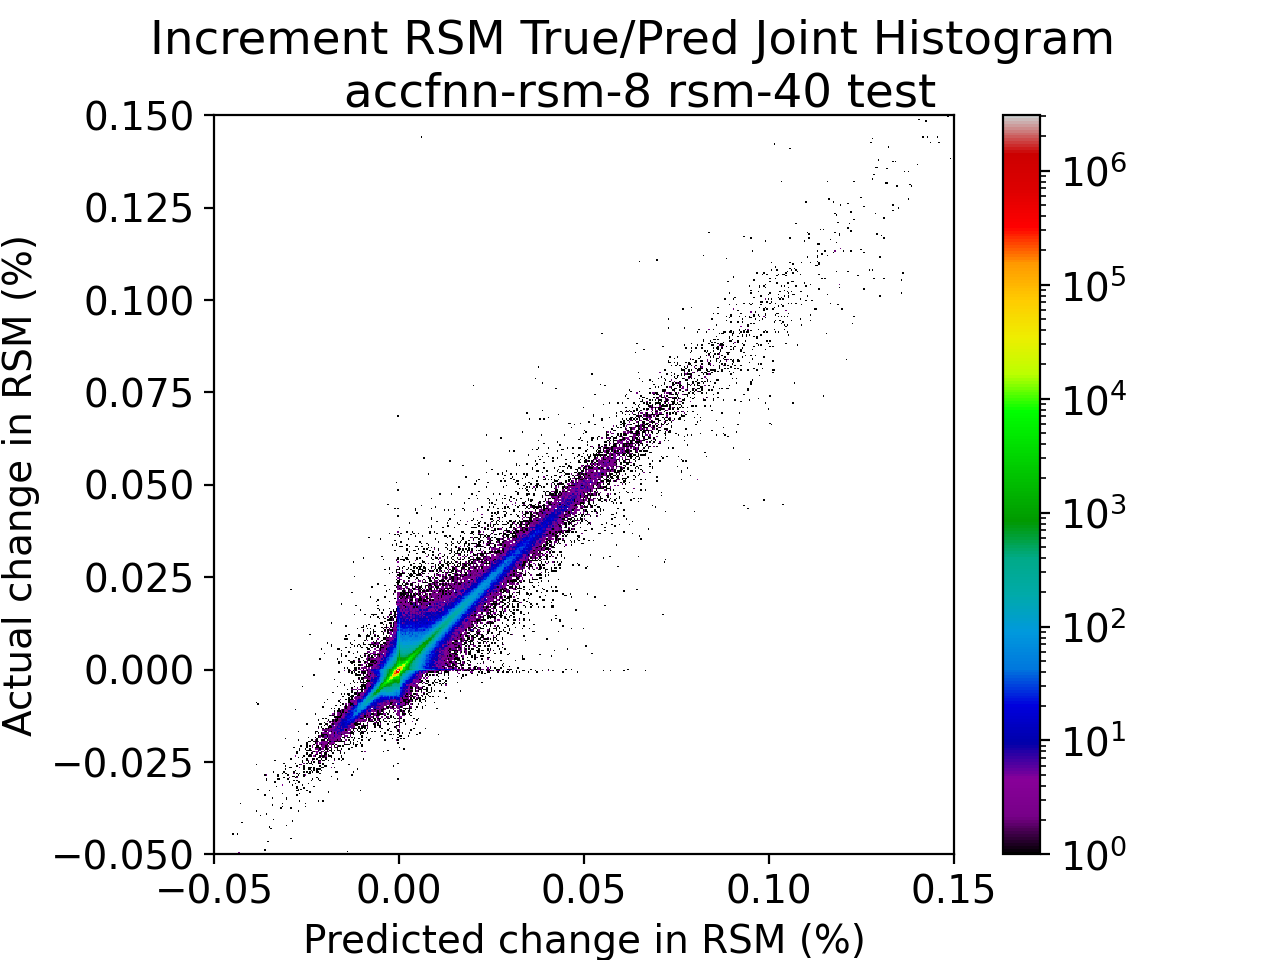
\includegraphics[width=.32\linewidth,draft=false]{figures/validation-curves/eval_test_accfnn-rsm-8_rsm-40_hist-true-pred_na.png}
%    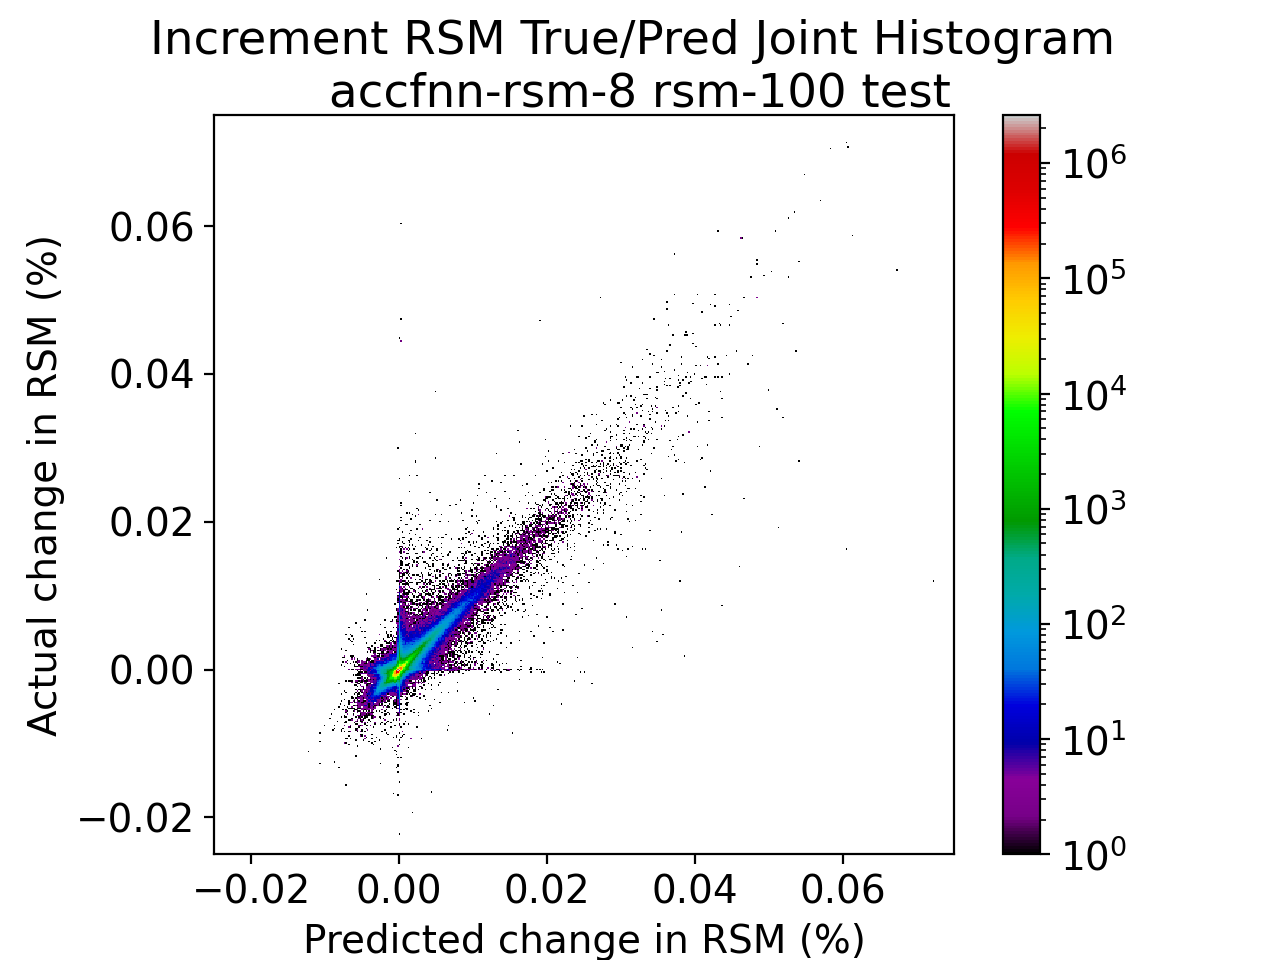
\includegraphics[width=.32\linewidth,draft=false]{figures/validation-curves/eval_test_accfnn-rsm-8_rsm-100_hist-true-pred_na.png}
%
%    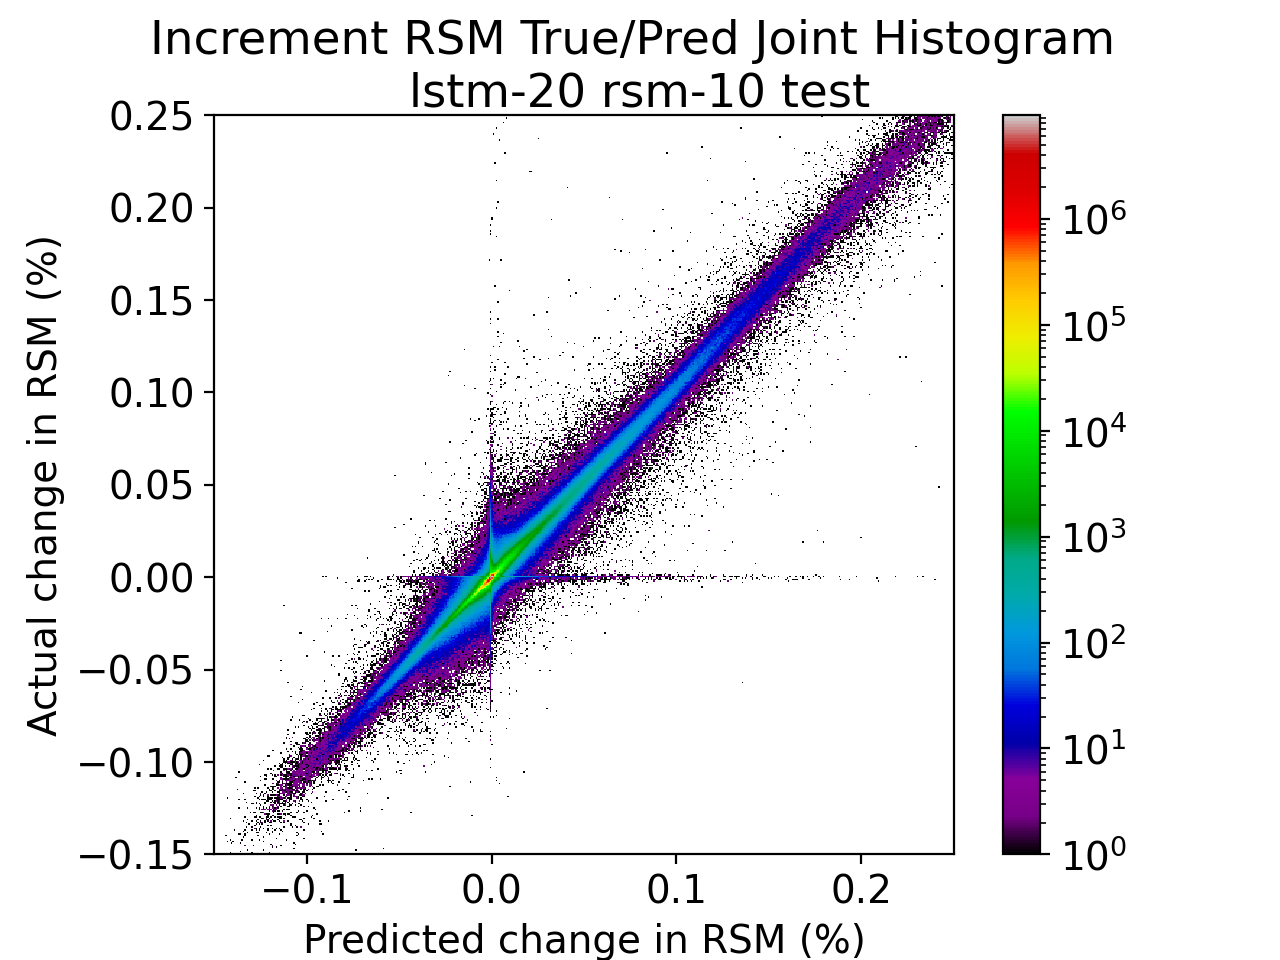
\includegraphics[width=.32\linewidth,draft=false]{figures/validation-curves/eval_test_lstm-20_rsm-10_hist-true-pred_na.png}
%    \includegraphics[width=.32\linewidth,draft=false]{figures/validation-curves/eval_test_lstm-20_rsm-40_hist-true-pred_na.png}
%    \includegraphics[width=.32\linewidth,draft=false]{figures/validation-curves/eval_test_lstm-20_rsm-100_hist-true-pred_na.png}
%
%    \includegraphics[width=.32\linewidth,draft=false]{figures/validation-curves/eval_test_lstm-rsm-9_rsm-10_hist-true-pred_na.png}
%    \includegraphics[width=.32\linewidth,draft=false]{figures/validation-curves/eval_test_lstm-rsm-9_rsm-40_hist-true-pred_na.png}
%    \includegraphics[width=.32\linewidth,draft=false]{figures/validation-curves/eval_test_lstm-rsm-9_rsm-100_hist-true-pred_na.png}
%
%    %\includegraphics[width=.32\linewidth,draft=false]{figures/validation-curves/eval_test_acclstm-rsm-4_rsm-10_hist-true-pred_na.png}
%    %\includegraphics[width=.32\linewidth,draft=false]{figures/validation-curves/eval_test_acclstm-rsm-4_rsm-40_hist-true-pred_na.png}
%    %\includegraphics[width=.32\linewidth,draft=false]{figures/validation-curves/eval_test_acclstm-rsm-4_rsm-100_hist-true-pred_na.png}
%
%    \caption{Heatmaps of true/predicted joint histograms for each of the top 3 soil layers, as predicted by the best models from each category.}
%    \label{best-validation}
%\end{figure}

%\begin{figure}[hp!]
%    \centering
%
%    \includegraphics[width=.32\linewidth,draft=false]{figures/static-combos/eval_test_accfnn-rsm-8_rsm-10_static-combos_abs-err_state.png}
%    \includegraphics[width=.32\linewidth,draft=false]{figures/static-combos/eval_test_accfnn-rsm-8_rsm-40_static-combos_abs-err_state.png}
%    \includegraphics[width=.32\linewidth,draft=false]{figures/static-combos/eval_test_accfnn-rsm-8_rsm-100_static-combos_abs-err_state.png}
%
%    \includegraphics[width=.32\linewidth,draft=false]{figures/static-combos/eval_test_lstm-20_rsm-10_static-combos_abs-err_state.png}
%    \includegraphics[width=.32\linewidth,draft=false]{figures/static-combos/eval_test_lstm-20_rsm-40_static-combos_abs-err_state.png}
%    \includegraphics[width=.32\linewidth,draft=false]{figures/static-combos/eval_test_lstm-20_rsm-100_static-combos_abs-err_state.png}
%
%    \includegraphics[width=.32\linewidth,draft=false]{figures/static-combos/eval_test_lstm-rsm-9_rsm-10_static-combos_abs-err_state.png}
%    \includegraphics[width=.32\linewidth,draft=false]{figures/static-combos/eval_test_lstm-rsm-9_rsm-40_static-combos_abs-err_state.png}
%    \includegraphics[width=.32\linewidth,draft=false]{figures/static-combos/eval_test_lstm-rsm-9_rsm-100_static-combos_abs-err_state.png}
%
%    %\includegraphics[width=.32\linewidth,draft=false]{figures/static-combos/eval_test_acclstm-rsm-4_rsm-10_static-combos_abs-err_state.png}
%    %\includegraphics[width=.32\linewidth,draft=false]{figures/static-combos/eval_test_acclstm-rsm-4_rsm-40_static-combos_abs-err_state.png}
%    %\includegraphics[width=.32\linewidth,draft=false]{figures/static-combos/eval_test_acclstm-rsm-4_rsm-100_static-combos_abs-err_state.png}
%
%    \caption{Absolute error of best models' state from each category with respect to static categorical parameter combinations.}
%    \label{best-static-abserr}
%\end{figure}

%\begin{figure}[hp!]
%    \centering
%
%    \includegraphics[width=.32\linewidth,draft=false]{figures/static-combos/eval_test_accfnn-rsm-8_rsm-10_static-combos_bias_state.png}
%    \includegraphics[width=.32\linewidth,draft=false]{figures/static-combos/eval_test_accfnn-rsm-8_rsm-40_static-combos_bias_state.png}
%    \includegraphics[width=.32\linewidth,draft=false]{figures/static-combos/eval_test_accfnn-rsm-8_rsm-100_static-combos_bias_state.png}
%
%    \includegraphics[width=.32\linewidth,draft=false]{figures/static-combos/eval_test_lstm-20_rsm-10_static-combos_bias_state.png}
%    \includegraphics[width=.32\linewidth,draft=false]{figures/static-combos/eval_test_lstm-20_rsm-40_static-combos_bias_state.png}
%    \includegraphics[width=.32\linewidth,draft=false]{figures/static-combos/eval_test_lstm-20_rsm-100_static-combos_bias_state.png}
%
%    \includegraphics[width=.32\linewidth,draft=false]{figures/static-combos/eval_test_lstm-rsm-9_rsm-10_static-combos_bias_state.png}
%    \includegraphics[width=.32\linewidth,draft=false]{figures/static-combos/eval_test_lstm-rsm-9_rsm-40_static-combos_bias_state.png}
%    \includegraphics[width=.32\linewidth,draft=false]{figures/static-combos/eval_test_lstm-rsm-9_rsm-100_static-combos_bias_state.png}
%
%    %\includegraphics[width=.32\linewidth,draft=false]{figures/static-combos/eval_test_acclstm-rsm-4_rsm-10_static-combos_bias_state.png}
%    %\includegraphics[width=.32\linewidth,draft=false]{figures/static-combos/eval_test_acclstm-rsm-4_rsm-40_static-combos_bias_state.png}
%    %\includegraphics[width=.32\linewidth,draft=false]{figures/static-combos/eval_test_acclstm-rsm-4_rsm-100_static-combos_bias_state.png}
%
%    \caption{Bias of best models' state from each category with respect to static categorical parameter combinations.}
%    \label{best-static-bias}
%\end{figure}

\begin{figure}[hp!]
    \centering

    \includegraphics[width=.48\linewidth,draft=false]{figures/grid-eval_best_full/eval-grid_full_accfnn-rsm-8_rsm-10_spatial-stats_abs-err_state-err-abs-mean.png}
    \includegraphics[width=.48\linewidth,draft=false]{figures/grid-eval_best_full/eval-grid_full_accfnn-rsm-8_rsm-10_spatial-stats_bias_state-err-bias-mean.png}

    \includegraphics[width=.48\linewidth,draft=false]{figures/grid-eval_best_full/eval-grid_full_lstm-20_rsm-10_spatial-stats_abs-err_state-err-abs-mean.png}
    \includegraphics[width=.48\linewidth,draft=false]{figures/grid-eval_best_full/eval-grid_full_lstm-20_rsm-10_spatial-stats_bias_state-err-bias-mean.png}

    \includegraphics[width=.48\linewidth,draft=false]{figures/grid-eval_best_full/eval-grid_full_lstm-rsm-9_rsm-10_spatial-stats_abs-err_state-err-abs-mean.png}
    \includegraphics[width=.48\linewidth,draft=false]{figures/grid-eval_best_full/eval-grid_full_lstm-rsm-9_rsm-10_spatial-stats_bias_state-err-bias-mean.png}

    \caption{Gridded MAE and bias in state for each of the best models at the 0-10cm depth level, evaluated on full test set (2018-2023)}
    \label{grid-full_rsm-10}
\end{figure}

\begin{figure}[hp!]
    \centering

    \includegraphics[width=.48\linewidth,draft=false]{figures/grid-eval_best_full/eval-grid_full_accfnn-rsm-8_rsm-40_spatial-stats_abs-err_state-err-abs-mean.png}
    \includegraphics[width=.48\linewidth,draft=false]{figures/grid-eval_best_full/eval-grid_full_accfnn-rsm-8_rsm-40_spatial-stats_bias_state-err-bias-mean.png}

    \includegraphics[width=.48\linewidth,draft=false]{figures/grid-eval_best_full/eval-grid_full_lstm-20_rsm-40_spatial-stats_abs-err_state-err-abs-mean.png}
    \includegraphics[width=.48\linewidth,draft=false]{figures/grid-eval_best_full/eval-grid_full_lstm-20_rsm-40_spatial-stats_bias_state-err-bias-mean.png}

    \includegraphics[width=.48\linewidth,draft=false]{figures/grid-eval_best_full/eval-grid_full_lstm-rsm-9_rsm-40_spatial-stats_abs-err_state-err-abs-mean.png}
    \includegraphics[width=.48\linewidth,draft=false]{figures/grid-eval_best_full/eval-grid_full_lstm-rsm-9_rsm-40_spatial-stats_bias_state-err-bias-mean.png}

    \caption{Gridded MAE and bias in state for each of the best models at the 10-40cm depth level, evaluated on full test set (2018-2023)}
    \label{grid-full_rsm-40}
\end{figure}

\begin{figure}[hp!]
    \centering

    \includegraphics[width=.48\linewidth,draft=false]{figures/grid-eval_best_full/eval-grid_full_accfnn-rsm-8_rsm-100_spatial-stats_abs-err_state-err-abs-mean.png}
    \includegraphics[width=.48\linewidth,draft=false]{figures/grid-eval_best_full/eval-grid_full_accfnn-rsm-8_rsm-100_spatial-stats_bias_state-err-bias-mean.png}

    \includegraphics[width=.48\linewidth,draft=false]{figures/grid-eval_best_full/eval-grid_full_lstm-20_rsm-100_spatial-stats_abs-err_state-err-abs-mean.png}
    \includegraphics[width=.48\linewidth,draft=false]{figures/grid-eval_best_full/eval-grid_full_lstm-20_rsm-100_spatial-stats_bias_state-err-bias-mean.png}

    \includegraphics[width=.48\linewidth,draft=false]{figures/grid-eval_best_full/eval-grid_full_lstm-rsm-9_rsm-100_spatial-stats_abs-err_state-err-abs-mean.png}
    \includegraphics[width=.48\linewidth,draft=false]{figures/grid-eval_best_full/eval-grid_full_lstm-rsm-9_rsm-100_spatial-stats_bias_state-err-bias-mean.png}

    \caption{Gridded MAE and bias in state for each of the best models at the 40-100cm depth level, evaluated on full test set (2018-2023)}
    \label{grid-full_rsm-100}
\end{figure}

Figures \ref{grid-full_rsm-10}, \ref{grid-full_rsm-40}, and \ref{grid-full_rsm-100} show the overall spatial distribution of mean absolute error and model bias at the 0-10cm, 10-40cm, and 40-100cm depth levels, respectively. We will use the information that these graphics provide to identify areas of anomalous model behavior for further investigation in the following section.

The LSTM-RSM shows a widespread slight dry bias in the surface layer with the exception of urban areas, mountainous regions, and some sandy areas in Texas, New Mexico, and the Northern Midwest. The LSTM-VSM (lstm-20) largely follows suit, though it also showed regions of wet bias where the LSTM-RSM was more neutral or dry including silty regions corresponding to the Ouachita mountains, central Kentucky and the Cumberland plateu, the Northern Rockies in Idaho and Montana, and Florida. The FNN model had significantly more of a wet bias in the surface layer for some regions, which were largely distinguished discretely by their soil texture boundaries.

All three models had more of a mixture of wet and dry biases in the 10-40cm layer. In the Midwest, Northern Wisconson and Minnesota were dry except for isolated sandy pixels, while the cropland in the Ohio and Missouri River basins to the South and West of that region were notably too wet: a pattern that was further emphasized in the 40-100cm layer. The wet bias associated with the cropland surface type was also apparent in Mississippi Alluvial Plains of Eastern Arkansas and the Missouri Bootheel, discrete regions of East Texas, the Florida Penninsula, and East-central South Carolina. Furthermore, each of the models also demonstrated a wet bias associated with clay-dominant pixels in the Centeral Texas and surrounding the Southern extent of the Mississippi River. In addition to the Northeast and Northern Midwest, the regions with the most significant dry bias in the lower two layers seemed to be associated with higher elevation, especially the Sierra Nevada mountains, Colorado Rockies, and Central Idaho, although the Cascades seem to be an exception with a stark wet bias for the LSTM-RSM model.

\begin{figure}[h!]
    \centering
    \includegraphics[width=.66\linewidth,draft=false]{figures/static_slopetype_3km.png}
    \caption{SLOPETYPE classes defining bottom-layer drainage.}
    \label{slopetype-classes}
\end{figure}

In the lower two layers, there is also an anomalous tiling artifact present in the model biases that is especially noticable in the Ohio river valley, Montana, and the central Great Plains. The emerging squares are 8 pixels in length and width, forming a $1^\circ$ grid. This was initially perplexing since no similar pattern appears in the forcings, however close inspection of the mean Noah-LSM soil moisture content in 40-100cm layer of Figure \ref{gs-rsm} also reveals subtle edges that correspond to the bias tiles. Upon further investigation, we found that the square boundaries closely align with an input parameter in Noah-LSM called SLOPETYPE which controls the rate at which water drains out of the lowest layer of the model by applying one of 9 discrete classes \citep{mitchell_community_2005}, which are displayed by Figure \ref{slopetype-classes}. This parameter is distinct from the surface slope (which is defined in terms of degrees from vertical), and wasn't provided as an input to the ANNs during training, so the patterns in model bias are emergent from the unexplained variance introduced by leaving out these values.

Despite the inconsistencies between the models' biases, several regions stand out as especially troublesome in terms of all of the models' mean absolute error. Sandy areas in the Midwest, Nebraska, Oregon, and the Four Corners region of the Desert Southwest have high error rates in the first two layers. In the 40-100cm layer, clay pixels in Mississippi, Louisiana, Alabama, and Northern Ohio suffer, and the Sierra Nevada and Cascade mountains proved especially difficult for the models to characterize in the lower two soil layers.

%\begin{figure}[hp!]
%    \centering
%
%    \includegraphics[width=.96\linewidth,draft=false]{figures/grid-eval_best_full/eval-grid_full_lstm-rsm-9_rsm-10_hist-humidity-temp_abs-err.png}
%    \includegraphics[width=.96\linewidth,draft=false]{figures/grid-eval_best_full/eval-grid_full_lstm-rsm-9_rsm-10_hist-humidity-temp_bias.png}
%
%    \caption{Joint histogram of humidity and temperature forcings, with mean absolute error (top) and error bias (bottom) plotted within corresponding bins.}
%    \label{lstm-rsm-9-hthist}
%\end{figure}

%\begin{figure}[hp!]
%    \centering
%
%    \includegraphics[width=.96\linewidth,draft=false]{figures/grid-eval_best_full/eval-grid_full_lstm-rsm-9_rsm-10_hist-state-increment_abs-err.png}
%    \includegraphics[width=.96\linewidth,draft=false]{figures/grid-eval_best_full/eval-grid_full_lstm-rsm-9_rsm-10_hist-state-increment_bias.png}
%
%    \caption{Joint histogram of total RSM and increment change of RSM in the 0-10cm layer, with mean absolute error (top) and error bias (bottom) plotted within corresponding bins.}
%    \label{lstm-rsm-9-sihist-rsm-10}
%\end{figure}

%\begin{figure}[hp!]
%    \centering
%
%    \includegraphics[width=.96\linewidth,draft=false]{figures/grid-eval_lstm-rsm-9_full/eval-grid_full_lstm-rsm-9_rsm-40_hist-state-increment_abs-err.png}
%    \includegraphics[width=.96\linewidth,draft=false]{figures/grid-eval_lstm-rsm-9_full/eval-grid_full_lstm-rsm-9_rsm-40_hist-state-increment_bias.png}
%
%    \caption{Joint histogram of total RSM and increment change of RSM in the 10-40cm layer, with mean absolute error (top) and error bias (bottom) plotted within corresponding bins.}
%    \label{lstm-rsm-9-sihist-rsm-40}
%\end{figure}

%\begin{figure}[hp!]
%    \centering
%
%    \includegraphics[width=.96\linewidth,draft=false]{figures/grid-eval_lstm-rsm-9_full/eval-grid_full_lstm-rsm-9_rsm-100_hist-state-increment_abs-err.png}
%    \includegraphics[width=.96\linewidth,draft=false]{figures/grid-eval_lstm-rsm-9_full/eval-grid_full_lstm-rsm-9_rsm-100_hist-state-increment_bias.png}
%
%    \caption{Joint histogram of total RSM and increment change of RSM in the 40-100cm layer, with mean absolute error (top) and error bias (bottom) plotted within corresponding bins.}
%    \label{lstm-rsm-9-sihist-rsm-100}
%\end{figure}

\section{Spatial, Temporal, and Situational Evaluation}

From this point forward in our analysis of the results we will focus exclusively on the best overall model, ``lstm-rsm-9'', with the goal of better understanding its performance in a variety of regional and meteorological scenarios.

\begin{figure}[h!]
    \centering

    \includegraphics[width=.99\linewidth,draft=false]{figures/seq-eval_lstm-rsm-9/eval-grid_full_lstm-rsm-9_rsm-10_hist-humidity-temp_all-3.png}

    \caption{Joint histogram between temperature and absolute humidity (left) with increment mean absolute error (center) and bias (right) for the 0-10cm layer in corresponding bins (lstm-rsm-9; 2018-2023).}
    \label{bulk-eval_humidity-temp}
\end{figure}

Figure \ref{bulk-eval_humidity-temp} demonstrates the model's performance at the surface layer with respect to the atmospheric temperature and humidity at each of the hourly prediction times. This includes data from all pixels within the CONUS domain throughout the test period from 2018 to 2023 inclusively. A few features stand out immediately: the highest overall error rates were associated with air near saturation and above freezing, which represent a strong dry bias. The removal water from surface layer by plant transpiration and bare-surface evaporation is limited by the potential evaporation given by the Penman relationship as estimated in the formulation from \citep{mahrt_influence_1984}, which is inversely related to the relative humidity. As the air approaches saturation, the potential evaporation diminishes to only include a term dependent on the difference between the net radiation at the surface and the flux of heat to the soil, which is negative during the night time. As such, one possible explanation for the cause of error near saturation is that the ANNs are insufficient at accounting for the discrete halting of evapotranspiration under these atmospheric conditions, which would lead to unrealistic removal of water from the soil column and a subsequent dry bias like the one observed. Addditionally, there is a steep jump in average error rates just above the freezing point, especially when the air is close to saturation. Here, the model has a considerable dry bias, while values just below freezing in the same humidity range tended to have a slight dry bias.

It is also important to recognize that regional meteorology can create hidden factors that must be considered in the interpretation of a forcing histogram like this one. For example, very warm and saturated air is considerably more common in the South and Southeast US as Figure \ref{gs-forcings} suggests, so the corresponding areas in Figure \ref{bulk-eval_humidity-temp} will be dominated by a subset of pixels from those regions. It is difficult to marginalize over all of these variables, so further analysis is needed to draw confident conclusions about model behavior.

\begin{figure}[hp!]
    \centering

    \includegraphics[width=.99\linewidth,draft=false]{figures/seq-eval_lstm-rsm-9/eval-grid_full_lstm-rsm-9_rsm-10_hist-state-increment_bias.png}

    \includegraphics[width=.99\linewidth,draft=false]{figures/seq-eval_lstm-rsm-9/eval-grid_full_lstm-rsm-9_rsm-40_hist-state-increment_bias.png}

    \includegraphics[width=.99\linewidth,draft=false]{figures/seq-eval_lstm-rsm-9/eval-grid_full_lstm-rsm-9_rsm-100_hist-state-increment_bias.png}

    \caption{Joint histogram between target increment change in RSM and RSM magnitude (left) with increment bias (right) in corresponding bins at each depth level (lstm-rsm-9; 2018-2023).}
    \label{bulk-eval_state-increment}
\end{figure}

Now consider Figure \ref{bulk-eval_state-increment}, which demonstrates how the bias in increment change is related to the RSM and rate of change of RSM throughout the test period. A dominant pattern in all of the soil layers and for all of the models we tested is that the magnitude of wetting and drying rates were both mainly under-estimated. That is, when the RSM in a layer was decreasing, the predicted rate of decrease was too slow, and when RSM was increasing, the models' predictions for the increment change were too low. This effect is more severe as the magnitude of the increment change increases in either direction.

\begin{figure}[h!]
    \centering
    \includegraphics[width=.99\linewidth,draft=false]{figures/grid-eval_qtrly/eval-grid_full_lstm-rsm-9_pixelwise-time-stats_monthly-txtr-abs-err-state-rsm-10.png}

    \caption{Overall monthly mean absolute error in RSM state at each depth level (lstm-rsm-9; 2018-2023)}
    \label{bulk-eval_monthly_txtr-error_rsm-10}
\end{figure}

Let us now consider how model performance is related to seasonal change. Figure \ref{bulk-eval_monthly_txtr-error_rsm-10} shows how the mean error rates vary seasonally for each unique soil texture in the 0-10cm layer, and Figure \ref{bulk-eval_qtrly_rsm-10} separates the spatial plots of mean absolute error and bias for the same layer into seasonal groupings that are averaged over all six years in the test period. In the surface layer during the winter, sand and loamy sand texture dominate much of the error, most notably in Michigan, upper Nebraska, and in sand-dominant regions scattered throughout the desert west like Central Washington, the Navajo Nation, and West Texas. Nonetheless, other sandy regions with warmer climates like Southeast Texas and Florida didn't see significantly degraded performance during the winter season, which leads us to suspect that the model struggles to capture the dynamics of frozen or partially-frozen sandy soil. In general, these high-error regions correspond to a wet bias, with the notable exception of the Nebraska sand hills.

\begin{figure}[h!]
    \centering
    \includegraphics[width=.99\linewidth,draft=false]{figures/grid-eval_qtrly/eval-grid_full_lstm-rsm-9_pixelwise-time-stats_monthly-elev-abs-err-state-rsm-10.png}

    \includegraphics[width=.99\linewidth,draft=false]{figures/grid-eval_qtrly/eval-grid_full_lstm-rsm-9_pixelwise-time-stats_monthly-elev-bias-state-rsm-10.png}

    \caption{Monthly absolute error (top) and error bias (bottom) in the 0-10cm layer (lstm-rsm-9; 2018-2023)}
    \label{bulk-eval_monthly-elev-err_rsm-10}
\end{figure}


\begin{figure}[hp!]
    \centering

    \includegraphics[width=.99\linewidth,draft=false]{figures/grid-eval_qtrly/eval-grid_full_lstm-rsm-9_pixelwise-time-stats_abs-err_qtrly-err-state-rsm-10.png}

    %\includegraphics[width=.99\linewidth,draft=false]{figures/grid-eval_qtrly/eval-grid_full_lstm-rsm-9_pixelwise-time-stats_abs-err_qtrly-err-state-rsm-10-mape.png}

    \includegraphics[width=.99\linewidth,draft=false]{figures/grid-eval_qtrly/eval-grid_full_lstm-rsm-9_pixelwise-time-stats_bias_qtrly-err-state-rsm-10.png}

    \caption{Quarterly mean absolute error (top) and bias (bottom) for the 0-10cm layer (lstm-rsm-9; 2018-2023).}
    \label{bulk-eval_qtrly_rsm-10}
\end{figure}

The 0-10cm layer also showed error maxima on either side of the Cascade and Sierra Nevada mountain ranges, however as Figure \ref{bulk-eval_monthly-elev-err_rsm-10} suggests, this winter error maximum was limited to altitudes in the range of about 1,000-2,500ft. The highest peaks above 2,500ft showed lower average error rates than at all other altitudes during this period of time. Moving into the spring season, however, this situation reverses such that the average absolute error rates are significantly higher going up in altitude. By May, the high peaks exhibit a strong wet bias that persists but gradually wanes through the summer and fall seasons.

\begin{figure}[h!]
    \centering

    \includegraphics[width=.99\linewidth,draft=false]{figures/grid-eval_qtrly/eval-grid_full_lstm-rsm-9_pixelwise-time-stats_abs-err_qtrly-horizon-apcp.png}

    \caption{Quarterly mean precipitation distribution during the test period ($\frac{cm}{hr}$; 2018-2023).}
    \label{bulk-eval_qtrly-precip}
\end{figure}

Figure \ref{bulk-eval_qtrly-precip} shows that the highest average precipitation rates observed anywhere within the domain fall on the Sierra Nevadas, Cascades, and the Northwest Coast during the winter season. At high altitudes, this will almost invariably be in the form of snow, which is not immediately infiltrated into the soil column. This suggests that the high error rates observed in the foothills during the winter and subsequently on the mountain peaks in the spring may be associated with the snow pack melting rather than snowfall itself.

While some sandy regions in Nebraska and the Midwest still exhibit high error rates in the surface layer during the spring season, clay-dominant soils begin to cause more issues moving into the Summer, especially in the South surrounding the Mississippi river and in Central/Southeastern Texas reliably associated with a wet bias, which is reflected in the time series from Figure \ref{bulk-eval_qtrly_rsm-10}. Similarly, pixels with urban surface types begin standing out with high error rates and a stark wet bias in the 0-10cm layer regardless of their soil texture. During the fall, the highest error rates in the surface layer were associated with a wet bias in the tallest peaks of the Sierra Nevadas and Colorado Rockies, along with the troublesome Nebraska sand hills. Notice that Figure \ref{bulk-eval_monthly-elev-err_rsm-10} shows two distinct error maxima associated with high altitudes in the spring and fall. If the snow and soil freeze-thaw process is indeed responsible for the high error rates observed in the mountains, the maximum in the fall is likely to be associated with the first transient snowfall events late in the season.


\begin{figure}[hp!]
    \centering

    \includegraphics[width=.99\linewidth,draft=false]{figures/grid-eval_qtrly/eval-grid_full_lstm-rsm-9_pixelwise-time-stats_abs-err_qtrly-err-state-rsm-40.png}

    %\includegraphics[width=.99\linewidth,draft=false]{figures/grid-eval_qtrly/eval-grid_full_lstm-rsm-9_pixelwise-time-stats_abs-err_qtrly-err-state-rsm-40-mape.png}

    \includegraphics[width=.99\linewidth,draft=false]{figures/grid-eval_qtrly/eval-grid_full_lstm-rsm-9_pixelwise-time-stats_bias_qtrly-err-state-rsm-40.png}

    \caption{Quarterly mean absolute error (top) and bias (bottom) for the 10-40cm layer (lstm-rsm-9; 2018-2023).}
    \label{bulk-eval_qtrly_rsm-40}
\end{figure}

As Figure \ref{bulk-eval_qtrly_rsm-40} displays, the 10-40cm layer also saw relatively high error rates during the winter associated with the sandy regions mentioned previously including the Four Corners region of the Desert West and Northern Michigan. There were also winter error maxima associated with the mountainous regions of Washington, Oregon, and California with a strong wet bias in the Cascades and Northern Coast Ranges, which contrasted a stark dry bias in the southern extent of the Sierra Nevadas. Curiously, the Colorado Rockies performed very well during the same time frame compared to the surrounding regions.

\begin{figure}[h!]
    \centering

    \includegraphics[width=.99\linewidth,draft=false]{figures/grid-eval_qtrly/eval-grid_full_lstm-rsm-9_pixelwise-time-stats_abs-err_qtrly-horizon-tmp.png}

    \caption{Quarterly mean air temperature during the test period (2018-2023)}
    \label{bulk-eval_qtrly_temp}
\end{figure}

During the winter in the 10-40cm layer, also consider the widespread meridional band of higher error rates around 0.02 RSM which spans a variety of soil textures from Missouri through the Midwest, Kentucky, West Virginia and Pennsylvania. This area is bounded by regions of lower average error to the North in the High Plains and Wisconsin, and broadly in the South and Southeast. Moving into the spring time frame, similar high error rates seem to migrate northward, resulting in error similarly spanning soil textures in Wisconsin, Minnesota, and the Dakotas. This may be owed in part to the northward movement of the latitude at which the air temperature more commonly fluctuates above and below freezing as winter gives way to spring. Such fluctuations complicate the soil freezing and thawing process, and Figure \ref{bulk-eval_qtrly_temp} suggests that the freezing line of the average air temperature seasonally expands and recedes over this area. Another factor may be the higher precipitation rates in those regions evident from Figure \ref{bulk-eval_qtrly-precip}, or a combination of the two.

\begin{figure}[h!]
    \centering

    \includegraphics[width=.99\linewidth,draft=false]{figures/gvf/lai-scaled_monthly_stats.png}

    \caption{Monthly LAI per vegetation type, scaled by each category's minimum stomatal resistance parameter.}
    \label{veg-lai-scaled}
\end{figure}

As spring transitions into summer, the ANN is prone to a widespread wet bias throughout much of the Great Plains, Central Midwest, and Mississippi Alluvial Plain. Throughout the domain, this bias closely aligns with the cropland vegetation type more than any individual soil texture, which is discretely evident in the Sacramento Valley, Northwest Oregon, Southern Georgia, and Eastern North Carolina. This period of time coincides with the peak green vegetation fraction over the same regions as Figure \ref{gs-vegetation} indicates, which suggests that plant transpiration is much more efficient at removing water from the soil column. Furthermore, within the Jarvis plant model the LAI of each vegetation class is scaled by a minimum stomatal resistance coefficient in order to determine the uptake efficiency. Figure \ref{veg-lai-scaled} demonstrates that during the summer months, the lower minimum stomatal resistance of cropland vegetation briefly makes it more efficient at transpiring than all other surface classes in the GVF range it occupies, assuming other components of the plant model are the same. Underestimation of these enhanced transpiration rates may account in part for the wet bias.

\begin{figure}[h!]
    \centering

    \includegraphics[width=.99\linewidth,draft=false]{figures/grid-eval_qtrly/eval-grid_full_lstm-rsm-9_pixelwise-time-stats_monthly-txtr-abs-err-state-rsm-40.png}

    \includegraphics[width=.99\linewidth,draft=false]{figures/grid-eval_qtrly/eval-grid_full_lstm-rsm-9_pixelwise-time-stats_monthly-txtr-bias-state-rsm-40.png}

    \caption{Monthly MAE (top) and bias (bottom) in 10-40cm RSM with respect to soil texture (2018-2023).}
    \label{bulk-eval_monthly_txtr-bias_rsm-40}
\end{figure}


Also during the summertime, clay emerges as the soil texture with the highest error rates in the 10-40cm layer. This phenomenon is most evident in the Mississippi Alluvial Plains and central Alabama, but is also noticable in Northwest Ohio and Southeast Texas. These correspond to a strong wet bias that peaks in June and July, then slowly recedes into the winter time, as Figure \ref{bulk-eval_monthly_txtr-bias_rsm-40}. The clay-dominant Mississippi Alluvial region also coincides with cropland vegetation types, which may exacerbate the wet bias mentioned in the previous section. The fall months have the lowest error rates overall in the 10-40cm layer, with sparse pixels on the highest peaks of the Sierra Nevada and Cascade ranges being the worst offenders during that time.

\begin{figure}[hp!]
    \centering

    \includegraphics[width=.99\linewidth,draft=false]{figures/grid-eval_qtrly/eval-grid_full_lstm-rsm-9_pixelwise-time-stats_abs-err_qtrly-err-state-rsm-100.png}

    %\includegraphics[width=.99\linewidth,draft=false]{figures/grid-eval_qtrly/eval-grid_full_lstm-rsm-9_pixelwise-time-stats_abs-err_qtrly-err-state-rsm-100-mape.png}

    \includegraphics[width=.99\linewidth,draft=false]{figures/grid-eval_qtrly/eval-grid_full_lstm-rsm-9_pixelwise-time-stats_bias_qtrly-err-state-rsm-100.png}

    \caption{Quarterly mean absolute error (top) and bias (bottom) for the 40-100cm layer (lstm-rsm-9; 2018-2023).}
    \label{bulk-eval_qtrly_rsm-100}
\end{figure}

\section{Regional Analyses}

In this section, we will take a closer look at the behavior of the best LSTM-RSM model within several sub-regions

\newpage

\section{Parameter and Loss Function Variations}

\begin{figure}[hp!]
    \centering
    \includegraphics[width=.48\linewidth,draft=false]{figures/efficiency_variations/eval_test_efficiency_variations-feat-lstm-rsm-9_cc_res.png}
    \includegraphics[width=.48\linewidth,draft=false]{figures/efficiency_variations/eval_test_efficiency_variations-feat-lstm-rsm-9_cc_state.png}

    \includegraphics[width=.48\linewidth,draft=false]{figures/efficiency_variations/eval_test_efficiency_variations-feat-lstm-rsm-9_mae_res.png}
    \includegraphics[width=.48\linewidth,draft=false]{figures/efficiency_variations/eval_test_efficiency_variations-feat-lstm-rsm-9_mae_state.png}

    \includegraphics[width=.48\linewidth,draft=false]{figures/efficiency_variations/eval_test_efficiency_variations-feat-lstm-rsm-9_mse_res.png}
    \includegraphics[width=.48\linewidth,draft=false]{figures/efficiency_variations/eval_test_efficiency_variations-feat-lstm-rsm-9_mse_state.png}

    \includegraphics[width=.48\linewidth,draft=false]{figures/efficiency_variations/eval_test_efficiency_variations-feat-lstm-rsm-9_info-loss_res.png}
    \includegraphics[width=.48\linewidth,draft=false]{figures/efficiency_variations/eval_test_efficiency_variations-feat-lstm-rsm-9_fi_res.png}

    \caption{Bulk metrics for initial FNN training runs}
    \label{model-init-fnn}
\end{figure}

\begin{table}[H]
\centering
    \begin{tabular}{c|c|c|c|c|c }
    \small
Name & \thead{Feature \\ Negated} &  \thead{State\\MAE} & \thead{State\\CC} & \thead{Info\\Loss} &\thead{Frac.\\Info}\\
\hline
\multirow{3}{6em}{lstm-rsm-9} & \multirow{3}{8em}{Initial Best LSTM-RSM} & 0.015 & 0.932 & 0.970 & 0.389 \\ & & 0.009 & 0.922 & 0.941 & 0.352 \\ & & 0.007 & 0.877 & 0.958 & 0.288 \\
\hline
\multirow{3}{6em}{lstm-rsm-34} & \multirow{3}{8em}{Leaf Area Index} & 0.013 & 0.942 & 0.927 & 0.406 \\ & & 0.008 & 0.915 & 0.916 & 0.364 \\ & & 0.007 & 0.888 & 0.946 & 0.294 \\
\hline
\multirow{3}{6em}{lstm-rsm-35} & \multirow{3}{8em}{Green Vegetation Fraction} & 0.016 & 0.931 & 1.000 & 0.372 \\ & & 0.009 & 0.918 & 0.954 & 0.346 \\ & & 0.008 & 0.855 & 1.003 & 0.268 \\
\hline
\multirow{3}{6em}{lstm-rsm-36} & \multirow{3}{8em}{Temperature} & 0.016 & 0.925 & 1.007 & 0.372 \\ & & 0.010 & 0.912 & 0.964 & 0.339 \\ & & 0.007 & 0.880 & 0.970 & 0.280 \\
\hline
\multirow{3}{6em}{lstm-rsm-37} & \multirow{3}{8em}{Humidity} & 0.013 & 0.938 & 0.968 & 0.389 \\ & & 0.009 & 0.919 & 0.942 & 0.352 \\ & & 0.007 & 0.884 & 0.991 & 0.273 \\
\hline
\multirow{3}{6em}{lstm-rsm-38} & \multirow{3}{8em}{Pressure} & 0.014 & 0.936 & 0.938 & 0.402 \\ & & 0.008 & 0.919 & 0.925 & 0.361 \\ & & 0.007 & 0.860 & 0.917 & 0.306 \\
\hline
%\multirow{3}{6em}{lstm-rsm-39} & \multirow{3}{8em}{Wind Magnitude} & 0.014 & 0.940 & 0.942 & 0.401 \\ & & 0.009 & 0.922 & 0.948 & 0.352 \\ & & 0.007 & 0.882 & 0.973 & 0.280 \\
\multirow{3}{6em}{lstm-rsm-39} & \multirow{3}{8em}{Wind Magnitude} & 0.015 & 0.937 & 0.972 & 0.387 \\ & & 0.009 & 0.922 & 0.932 & 0.355 \\ & & 0.007 & 0.892 & 0.964 & 0.284 \\
\hline
\multirow{3}{6em}{lstm-rsm-40} & \multirow{3}{8em}{Downward LW Radiation} & 0.015 & 0.925 & 1.012 & 0.371 \\ & & 0.009 & 0.916 & 0.955 & 0.343 \\ & & 0.007 & 0.890 & 0.949 & 0.289 \\
\end{tabular}
    \caption{Bulk statistic results for lstm-rsm-9 variants trained with individual features excluded (1)}
    \label{feat-variants-table-1}
\end{table}

\begin{table}[H]
    \centering
    \begin{tabular}{c|c|c|c|c|c }
    \small
Name & \thead{Feature \\ Negated} & \thead{State\\MAE} & \thead{State\\CC} & \thead{Info\\Loss} &\thead{Frac.\\Info}\\
\hline
\multirow{3}{6em}{lstm-rsm-9} & \multirow{3}{8em}{Initial Best LSTM-RSM} & 0.015 & 0.932 & 0.970 & 0.389 \\ & & 0.009 & 0.922 & 0.941 & 0.352 \\ & & 0.007 & 0.877 & 0.958 & 0.288 \\
\hline
\multirow{3}{6em}{lstm-rsm-41} & \multirow{3}{8em}{Downward SW Radiation} & 0.016 & 0.923 & 1.072 & 0.347 \\ & & 0.009 & 0.914 & 0.967 & 0.338 \\ & & 0.007 & 0.877 & 0.962 & 0.284 \\
\hline
\multirow{3}{6em}{lstm-rsm-42} & \multirow{3}{8em}{Precipitation} & 0.088 & 0.348 & 1.621 & 0.167 \\ & & 0.029 & 0.590 & 1.448 & 0.149 \\ & & 0.013 & 0.686 & 1.312 & 0.138 \\
\hline
\multirow{3}{6em}{lstm-rsm-43} & \multirow{3}{8em}{Snow Water Equivalent} & 0.016 & 0.924 & 0.999 & 0.377 \\ & & 0.010 & 0.906 & 0.968 & 0.336 \\ & & 0.008 & 0.877 & 1.002 & 0.267 \\
\hline
\multirow{3}{6em}{lstm-rsm-44} & \multirow{3}{8em}{Soil Texture} & 0.019 & 0.914 & 1.102 & 0.338 \\ & & 0.013 & 0.880 & 1.081 & 0.287 \\ & & 0.009 & 0.851 & 1.057 & 0.241 \\
\hline
\multirow{3}{6em}{lstm-rsm-45} & \multirow{3}{8em}{Elevation} & 0.014 & 0.937 & 0.943 & 0.401 \\ & & 0.009 & 0.915 & 0.904 & 0.367 \\ & & 0.007 & 0.892 & 0.960 & 0.287 \\
\hline
\hline
\multirow{3}{6em}{lstm-rsm-58} & \multirow{3}{8em}{LAI, Pres., Elev.} & 0.014 & 0.935 & 0.935 & 0.402 \\ & & 0.008 & 0.925 & 0.889 & 0.374 \\ & & 0.007 & 0.895 & 0.941 & 0.293 \\
\hline
\hline
\multirow{3}{6em}{lstm-rsm-59} & \multirow{3}{8em}{Fractional Cover Instead of LAI} & 0.014 & 0.937 & 0.940 & 0.401 \\ & & 0.009 & 0.902 & 0.919 & 0.359 \\ & & 0.007 & 0.882 & 1.003 & 0.267 \\

\end{tabular}
    \caption{Bulk statistic results for lstm-rsm-9 variants trained with individual features excluded (2)}
    \label{feat-variants-table-2}
\end{table}

\begin{figure}[hp!]
    \centering
    \includegraphics[width=.48\linewidth,draft=false]{figures/error-wrt-increment-change/eval_test_rsm-10_increment-error-1d-focus_abs-err.png}
    \includegraphics[width=.48\linewidth,draft=false]{figures/error-wrt-increment-change/eval_test_rsm-10_increment-error-1d-focus_bias.png}

    \includegraphics[width=.48\linewidth,draft=false]{figures/error-wrt-increment-change/eval_test_rsm-40_increment-error-1d-focus_abs-err.png}
    \includegraphics[width=.48\linewidth,draft=false]{figures/error-wrt-increment-change/eval_test_rsm-40_increment-error-1d-focus_bias.png}

    \includegraphics[width=.48\linewidth,draft=false]{figures/error-wrt-increment-change/eval_test_rsm-100_increment-error-1d-focus_abs-err.png}
    \includegraphics[width=.48\linewidth,draft=false]{figures/error-wrt-increment-change/eval_test_rsm-100_increment-error-1d-focus_bias.png}

    \caption{Mean absolute error (left) and bias (right) with respect to actual hourly increment change in RSM for models trained with loss function manipulations.}
    \label{bars-loss-fn-manipulations}
\end{figure}

\begin{table}[H]
\centering
    \begin{tabular}{c|c|c|c|c|c|c|c }
    \small
Name & Loss & $\gamma$ & $\rho$ & \thead{State\\MAE} & \thead{State\\CC} & \thead{Info\\Loss} &\thead{Frac.\\Info}\\
\hline
\multirow{3}{6em}{lstm-rsm-9} & \multirow{3}{3em}{MAE} & \multirow{3}{3em}{10} &  \multirow{3}{3em}{1.} & 0.015 & 0.932 & 0.970 & 0.389 \\ & & & & 0.009 & 0.922 & 0.941 & 0.352 \\ & & & & 0.007 & 0.877 & 0.958 & 0.288 \\
\hline
\hline
\multirow{3}{6em}{lstm-rsm-51} & \multirow{3}{3em}{MAE} & \multirow{3}{3em}{0} &  \multirow{3}{3em}{1.} & 0.015 & 0.936 & 0.925 & 0.408 \\ & & & & 0.009 & 0.913 & 0.904 & 0.368 \\ & & & & 0.007 & 0.883 & 0.933 & 0.298 \\
\hline
\multirow{3}{6em}{lstm-rsm-50} & \multirow{3}{3em}{MAE} & \multirow{3}{3em}{50} &  \multirow{3}{3em}{1.} & 0.016 & 0.926 & 1.031 & 0.362 \\ & & & & 0.012 & 0.875 & 1.013 & 0.316 \\ & & & & 0.009 & 0.842 & 1.085 & 0.233 \\
\hline
\multirow{3}{6em}{lstm-rsm-48} & \multirow{3}{3em}{MAE} & \multirow{3}{3em}{100} &  \multirow{3}{3em}{1.} & 0.017 & 0.921 & 1.062 & 0.348 \\ & & & & 0.013 & 0.889 & 1.057 & 0.297 \\ & & & & 0.010 & 0.779 & 1.119 & 0.217 \\
\hline
\multirow{3}{6em}{lstm-rsm-49} & \multirow{3}{3em}{MAE} & \multirow{3}{3em}{500} &  \multirow{3}{3em}{1.} & 0.021 & 0.904 & 1.117 & 0.325 \\ & & & & 0.015 & 0.856 & 1.125 & 0.271 \\ & & & & 0.012 & 0.741 & 1.220 & 0.176 \\
\hline
\hline
\multirow{3}{6em}{lstm-rsm-53} & \multirow{3}{3em}{MAE} & \multirow{3}{3em}{10} &  \multirow{3}{3em}{.9995} & 0.014 & 0.940 & 0.959 & 0.392 \\ & & & & 0.009 & 0.923 & 0.931 & 0.355 \\ & & & & 0.007 & 0.866 & 0.969 & 0.281 \\
\hline
\multirow{3}{6em}{lstm-rsm-54} & \multirow{3}{3em}{MAE} & \multirow{3}{3em}{10} &  \multirow{3}{3em}{.95} & 0.012 & 0.942 & 1.019 & 0.366 \\ & & & & 0.008 & 0.929 & 0.983 & 0.330 \\ & & & & 0.007 & 0.899 & 0.990 & 0.270 \\
\hline
\multirow{3}{6em}{lstm-rsm-55} & \multirow{3}{3em}{MAE} & \multirow{3}{3em}{10} &  \multirow{3}{3em}{.5} & 0.016 & 0.911 & 1.364 & 0.243 \\ & & & & 0.010 & 0.903 & 1.225 & 0.228 \\ & & & & 0.007 & 0.858 & 1.148 & 0.201 \\
\hline
\hline
\multirow{3}{6em}{lstm-rsm-56} & \multirow{3}{3em}{MSE} & \multirow{3}{3em}{10} &  \multirow{3}{3em}{1.} & 0.024 & 0.893 & 1.194 & 0.295 \\ & & & & 0.018 & 0.791 & 1.176 & 0.243 \\ & & & & 0.014 & 0.640 & 1.344 & 0.132 \\
\hline
\hline
\multirow{3}{6em}{lstm-rsm-57} & \multirow{3}{3em}{MSE with norm} & \multirow{3}{3em}{10} &  \multirow{3}{3em}{1.} & 0.017 & 0.925 & 1.028 & 0.364 \\ & & & & 0.009 & 0.894 & 0.903 & 0.366 \\ & & & & 0.006 & 0.898 & 0.919 & 0.304 \\
\end{tabular}
    \caption{Bulk statistic results for lstm-rsm-9 variants trained with isolated changes in loss function modifications.}
    \label{loss-variants-table}
\end{table}
